% June 2015 (TOC contents linked in blue in pdf file)
%This template was prepared by Dorothea F. Brosius of the 
%Institute for Electronics and Applied Physics, University of Maryland, College Park, MD
%The template was last updated in June 2015
%Thesis Main Page used with thesis.sty based on the
%University of Maryland Electronic Thesis and Dissertation (ETD) Style Guide (2014)

%The YourInformation file was created by Freja Nordsiek, 2014.
%Code for linking the TOC titles to the text in the pdf file was created by Freja Nordsiek, 2014.


% Select the version that fits how you are making this LaTeX document (its driver).
% The first two are the most likely ones to be needed.
%
% \newcommand{\mydriver}{pdftex} %Making a PDF directly using pdflatex.
%\newcommand{\mydriver}{dvipdfmx} %Making a DVI and converting that to PDF using dvipdfmx.
% \newcommand{\mydriver}{dvipdfm} %Making a DVI and converting that to PDF using dvipdfm.
 \newcommand{\mydriver}{dvips} %Making a DVI and converting that to PS using dvips (may later be converted to PDF).  (Used with my pc)
% \newcommand{\mydriver}{dvipsone} %Making a DVI and converting that to PS using dvipsone (may later be converted to PDF).
% \newcommand{\mydriver}{ps2pdf} %Same as the one for dvips except it is compatible with Ghostscript's PDF writer.


\documentclass[12pt,\mydriver]{thesis}  %12pt is larger than 11pt

\usepackage{titlesec}
   \titleformat{\chapter}
      {\normalfont\large}{Chapter \thechapter:}{1em}{}

\usepackage{graphicx}
\usepackage{cite}
\usepackage{lscape}
\usepackage{indentfirst}
\usepackage{latexsym}
\usepackage{multirow}
\usepackage{tabls}
\usepackage{wrapfig}
\usepackage{slashbox}
\usepackage{longtable}
\usepackage{supertabular}
\usepackage{subeqn}
\usepackage{subfigure}
\usepackage[dvips, bookmarks, colorlinks=true, plainpages=false, citecolor=blue, urlcolor=blue, filecolor=blue, linkcolor=blue]{hyperref} 
	%Works with PcTex.  You may have to choose one of the drivers above if dvips does not work.

\newcommand{\tbsp}{\rule{0pt}{18pt}} %used to get a vertical distance after \hline
\renewcommand{\baselinestretch}{2}
\setlength{\textwidth}{5.9in}
\setlength{\textheight}{9in}
\setlength{\topmargin}{-.50in}
%\setlength{\topmargin}{0in}    %use this setting if the printer makes the the top margin 1/2 inch instead of 1 inch
\setlength{\oddsidemargin}{.55in}
\setlength{\parindent}{.4in}
\pagestyle{empty}

\begin{document}

%Abstract Page 

\hbox{\ }

\renewcommand{\baselinestretch}{1}
\small \normalsize

\begin{center}
\large{{ABSTRACT}} 

\vspace{3em} 

\end{center}
\hspace{-.15in}
\begin{tabular}{ll}
Title of dissertation:    & {\large  NONLINEAR PULSE PROPAGATION }\\
&				      {\large  THROUGH AN OPTICAL FIBER:} \\
&				      {\large  THEORY AND EXPERIMENT} \\
\ \\
&                          {\large  Bhaskar Khubchandani, Doctor of Philosophy, 2004} \\
\ \\
Dissertation directed by: & {\large  Professor Rajarshi Roy} \\
&  				{\large	 Department of Physics } \\
\end{tabular}

\vspace{3em}

\renewcommand{\baselinestretch}{2}
\large \normalsize

Pulse propagation through optical fibers is studied for two different phenomena: (i) the evolution of four-wave-mixing and (ii) the interplay between self- and cross-phase modulation for ultra-short pulses in a polarization maintaining fiber.

For the four-wave-mixing case, we present the results of a study of the dynamical evolution of multiple four-wave-mixing processes in a single-mode optical fiber with spatially and temporally $\delta$-correlated phase noise. A nonlinear Schr\"odinger equation (NLSE) with stochastic phase fluctuations along the length of the fiber is solved using the Split-Step Fourier method. Good agreement is obtained with previous experimental and computational results based on a truncated-ODE model in which stochasticity was seen to play a key role in determining the nature of the dynamics. The full NLSE allows for simulations with high frequency resolution (60\,MHz) and frequency span (16\,THz) compared to the truncated ODE model (300\,GHz and 2.8\,THz, respectively), thus enabling a more detailed comparison with observations. Fluctuations in the refractive index of the fiber core are found to be a possible source for this phase noise. It is found that index fluctuations as small as 1 part per billion are sufficient to explain observed features of the evolution of the four-wave-mixing sidebands. These measurements and numerical models thus may provide a technique for estimating these refractive index fluctuations which are otherwise difficult to measure.

For the case of self- and cross-phase modulation, the evolution of orthogonal polarizations of asymmetric femtosecond pulses (810\,nm) propagating through  a birefringent single-mode optical fiber (6.9\,cm) is studied both experimentally (using GRENOUILLE) and numerically (using a set of coupled NLSEs). A linear optical spectrogram representation is derived from the electric field of the pulses and juxtaposed with the optical spectrum and optical time-trace. The simulations are 
in good qualitative agreement with the experiments. Input temporal pulse asymmetry is found to be the dominant cause of output spectral asymmetry. The results indicate that it is possible to modulate short pulses both temporally and spectrally by passage through polarization maintaining optical fibers with specified orientation and length.


 %(must be first, required, non-numbered)
%Titlepage

\thispagestyle{empty}
\hbox{\ }
\vspace{1in}
\renewcommand{\baselinestretch}{1}
\small\normalsize
\begin{center}

\large{{NONLINEAR PULSE PROPAGATION THROUGH \\
AN OPTICAL FIBER : THEORY AND EXPERIMENT}}\\
\ \\
\ \\
\large{by} \\
\ \\
\large{Bhaskar Khubchandani}%Your full name as it appears in University records.
\ \\
\ \\
\ \\
\ \\
\normalsize
Dissertation submitted to the Faculty of the Graduate School of the \\
University of Maryland, College Park in partial fulfillment \\
of the requirements for the degree of \\
Doctor of Philosophy \\
2004
\end{center}

\vspace{7.5em}

\noindent Advisory Committee: \\
Professor Rajarshi Roy, Chair/Advisor \\
Dr. Parvez N. Guzdar, Co-Advisor \\
Professor Robert W. Gammon \\
Professor Thomas Antonsen \\
Professor Edward Ott
 %(must follow Abstract, required, non-numbered)
%Copyright

\thispagestyle{empty}
\hbox{\ }

\vfill
\renewcommand{\baselinestretch}{1}
\small\normalsize

\vspace{-.65in}

\begin{center}
\large{\copyright \hbox{ }Copyright by\\
Bhaskar Khubchandani  %Type your name as it appears in University records
\\
2004}
\end{center}

\vfill
 %(highly recommended, non-numbered)

%Pages from this point start at lower-case Roman number ii)
\pagestyle{plain}
\pagenumbering{roman}
\setcounter{page}{2}

%Preface

\renewcommand{\baselinestretch}{2}
\small\normalsize
\hbox{\ }
 
\vspace{-.65in}

\begin{center}
\large{Preface} 
\end{center} 


If needed.
  %(if present, start at lower-case Roman number ii)
%Foreword

\renewcommand{\baselinestretch}{2}
\small\normalsize
\hbox{\ }
 
\vspace{-.65in}

\begin{center}
\large{Foreword} 
\end{center} 

If needed.
 %(if present, lower-case Roman)
%Dedication

\renewcommand{\baselinestretch}{2}
\small\normalsize
\hbox{\ }
 
\vspace{-.65in}

\begin{center}
\large{Dedication}
\end{center} 

If needed.
 %(if present, lower-case Roman)
%Acknowledgments

\renewcommand{\baselinestretch}{2}
\small\normalsize
\hbox{\ }
 
\vspace{-.65in}

\begin{center}
\large{Acknowledgments} 
\end{center} 

\vspace{1ex}

I owe my gratitude to all the people who have made this thesis possible and because of whom my graduate experience has been one that I will cherish forever.

First and foremost I'd like to thank my advisor, Professor Rajarshi Roy for giving me an invaluable opportunity to work on challenging and extremely interesting projects over the past four years. He has always made himself available for help and advice and there has never been an occasion when I've knocked on his door and he hasn't given me time. It has been a pleasure to work with and learn from such an extraordinary individual.

I would also like to thank my co-advisor, Dr. Parvez Guzdar. Without his extraordinary theoretical ideas and computational expertise, this thesis would have been a distant dream. Thanks are due to Professor Robert Gammon, Professor Edward Ott and Professor Thomas Antonsen for agreeing to serve on my thesis committee and for sparing their invaluable time reviewing the manuscript.

My colleagues at the nonlinear optics laboratory have enriched my graduate life in many ways and deserve a special mention. David DeShazer helped me start-off by rewriting the basic simulation code in a user-friendly format. Christian Silva provided help by setting up the GRENOUILLE apparatus and performing some of the simulations. My interaction with  Rohit Tripathi, Ryan McAllister, Vasily Dronov, Min-Young Kim, Elizabeth Rogers, William Ray, Jordi Garcia Ojalvo, Riccardo Meucci, Atsushi Uchida, and Fabian Rogister has been very fruitful. I'd also like to thank Wing-Shun Lam and Benjamin Zeff for providing the LaTex style files for writing this thesis.

I would also like to acknowledge help and support from some of the staff members. Donald Martin's technical help is highly appreciated, as is the computer hardware support from Edward Condon, LaTex and software help from Dorothea Brosius and purchasing help from Nancy Boone.

I owe my deepest thanks to my family - my mother and father who have always stood by me and guided me through my career, and have pulled me through against impossible odds at times. Words cannot express the gratitude I owe them. I would also like to thank Dr. Mohan Advani, Dr. Vasudeo Paralikar and Dr. Vinod Chaugule who are like family members to me.

My housemates at my place of residence have been a crucial factor in my finishing smoothly. I'd like to express my gratitude to Sivasankar Pandeti, Jayakumar Patil, Amit Trehan and Punyaslok Purakayastha for their friendship and support.

I would like to acknowledge financial support from the Office of Naval Research (ONR), Physics, for all the projects discussed herein.

It is impossible to remember all, and I apologize to those I've inadvertently left out.

Lastly, thank you all and thank God!
 %(if present, lower-case Roman)

\renewcommand{\baselinestretch}{1}
\small\normalsize
\tableofcontents %(required, lower-case Roman)
\newpage
%\listoftables %(if present, lower-case Roman)
%\newpage
\listoffigures %(if present, lower-case Roman)
\newpage
% LIST OF ABBREVIATIONS
\addcontentsline{toc}{chapter}{List of Abbreviations}
%List of Abbreviations

\renewcommand{\baselinestretch}{1}
\small\normalsize
\hbox{\ }

\vspace{-3em}


\begin{center}
\large{List of Abbreviations}
\end{center} 

\vspace{3pt}

\begin{tabular}{ll}
$\alpha$ & alpha \\
$\beta$  & beta \\
&  \\ 
IREAP & Institute for Research in Electronics and Applied Physics \\
NSA & National Security Agency
\end{tabular}


\newpage
\setlength{\parskip}{0em}
\renewcommand{\baselinestretch}{2}
\small\normalsize

%Pages from this point start at Arabic numeral 1
\setcounter{page}{1}
\pagenumbering{arabic}
%Chapter 1

\renewcommand{\thechapter}{1}

\chapter{Introduction}

\section{Source of Nonlinearity in an Optical Fiber}

The response of any dielectric to light becomes nonlinear
for intense electromagnetic fields.  Standard optical fibers are made of
fused silica which is a dielectric. The total polarization $\bf{P}$
is nonlinear in the electric field $\bf{E}$ and is given by [1-5] -
%\cite{Agrawal1,Bloembergen,Shen,Butcher,Boyd} -
%1.1
\begin{equation}
{\bf P} = \epsilon_{0} \left( \chi^{(1)} : {\bf E} + \chi^{(2)} 
: {\bf EE} + \chi^{(3)} : {\bf EEE} + \ldots \right),
\end{equation}
where $\epsilon_0$ is the permittivity of free-space, and
$\chi^{(j)}$ 
is the ${\it j}$-th order susceptibility of the dielectric. The linear
susceptibility $\chi^{(1)}$ represents the dominant contribution to
$\bf{P}$ and its effects are included through the refractive index
n($\omega$) and the attenuation coefficient $\alpha(\omega)$. $\chi^{(2)}$
is responsible for nonlinear effects such as sum-frequency generation and
second harmonic generation \cite{Agrawal1, Shen}. Fused silica does not
manifest these effects as it is centro-symmetric \cite{Newell}. Hence, the dominant nonlinear
contribution to ${\bf P}$ is due to $\chi^{(3)}$ which results in effects
such as third harmonic generation, four-wave-mixing,  self- and
cross-phase modulation. The cubic nonlinearity results in an intensity
dependent refractive index

\begin{verbatim}
122	23333
1114	14444
\end{verbatim}

%1.2
\begin{equation}
\tilde{n}(\omega,|E|^2) = n(\omega)+n_2|E|^2 ,
\end{equation}
where n($\omega$) is the linear part given by the Sellmier
equation which
takes into account the resonance frequencies ($\omega_j$) of fused
silica \cite{Agrawal1,Marcuse},
%1.3
\begin{equation}
n^2(\omega) = 1 + \sum_{j=1}^m {B_j\omega^2_j \over \omega^2_j - \omega^2}
\end{equation}
and n$_2$ is given by
%1.4
\begin{equation}
n_2 = {3 \over 8n}Re(\chi_{xxxx}^3)
\end{equation}
for an optical wave assumed to be linearly polarized along one of the 
axes of a polarization maintaining fiber. The tensorial nature of $\chi^{(3)}$ needs to be
considered for the case in which the light is not polarized along one of
the fiber axes.\footnote{This is my footnote.  I started playing the piano when I was eight years old.  This is my footnote.  I started playing the piano when I was eight years old.  This is my footnote.  I started playing the piano when I was eight years old.  This is my footnote.  I started playing the piano when I was eight years old.}

The following is an equation array to ensure the long equation does not go outside the margins.
\begin{eqnarray}
W & = & \int d^3{\bf r} \left[ \sum_s \left( \int d^3{\bf v} {T_{0s} \langle h^2_s \rangle {\bf r} \over 2F_{0s}} - {q^2_s\varphi^2 n_{0s} \over T_{0s}} \right) + {|\delta {\bf B}|^2 \over 8 \pi} \right] \nonumber \\
& = & \int d^3{\bf r} \left( \sum_s \int d^3{\bf v} {T_{0s}\delta f^2_s \over 2F_{0s}} + {|\delta {\bf B}|^2 \over 8\pi} \right) .
\end{eqnarray} 

The experimentally measured value of $n_{2}$ for fused silica ranges from $2.2 - 3.4 \times
10^{-20}$\,m$^2$/W, which is small compared to most other nonlinear media by
at least 2 orders of magnitude \cite{Agrawal1}. Despite this, nonlinear effects are
easily observed for silica fibers for relatively low input power levels due
to the fact that the effective fiber core areas are small and the fiber losses are low. 
Single mode fibers (those which propagate a single transverse mode of light for a given 
wavelength) have effective fiber core diameters of the order of 5$\mu$m thus causing 
the light intensities within the fiber to be large despite the smallness of the input 
power. The low loss in the fiber ($<$10 dB/km) allows one to use long fibers to observe 
nonlinear phenomena.

\section{Physics of Pulse Propagation}

Mathematically speaking, in the classical limit, pulse propagation in an
optical fiber is governed by Maxwell's equations \cite{Agrawal2,Diament}, 
%1.5
\begin{eqnarray} 
\vec{\nabla}\times\vec{E} & = &- {\partial \vec{B} \over \partial t} \nonumber\\
\vec{\nabla}\times\vec{H} & = & \vec{J}+ {\partial \vec{D} \over \partial t}
\nonumber\\ 
\vec{\nabla}\cdot\vec{D} & = & \rho_{f} \nonumber\\
\vec{\nabla}\cdot\vec{B} & = & 0 ,
\end{eqnarray}
where $\vec{E}$ and $\vec{H}$ are electric and magnetic field
vectors, and
$\vec{D}$ and $\vec{B}$ are electric and magnetic flux densities, 
respectively. $\vec{J}$ is the current density and $\rho_{f}$ is the free
charge density.

This is the second equation array.
\begin{eqnarray}
W & = & \int d^3{\rm r} \left[ \sum_s \left( \int d^3{\rm v} \right){T_{s} \langle h^2_s \rangle {\rm r} \over 2F_{0s}} \right] + {|\delta \rm B|^2 \over 8\pi} \nonumber \\ 
& = & \int d^3 
\end{eqnarray}

Under the following assumptions \cite{Agrawal2} -
\begin{enumerate}
\item[(a)]
there are no free charges ($\vec{J}=\rho_{f}=0$), a good approximation for an optical fiber, 
\item[(b)] the medium is non-magnetic ($\vec{M}=0$), which an optical fiber is,
\item[(c)] the wavelength of light propagated is away from any material
resonances (0.5 - 2 $\mu$m), the results described in this thesis lie in this wavelength range, i.e., the results presented in Chap.\ 2 and Chap.\ 3 lie in the 600-700\,nm regime and the results presented in Chap.\ 4 lie in the 800\,nm regime,
\item[(d)] the electric-dipole approximation is valid, due to which the second-order parametric processes such as three-wave-mixing and second harmonic generation can be neglected (in practice they do occur because of quadrupole and magnetic-dipole effects but with a very low efficiency),
\item[(e)] the medium only responds locally, which is a valid approximation for the projects considered herein,
\item[(f)] the nonlinear polarization $\vec{P}_{NL}$ can be taken as a
perturbation to the total induced polarization $\vec{P}$, which is justified as the nonlinear effects are relatively weak for the results presented in this thesis,
\item[(g)] only 3rd order nonlinear effects need to be taken into
account, which is valid up to 5th order in ${\bf E}$ since the 2nd and 4th order effects are absent due to the centrosymmetric nature of the disordered liquidlike state of fused silica,
\item[(h)] the imaginary part of the dielectric constant
$\epsilon(\omega)$ is small compared to the real part (low loss, which is a good approximation for the wavelength regimes and fiber lengths considered here),
\item[(i)] the wavelength of light is higher than the cutoff wavelength
of the fiber so that the single transverse mode condition is satisfied (or else there would be multimode propagation and nonuniform modal dispersion would have to be taken into account),
\item[(j)] the optical fiber is polarization maintaining and the light
pulse is traveling along one of the 2 principal axes of the fiber, a very good approximation for the results of Chap.\ 2, and Chap.\ 3, in the case of Chap.\ 4, this approximation is relaxed as the incident light travels along both axes of the fiber, thus requiring a set of two coupled NLSEs for simulation, one for each axis,
\item[(k)] the slowly varying envelope approximation is valid, i.e.,
$\Delta\omega/\omega_{0} \ll 1$ where $\Delta \omega$ is the spectral
width of the pulse spectrum which is centered at $\omega_{0}$, this approximation is valid for the studies considered in Chap.\ 2 and Chap.\ 4, in Chap.\ 3, the Raman Stokes wave is considered as a separate slowly varying envelope from the pump wave, as the two taken together would not satisfy this condition,
\item[(l)] the nonlinear response of the medium is instantaneous, an
approximation valid for pulse widths greater than $\sim$70\,fs, which amounts to neglecting the contribution of molecular vibrations to $\chi^{(3)}$ (the Raman effect), which have been included in the study presented in Chap.\ 4 since the pulse width was $\sim$ 140\,fs.
\end{enumerate}
The propagation of the slowly varying envelope A(z,t) of a light
pulse
along an optical fiber is governed by the nonlinear partial
differential equation \cite{Agrawal2} -
%1.6
\begin{equation}
{\partial A \over \partial z} + \beta_{1} {\partial A \over \partial t} + {i \beta_{2} \over 2} {\partial^{2} A \over \partial t^{2}} = i \gamma |A|^{2}A,
\end{equation}
where $v_{g}=1/\beta_{1}$ is the group velocity of the pulse,
$\beta_{2}$
is the group velocity dispersion coefficient, %$\alpha$ is the fiber loss,
and $\gamma$ is the nonlinearity coefficient given by
%1.7
\begin{equation}
\gamma = {n_{2}\omega_{0} \over c A_{eff}} .
\end{equation}

Here $\omega_{0}$ is the central angular frequency of the pulse and
A$_{eff}$, the effective core area of the fiber.

Under transformation to  a frame of reference moving at the group
velocity of the pulse, the above equation takes the form of the so-called
`nonlinear Schr\"odinger equation' (NLSE), i.e.,
%1.8
\begin{equation}
{\partial A \over \partial z} + {i\beta_2 \over 2} {\partial^2
A \over \partial \tau^2} = i \gamma |A|^2A ,
\end{equation}
where
%1.9
\begin{equation}
\tau = t - {z \over v_g}
\end{equation}
is time measured in a frame of reference moving at the group
velocity
v$_g$ of the pulse.

\section{Numerical Pulse Propagation}

The NLSE, like most nonlinear partial differential equations, is not
amenable to analytical solution except in certain special cases where the
inverse scattering transform can be used \cite{Zakharov}. Thus a
numerical approach is necessary for understanding the physics of phenomena
governed by the NLSE. The numerical methods available can be classified as
finite-difference techniques and pseudo-spectral techniques. Usually
pseudo-spectral methods are an order of magnitude faster, the most
popular method being the Split-Step Fourier Method (SSFM) \cite{Agrawal2,Hardin,
Fisher}. The speed of the SSFM can be partly attributed to the use
of the finite fast-Fourier transform (FFT) algorithm
\cite{Cooley}.For an algorithmic description of the SSFM the reader is
referred to Chap.\ 2, Sec.\ 2. Therein is also described an
unconditionally stable scheme for including linear multiplicative noise into
the SSFM without disturbing the conservative properties of the NLSE. In the
projects described in Chap.\ 3, simulations were carried out using a
combination of the SSFM and finite difference schemes. The SSFM is also used 
 to arrive at the simulated results described in Chap.\ 4.

\section{Experimental Pulse Diagnostics}

With the advent of frequency resolved optical gating
(FROG) \cite{Trebino,Kanejqe,Kaneoptlett}, it has become possible to not
only measure the optical spectrum and optical time trace of a light pulse
but to measure the full electric field envelope (intensity and phase) of the
light pulse. The two fields of nonlinear fiber optics and frequency resolved
optical gating (FROG) are yet to undergo cross pollination to their fullest
potential since the inception of FROG 10 years ago. This novel experimental
technique adds new dimensions to pulse measurement techniques, one of which
is the ability to measure how asymmetric a pulse is, i.e., measure its
skewness, kurtosis and all higher order moments. Asymmetric pulse
propagation is a subject of interest in Chap.\ 4, where a highly simplified
version of FROG \cite{OShealett} is used to measure pulse characteristics
before and after a fiber.

\section{Group Velocity Dispersion}

Group velocity dispersion \cite{Agrawal3} (GVD) involves the temporal broadening of a pulse as it propagates through an optical fiber. From the NLSE (Eq.\ 1.6) one can derive length scales relevant to linear dispersion (L$_{D}$=T$_{0}^{2}$/$\beta_{2}$) and nonlinearity (L$_{NL}$=1/$\gamma$P$_{0}$). Here T$_{0}$ is the pulse width and P$_{0}$ is the peak power of the pulse. The regime in which the effects of GVD dominate and the effects of nonlinearity are negligible is given by -
%1.10
\begin{equation}
{L_{D} \over L_{NL}}={\gamma P_{0} T_{0}^{2} \over |\beta_{2}|} \ll 1 .
\end{equation}

In this regime, optical pulses propagate as they undergo symmetric temporal broadening and linear chirping without any spectral broadening. The sign of the GVD parameter $\beta_{2}$ determines the sign of the induced chirp. If the input pulse is chirped, then it may undergo some initial pulse compression followed by temporal broadening. Unlike the second-order dispersion associated with GVD, third-order dispersion causes asymmetric temporal broadening with leading and trailing edges. It becomes important, when the operating wavelength is near the zero dispersion wavelength of the fiber (the wavelength at which $\beta_{2}$=0). GVD starts to limit optical fiber communication systems when consecutive pulses broaden so much that they start to overlap.   

\section{Self-Phase Modulation}

Self-phase modulation \cite{Agrawal4} (SPM) is a phenomenon that leads to spectral broadening and modulation of optical pulses. In the absence of GVD, SPM induced spectral broadening occurs without change in the temporal pulse shape. The spectral broadening occurs as a consequence of an intensity dependent phase-shift. The project described in Chap.\ 2 has the property that L$_{NL}$ $<$ L $\ll$ L$_D$, i.e., the nonlinear term representing SPM dominates. In the regime where both SPM and GVD are non-negligible (as in Chap.\ 4), phenomena qualitatively different from those described in this section and the previous section can occur. Both temporal and spectral broadening can occur simultaneously. In the regime of femtosecond pulse propagation (as in Chap.\ 4), GVD, third-order dispersion, intrapulse Raman scattering (discussed in Chap.\ 2) and higher order nonlinear effects have to be taken into account. If the input pulse is asymmetric, then SPM effects dominate over all other effects, as is observed in Chap.\ 3. In some cases SPM can lead to pulse compression, and in the anomalous dispersion regime ($\beta_2 < 0$), the balance between GVD and SPM can lead to soliton formation. 

\section{Four-wave-mixing}

Four-wave-mixing (FWM) \cite{Agrawal10} is a parametric process involving
the interaction
between four photons at different frequencies. Two different kinds of
four-wave-mixing processes are possible -
%1.11
\begin{eqnarray}
\omega_4 = \omega_1 + \omega_2 + \omega_3 \\
\omega_3 + \omega_4 = \omega_1 + \omega_2 .
\end{eqnarray}

The former process results in third harmonic generation for the special case
when $\omega_1 = \omega_2 = \omega_3$. Both processes require phase
matching to occur, in order to be efficient. For the latter case, with
the partial degeneracy of $\omega_1 = \omega_2$, it is relatively easy
to satisfy the phase matching condition of
%1.12
\begin{equation}
\Delta k = k_3 + k_4 - k_1 - k_2 = 0 .
\end{equation}

This process is of great interest to nonlinear dynamicists as the
evolution of the FWM process could constitute a route to chaos further
down-stream in the fiber. It is also of great interest to people working in
the field of optical communication systems, as it can cause cross-talk
between neighboring channels in a wavelength division multiplexing scheme
of communication.

\section{Cross-Phase Modulation}

Cross-phase modulation (XPM) \cite{Agrawal7} occurs in optical fibers when
two or more optical pulses having different central wavelengths propagate 
simultaneously inside a fiber, interacting through the fiber
nonlinearity which couples the two pulses nonlinearly.  The evolution of the
two pulses depends on the group velocity mismatch between them by virtue of 
their being centered at different wavelengths, although this is a linear
phenomenon. The group velocity mismatch also exists between light pulses
traveling along orthogonal polarization axes of a fiber, and centered around
identical wavelengths, since the slow axis and fast axis of the fiber have
different group velocities. In this case, too, the two polarizations interact
nonlinearly \cite{Agrawal6} through degenerate XPM (degenerate since the
central wavelengths are the same). In the case of degenerate XPM the 2nd order 
and higher dispersion parameters, and the nonlinear parameters (all of which
depend only on the wavelength), are also the same unlike in general XPM. The 
effects of XPM are more pronounced when one of the pulses (the pump) has much 
higher power than the other (the probe). Otherwise, the effects of self-phase 
modulation (SPM) tend to dominate.

\section{Stimulated Inelastic Scattering} 

Other nonlinear effects (apart from those due to the cubic $\chi^{(3)}$
nonlinearity) arise due to the interaction between the light
traveling in the fiber and the fiber medium. Interactions between
the light field and the vibrational levels of the fiber medium lead to
stimulated Brillouin scattering (SBS) and stimulated Raman
scattering (SRS). SRS and SBS were among the first nonlinear effects
studied in optical fibers \cite{Stolen,Ippen,Smith}.  In a simple quantum
mechanical picture \cite{Agrawal1} applicable to
both SRS and SBS, a photon of the incident field (called the pump) is
annihilated to create a photon at a lower frequency (belonging to the
Stoke's wave) and a phonon to conserve energy and momentum. SBS involves
an acoustic phonon whereas SRS involves an optical phonon, thus they have
qualitatively different dispersion relations. SBS has a much
lower threshold power and manifest itself through a backward propagating
wave in contrast to SRS which can involve both forward and backward
traveling waves. SBS has a maximum gain at a frequency 10\,GHz \cite{Agrawal9}
(down-shifted with respect to the pump) and
requires a very narrow bandwidth pump to manifest itself. SRS, in
contrast, has a maximum gain at a frequency 13\,THz \cite{Agrawal8} downshifted with
respect to the pump. For pulse-bandwidths larger than 13\,THz, the
phenomenon of Intrapulse Raman Scattering (IRS) manifests itself,
involving a self-frequency shift within the pulse from higher frequency
components to lower frequency components. Thus, SRS
becomes more important for shorter pulses (larger bandwidth) unlike SBS
which nearly ceases to occur for pulses shorter than 10\,ns. In both SRS
and SBS, the optical fiber plays an active role in the nonlinear process,
unlike the case of cross- and self-phase modulation, four-wave-mixing and
third harmonic generation, where the fiber plays a passive role by
mediating the interaction between several optical waves.

\section{Outline of Thesis}

In Chap.\ 2, we present the results of a computational study of the
influence of stochasticity on the dynamical evolution of multiple 
four-wave-mixing processes in a single mode optical fiber with spatially
and temporally $\delta$-correlated phase noise. A generalized nonlinear
Schr\"odinger equation (NLSE) with stochastic phase fluctuations along the
length of the fiber is solved using the Split-step Fourier method
(SSFM). Good agreement is obtained with previous experimental and
computational results based on a truncated-ODE (Ordinary Differential
Equation) model in which stochasticity was seen to play a key role in
determining the nature of the dynamics. The full NLSE allows for
simulations with high frequency resolution (60\,MHz) and frequency span (16
THz) compared to the truncated ODE model (300\,GHz and 2.8\,THz,
respectively), thus enabling a more detailed comparison with
observations. A physical basis for this hitherto phenomenological phase
noise is discussed and quantified.

In Chap.\ 3, we discuss the implications of spontaneous and stimulated
Raman scattering on the project discussed in Chap.\ 2, namely, the dynamical evolution of 
stochastic four-wave-mixing processes in an optical fiber.
The following question is asked - can stimulated Raman scattering be a mechanism by which
adequate multiplicative stochastic phase fluctuations are introduced in the 
electric field of light undergoing four-wave-mixing as? Adequately checked numerical
algorithms of stimulated Raman scattering (SRS), spontaneous Raman generation and intrapulse 
Raman scattering (IRS) are used while exploring this issue. The algorithms are described in detail, as also are 
the results of the simulations. It is found that a 50-meter length of fiber (as used in the experiments),
is too short to see the influence of Raman scattering, which is found to eventually 
dominate for longer fiber lengths.

In Chap.\ 4, self- and cross-phase modulation (XPM) of femtosecond pulses ($\sim$ 810
nm) propagating through a birefringent single-mode optical fiber ($\sim$ 6.9
cm) is studied both experimentally (using GRENOUILLE - Grating Eliminated 
No Nonsense Observation of Ultrafast Laser Light Electric Fields) 
%(using second harmonic
%generation-frequency resolved optical gating or SHG-FROG) 
and numerically
(by solving a set of coupled nonlinear Schr\"odinger equations or
CNLSEs). An optical spectrogram representation is derived from the
electric field of the pulses and is linearly juxtaposed with the
corresponding optical spectrum and optical time-trace. The effects of
intrapulse Raman scattering (IRS) are discussed and the question whether 
it can be a cause of asymmetric tranfer of pulse energies towards longer 
wavelengths is explored. The simulations are shown to be in good qualitative 
agreement with the experiments. Measured input pulse asymmetry, when incorporated 
into the simulations, is found to be the dominant cause of output spectral 
asymmetry. \renewcommand{\baselinestretch}{1} \small\footnotesize
\footnote{These averages are reported
for $45$ `detailed occupational codes', which is an intermediate
occupational classification (between two and three-digit codes)
given by the Current Population Survey (CPS).}
\renewcommand{\baselinestretch}{2} \small\normalsize
The results indicate that it is possible to modulate short pulses both temporally and spectrally by passage through polarization maintaining 
optical fibers with specified orientation and length. The modulation technique is very direct and straightforward. No frequency components of the broadband pulse have to be rejected as the entire spectrum is uniformly modulated. The technique is flexible as the modulation spacing can be varied by varying the fiber length.

Chapter 5 provides the conclusion to the thesis.

\section{Theorems}

\newtheorem{theorem}{Theorem}[chapter]
\begin{theorem}
This is my first theorem.
\end{theorem}


\section{Axioms}
\newtheorem{axiom}{Axiom}[chapter]
\begin{axiom}
This is my first axiom.
\end{axiom}

\begin{axiom}
This is my second axiom in chapter 1.
\end{axiom}

\section{Tables}

This is my table. 

\renewcommand{\baselinestretch}{1}
\small\normalsize

\begin{table}[h]
\caption[Short title]{Overview of test cases used in this study.}
\begin{center}
\begin{tabular}{|c|c|c|c|}
\hline
Test & Quality & Setpoint & Manipulated \\
case & variable (QV) & for QV & variables (MVs)\\
\hline \hline
TE & G/H ratio & 1.226 & D-feed SP and Reactor Level SP\\
AZ & xB($H_2O$) & & Reflux flow and $5^{th}$ Tray temperature SP\\  
\hline
\end{tabular}
\end{center}
\label{test_over}
\end{table}

\renewcommand{\baselinestretch}{2}
\small\normalsize

My table is shown above.   Normally it is double-spaced but I have inserted a command (marked in blue) to make it single-spaced and then inserted a command (again in blue) to change the text back to double-spacing.

\

\subsection{Adding Extra Space between Text and Horizontal Lines}

\renewcommand{\baselinestretch}{1}
\small\normalsize

\setlength{\tablinesep}{5ex}

\begin{table}[h]
\caption{Table with Extra Space between the Text and Horizontal Lines.}
\begin{center}
\begin{tabular}{|p{.5in}|p{1in}|c|p{2.25in}|}
\hline
Test case& Quality variable QV)& Setpoint for QV & Manipulated  variables (MVs)\\
\hline \hline
TE & G/H ratio & 1.226 & D-feed SP and Reactor Level SP\\ \hline
AZ & xB($H_2O$) & & Reflux flow and $5^{th}$ Tray temperature SP \\
\hline
\end{tabular}
\end{center}
\label{test_over}
\end{table}

\renewcommand{\baselinestretch}{2}
\small\normalsize

The line \begin{verbatim}\usepackage{tabls}\end{verbatim} must be inserted in the preamble of your document.
The table is set up to be single-spaced by \begin{verbatim} \renewcommand{\baselinestretch}{1} \small\normalsize\end{verbatim} before \begin{verbatim}\begin{table}\end{verbatim}.  I set the first, second, and fourth columns as paragraphs, .5in, 1in, and 2.25in wide, respectively.  I then adjusted the separation between the words and the horizontal lines to 5ex by also adding \begin{verbatim}\setlength{\tablinesep}{5ex}\end{verbatim} before the \begin{verbatim}\begin{table}\end{verbatim} command.

After typing the table I change the document to be double-spaced from this point on.

\newpage


\section{Figures}

The figure on the following page is centered and the figure caption is indented and single-spaced.  Make sure you copy the last two lines \begin{verbatim}
\renewcommand{\baselinestretch}{2}\\
\small\normalsize\end{verbatim} to return to double-spacing of your text.

\begin{figure}
\begin{center}
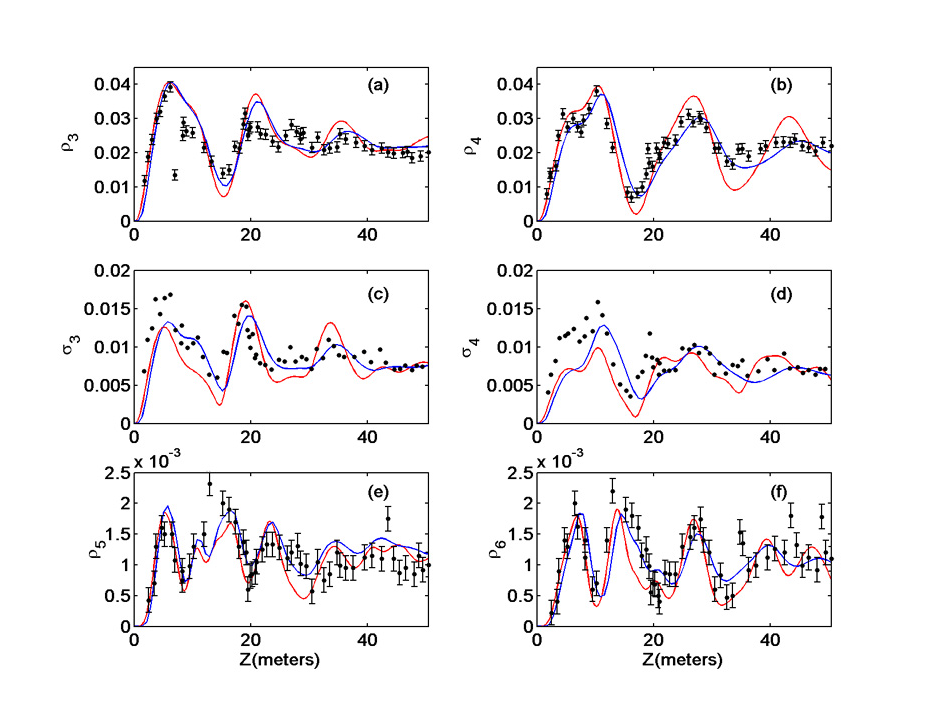
\includegraphics[width=6in]{nlsez55phaseornot.eps}
\end{center}
\renewcommand{\baselinestretch}{1}
\small\normalsize
\begin{quote}
\caption[Figure with caption indented]{This figure caption is indented and single-spaced.  Comparison between the experimental measurements \cite{hart1} (black), the random initial condition NLSE model excluding phase noise (dashed curves) and the stochastic phase noise NLSE model (solid curves) showing the first- and second-order sideband evolution as a function of fiber length for P$_{0} = 5.5$\,W, $\Omega = 366$\,GHz, $\Delta\nu = 0.5$\,GHz, $\gamma = 0.019$\,W$^{-1}$m$^{-1}$, and $\beta^{(2)} = 55$\,ps$^2$/km: dynamical evolution of the: (a) power in the first-order blue-shifted sideband, (b) power in the first-order red-shifted sideband, (c) fluctuations in the first-order blue-shifted sideband, (d) fluctuations in the first-order red-shifted sideband, (e) power in the second-order blue-shifted sideband, (f) power in the second-order red-shifted sideband. \label{fig:fig27}}
\end{quote}
\end{figure} 
\renewcommand{\baselinestretch}{2}
\small\normalsize

The first figure is Fig.\ref{fig:fig27}.   Please note that the figure label should be placed inside the figure caption.  
\newpage

The next figure is placed landscape.  It is Fig.~\ref{fig:mpc}.

\begin{landscape}
\renewcommand{\baselinestretch}{1}
\small\normalsize
\begin{quote}
\begin{figure}
\begin{center}
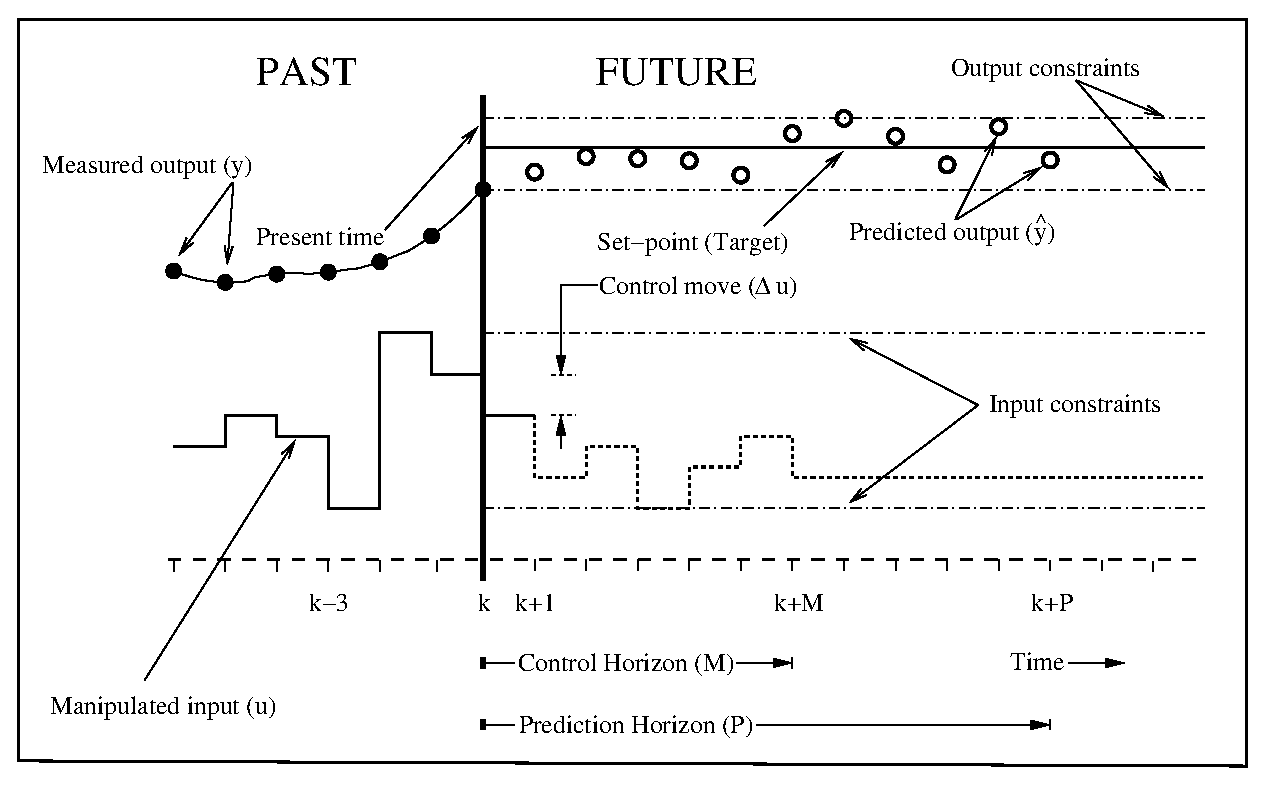
\includegraphics[width=8.2in]{mpc.eps}
\end{center}
\caption{Schematic illustrating receding horizon control.
\label{fig:mpc} }
\end{figure}
\end{quote}
\renewcommand{\baselinestretch}{2}
\small\normalsize
\end{landscape}

This is a my second figure which was placed landscape.  Although I have used the same figure, I have renamed the label to fig:mpc-1.  The second figure now becomes Figure~\ref{fig:mpc-1}.
\begin{landscape}
\renewcommand{\baselinestretch}{1}
\small\normalsize
\begin{quote}
\begin{figure}
\begin{center}
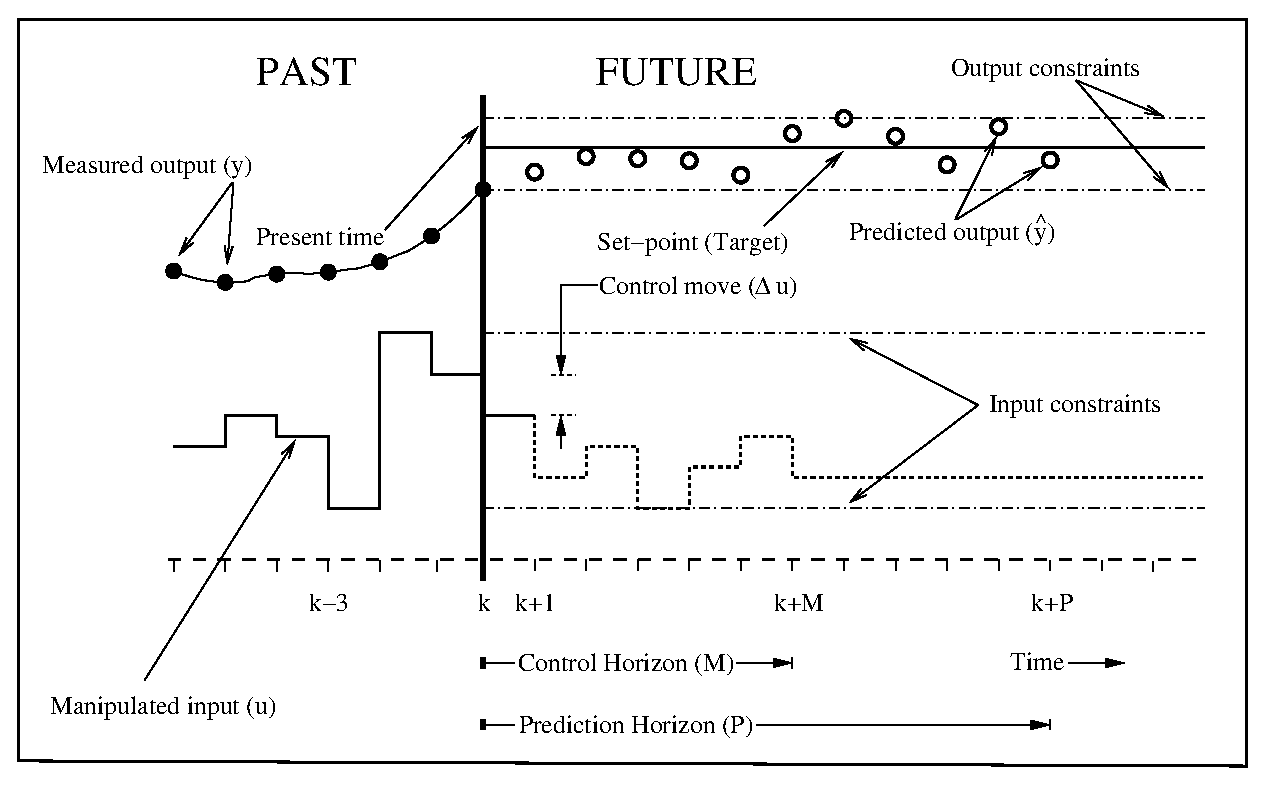
\includegraphics[width=8.2in]{mpc.eps}
\end{center}
\caption[Figure placed landscape on page]{Schematic illustrating receding horizon control. \label{fig:mpc-1}}
\end{figure}
\end{quote}
\renewcommand{\baselinestretch}{2}
\small\normalsize
\end{landscape}

\subsection{Numbering Figures}

If you wish your figures to be numbered 1-100 without any reference to the chapter (e.g., Figure 1.1, 2.1, etc.), change the first line of your mainthesis.tex file to read \begin{verbatim}"\documentclass[12pt]{thesis-2}".\end{verbatim}  

\subsubsection{This is a Subsubsection}

This is my first subsubsection in Chapter 1.


\section[Short Titles]{Short Titles in the Table of Contents, List of Figures, or List of Tables}

The Table of Contents, List of Figures, or List of Tables usually show the entire title of a section, subsection, etc. or table, or the entire caption of a figure.  If you put a short title in square brackets after \begin{verbatim} \section, \table, or \figure, \end{verbatim} the short title will show in your Table of Contents or lists.

\renewcommand{\baselinestretch}{1}
\small\normalsize

\begin{verbatim}
\section[Short Title]{Title of Section} 
\subsection[Short Title]{Title of Subsection} 
\end{verbatim}

or when using a caption in a figure or table
\begin{verbatim}
\caption[Short Caption]{Full text of the caption.}
\end{verbatim}

\renewcommand{\baselinestretch}{2}
\small\normalsize


\section{Figures on Text Page}

Normally figures in the thesis are placed on a page by themselves.  The following figure is placed on the page with text before and after the figure by adding [!!h] after \begin{verbatim} \begin{figure}[!!h] \end{verbatim}.  Please note that the figure label is placed within the caption.

\renewcommand{\baselinestretch}{1}
\large\normalsize

\begin{verbatim}
\begin{figure}[!!h]
 \begin{center}
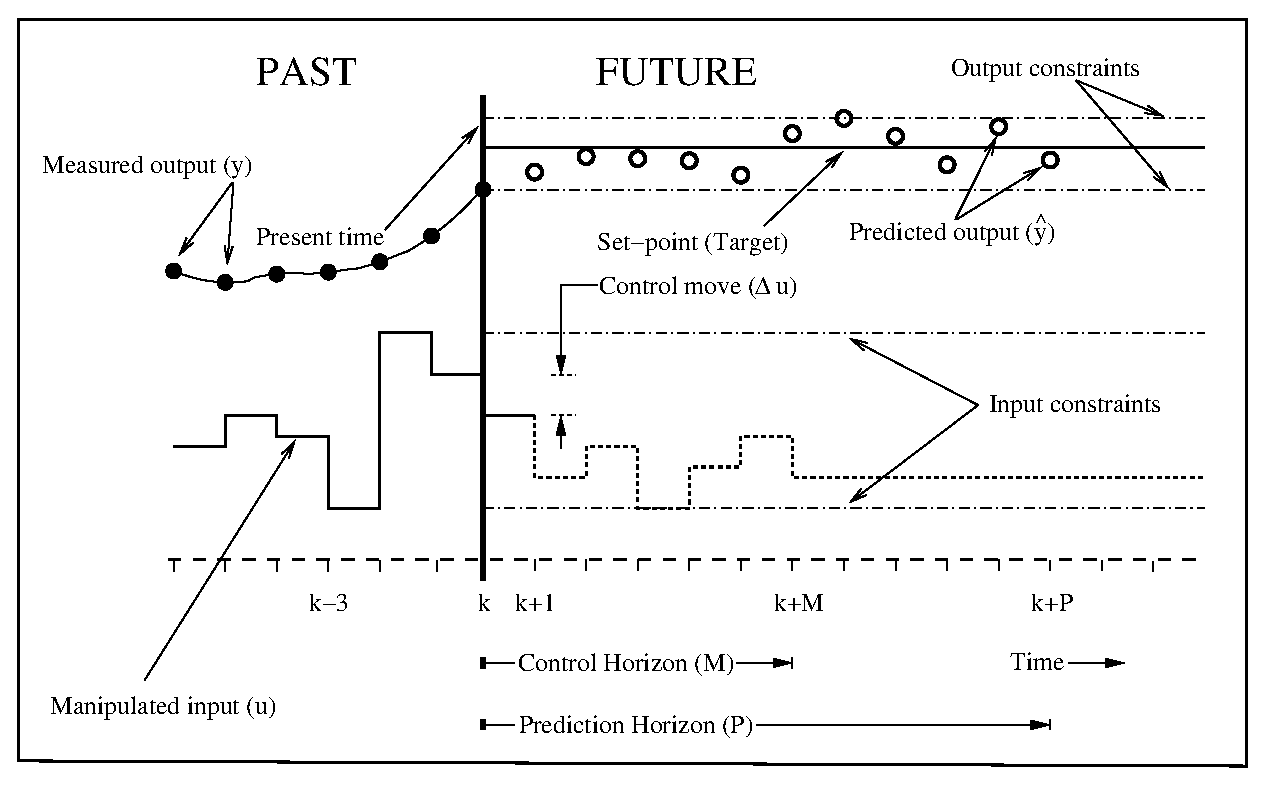
\includegraphics[width=5in]{mpc.eps}
\end{center}
\caption[Short title]{Schematic illustrating receding horizon control.
\label{fig:mpc-2}}
\end{figure}
\end{verbatim}

\begin{figure}[!!h]
 \begin{center}
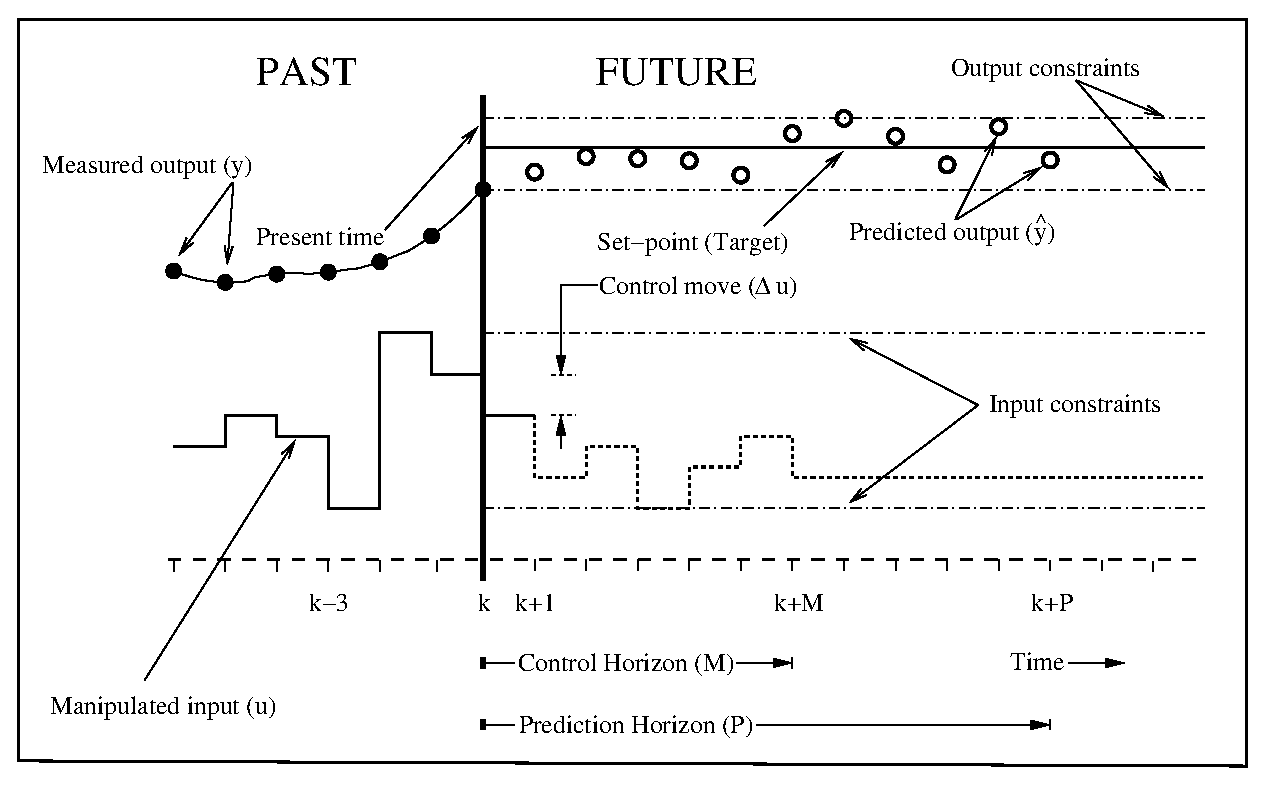
\includegraphics[width=5in]{mpc.eps}
\end{center}
\caption{Schematic illustrating receding horizon control. \label{fig:mpc-2}}
\end{figure}

\renewcommand{\baselinestretch}{2}
\large\normalsize

This does not necessarily mean that the text before and after the figure will be exactly what you want.  Remember Latex will place the figure where it will fit on the page the best.   The previous figure is Figs.~\ref{fig:mpc-2}. 

\section{Wrapping Text around Figure}


\renewcommand{\baselinestretch}{1}
\begin{wrapfigure}{r}{0.4\textwidth}
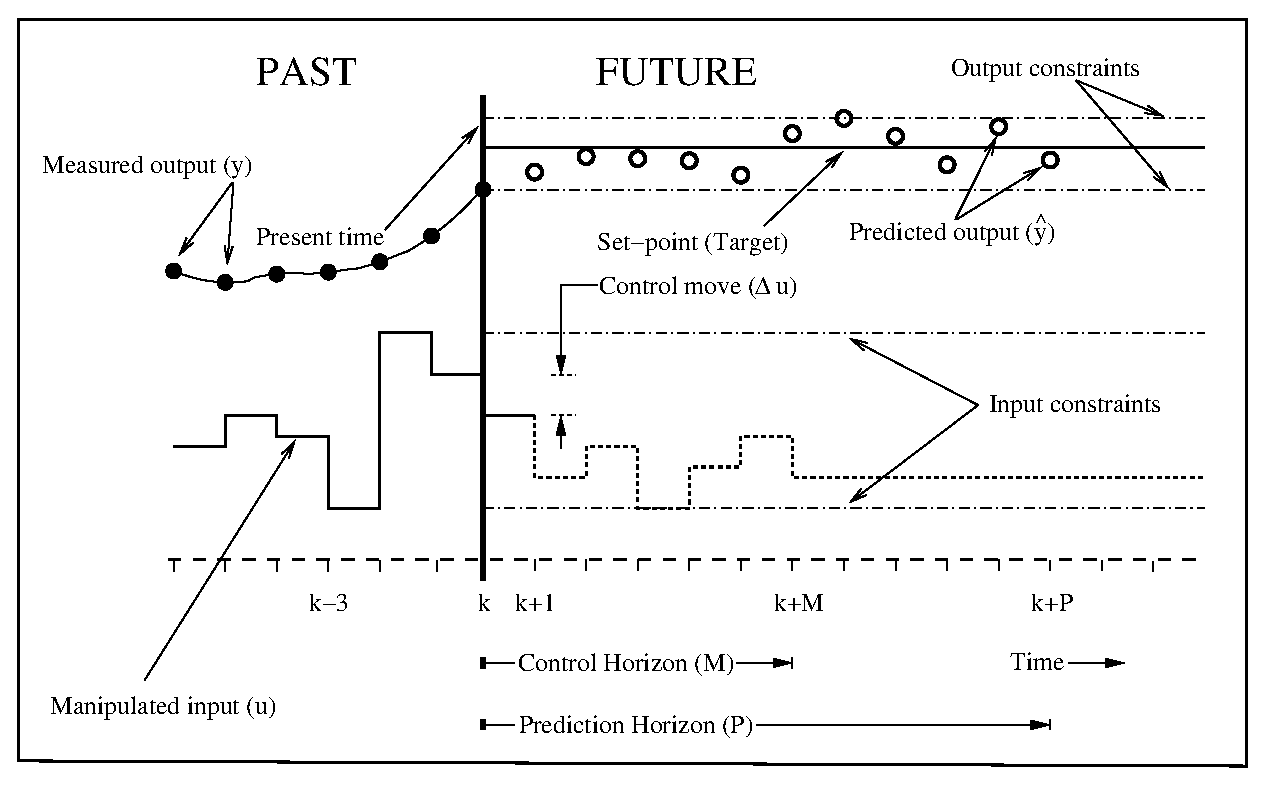
\includegraphics[width=0.4\textwidth]{mpc.eps}
\caption{ Text wrap around figure. \label{fig:test}}
\end{wrapfigure}

\renewcommand{\baselinestretch}{2}
\large\normalsize

By way of summary, at the end of the activity, I reminded the class of what we'd done:  by considering relatively nearby galaxies whose distance we had measured by some other means, we were able to establish a relationship locally between redshift and distance.  
By way of summary, at the end of the activity, I reminded the class of what we'd done:  by considering relatively nearby galaxies whose distance we had measured by some other means, we were able to establish a relationship locally between redshift and distance.  
By way of summary, at the end of the activity, I reminded the class of what we'd done:  by considering relatively nearby galaxies whose distance we had measured by some other means, we were able to establish a relationship locally between redshift and distance.  
By way of summary, at the end of the activity, I reminded the class of what we'd done:  by considering relatively nearby galaxies whose distance we had measured by some other means, we were able to establish a relationship locally between redshift and distance.  See Fig.~\ref{fig:test}.


\section{LaTeX -- A Typesetting Program}

A 13-page explanation of some of the features of LaTeX can be downloaded from http://www.jgsee.kmutt.ac.th/exell/General/LaTeX.html.


\section{Using Bibtex}

Using Bibtex with Latex documents is not difficult.  The bulk of the work is organizing your bibtex file, which is a data base compiled by you of the articles, books, etc. which you use in the bibliographies or reference sections of your publications.  

I have linked several files to this webpage, which will be helpful when you are using Bibtex.  These files can be downloaded from \newline
http://www.ireap.umd.edu/ireap/theses/bibtex.  Please read the file "BibtexInstructions.pdf".  The first two pages explain how to set up and run Bibtex; the remaining pages were taken from a published article and show how the references were cited in the .tex file.   The files BibtexInstructions.tex, Galactic.bib, Dottie.bib are the original .tex files used for BibtexInstructions.pdf.  The file BibtexSamples.tex contains examples of the information needed for the various publications you wish to reference (e.g., articles in refereed journals, books, unpublished articles, conference proceedings, etc.).

If you have questions concerning Bibtex, please contact me at 301-405-4955 or dbrosius at umd.edu.

\section{Using Natbib}

Another option of citing references in the bibliography is using Natbib instead of Bibtex.  You must still create a bibtex file, as noted above.  The command "backslash cite" cannot be used with natbib; instead "backslash citet" and "backslash citep" must be used.    "backslash citet" is used to show reference in the text (e.g., Eq.\ 8 in Reiser,1996 shows ...); "backslash citep" is used in the parenthetical (e.g., Eq.\ 8 (Reiser, 1996) shows ...).  

\begin{verbatim}
Add in preamble -- \usepackage[option]{natbib} 

Add at bottom of mainthesis.tex file --
\bibliography{name of your bibtex file}
\bibliographystyle{plainnat, abbrnat, or unsrtnat}
\end{verbatim}

Typesetting:   Latex, Bibtex, Latex, Latex

The reference sheet for natbib usage can be found at \newline "http://merkel.zoneo.net/Latex/natbib.php".

\section{APS Physical Review Style and Notation Guide}

The following style guide may be downloaded from The American Physical Society at http://forms.aps.org/author/styleguide.pdf:  Physical Review Style and Notation Guide, published by The American Physical Society, compiled and edited by Anne Waldron, Peggy Judd, and Valerie Miller, February 1993.  It may be old, but it is very useful.


%Chapter 2

\renewcommand{\thechapter}{2}

\chapter{Stochastic Four-Wave-Mixing}

\section{Overview}

The understanding of nonlinear processes in optical fibers is crucial towards 
extending the capabilities of modern optical communication systems based on 
wavelength division multiplexing (WDM), where each communication channel is 
represented by a unique wavelength. One of the nonlinear processes that 
limits the information carrying capacity of a WDM system is four-wave mixing 
(FWM), which causes cross-talk between neighboring channels. This places a 
lower limit on the wavelength separation between adjacent channels and an
upper limit on the input power in each channel. In this study, we describe
a process by which the evolution of FWM processes in an optical fiber can be 
used to estimate the inhomogeneities in the fiber core material, in particular 
the fluctuations in the linear refractive index of the fiber core.  

Experiments measuring the evolution of FWM processes along a length of fiber 
were carried out by Hart {\it et al.}\ \cite{hart1} and are described in detail in 
Sec.\ 2.2. In this experiment, two input pump waves at frequencies
$\omega_1$ and $\omega_2$, interacted with each other through the third-order 
nonlinearity of the fiber material to generate first-order sidebands at frequencies 
$\omega_3 = 2\omega_1 - \omega_2$ and $\omega_4 = 2\omega_2 - \omega_1$. 
These waves further interacted to produce second-order sidebands at 
$\omega_5 = 2\omega_3 - \omega_4$ and $\omega_6 = 2\omega_4 - \omega_3$. 
Higher-order sidebands were also generated. The normalized power in the 
sideband at frequency $\omega_m$ was represented by $\rho_m$. The 
evolution of the FWM processes was characterized by the evolution of 
$\rho_m$(z) as a function of fiber length z. 

In the present work, we make a quantitative comparison between these 
experimental results and our numerical results based on efficient algorithms 
\cite{Agrawal2} to solve the nonlinear Schr\"odinger equation (NLSE) that
governs the system. The numerical model, its underlying assumptions and
the results are described in Sec.\ 2.3. A realistic description of a 
standard single mode optical fiber must take into account the random phase 
perturbations a light wave undergoes while propagating through it, without 
disturbing the underlying conservative properties of the system. The NLSE 
needs to be suitably modified in order to incorporate the stochastic nature 
of the propagation. In order to preserve the conservative properties of the 
system, the stochastic terms in the NLSE must necessarily be multiplicative in 
nature as an additive term acts as a source or a sink. An algorithm that 
achieves this with linear, Gaussian, $\delta$-correlated noise is outlined in 
Sec.\ 2.3. This algorithm preserves the unconditional stability of the 
system. At the same time, care is taken to transform the stochastic NLSE from 
its original Ito representation \cite{ito} to the computationally feasible Stratanovich 
representation \cite{stratanovich} by compensating for the 
spurious linear drift that results from integrating such stochastic 
differential equations \cite{risken,werner2,drummond1,carter3}. The dominant 
sources of phase noise are discussed in Sec.\ 2.4. 

Conclusions on the relevance of the experiments of Hart {\it et al.}\ \cite{hart1} 
and the stochastic modeling presented here are summarized in Sec.\ 2.5.    

\section{Experimental and Computational Background}

In this work, we focus on tracing the evolution of the sidebands, generated 
through FWM, along a length of optical fiber. The FWM spectral evolution along
50\,m of fiber for two input pump power regimes (2.1\,W and 5.5\,W) was
investigated \cite{hart1}. In the 2.1\,W case, the sideband evolution followed a damped 
sinusoid along the length of the fiber. The experiments also found that the 
two first-order sidebands ($\rho_3$-blueshifted and $\rho_4$-redshifted from 
the two pumps) had different evolutions along the fiber (with different 
spatial wavelengths). For the 5.5\,W case, the evolution of both first- and 
second-order sidebands was measured. The damping in the first-order sidebands 
($\rho_3$ and $\rho_4$) occured faster than in the 2.1\,W case. Experiments 
probing the dependence of the sideband power on the input power (ranging from 
2\,W to 17\,W) were also performed at a fixed output length of 50\,m of the fiber.
At the same fiber length, the optical spectra for input powers ranging from 
2\,W to 17\,W were also recorded \cite{hart1}. The spectral envelopes were observed to fit 
well to a hyperbolic secant function and the fit parameters were recorded. 
Measurements with a high-resolution wavemeter showed that one of the two pumps 
consisted of two very closely spaced longitudinal modes 
($\Delta\nu\sim$ 0.5\,GHz) which were not resolved by the spectrometer used to 
record the FWM spectra. Inclusion of this multimode nature of the pump input 
in their model was found to alter the sideband dynamics dramatically and 
partly explained the asymmetry between the blue-shifted and red-shifted 
sidebands though it did not account for the damping in the sidebands. This 
was accounted for by adding weak phase fluctuations to the waves as they 
propagated along the fiber \cite{hart1}. The physical source of these phase fluctuations 
was not known at that time. However, the inclusion of the phase fluctuations 
into the model gave excellent qualitative and quantitative agreement with 
experiment. Their model involved integration of a system of coupled ODEs 
derived from the NLSE \cite{thompson1} by a process of truncation that 
retained only the leading frequency components (the pumps and the first- and 
second-order sidebands), a process justified by the fact that the input pump 
waves are well approximated by a combination of monochromatic waves. Their 
final numerical results are based on simulations using the truncated-ODE model
with Langevin noise terms representing phase fluctuations in the fiber. 
Another physical source of stochasticity in their experiment was the inherent 
power fluctuation in the lasers used as the input pumps. The level of 
fluctuations (5-20\%) was measured and incorporated appropriately into their 
model through stochastic initial conditions. This explained the evolution of 
the level of observed fluctuations in the sideband trajectories although it 
was found to be inadequate by itself, to account for the damping of the 
trajectories. They found that all three physical characteristics mentioned 
above, namely the multimode nature of the pump input, the stochastic phase 
fluctuations along the length of the fiber, and the stochastic initial power 
fluctuations were crucial to explaining the different features of the 
experimental measurements \cite{hart1}. 

\section{Stochastic NLSE Model}

In the present work, we have developed and implemented an unconditionally 
stable scheme for integrating the NLSE that successfully incorporates phase 
noise into the SSFM. Thus, we are now in a position to harness the high 
frequency / time resolution of the SSFM together with its efficient 
convergence properties. Due to these advances, we are now able to do 
simulations with much higher frequency resolution (60\,MHz as compared to 
300\,GHz in the ODE model). This high resolution, coupled with an appropriate 
convolution scheme, enables us to compare these simulated spectra with the 
composite spectra observed by the spectrometers which had a resolution of 
$\sim$ 60\,GHz. This was not possible with the truncated ODE model as the 
resolution of the simulated spectra in that case was $\sim$ 300\,GHz. For 
exactly the same levels of phase fluctuations, and initial condition 
fluctuations as used in Ref.\ \cite{hart1}, comparisons for the present NLSE 
model with the experimental sideband evolution functions $\rho_i(z)$ show 
excellent quantitative agreement. These results, along with the algorithms 
employed, are described in detail in this section. We have identified linear 
refractive index fluctuations along the fiber length to be a strong candidate 
for a physical source of the stochastic phase fluctuations. A comparison 
between the various possible sources is given in Sec.\ 2.4.

Under the assumption that the electric field of the light in the fiber has a 
slowly varying envelope $A(z,\tau)$, and that the fiber medium has an 
instantaneous nonlinear response, the system is well described by the 
nonlinear Schr\"{o}dinger equation (NLSE) with a linear multiplicative
stochastic term
%2.1
\begin{equation}
{\partial U \over \partial z} + {i\beta^{(2)} \over 2T_0^2} 
{\partial^2 U \over \partial\tau^2} + {\alpha U \over 2}
 + i\Gamma(z,\tau)U-i\gamma P_0 |U|^2 U = 0.
\end{equation}
$Z$ is distance along the length of the fiber, 
$U(z,\tau)=A(z,\tau)/\sqrt{P_0}$ is the complex electric field envelope 
$A(z,\tau)$ normalized to the absolute amplitude of the field $\sqrt{P_0}$, 
$P_0$ is the total power in the fiber, $\tau$ is time normalized to a 
convenient time scale $T_0(\sim 1\ ns)$ measured in a reference frame 
moving with the group velocity of the pulse [$\tau=(t-z/v_g)/T_0$]. The 
simulations are carried out for exactly the same physical parameters as the 
experiments and simulations reported by Hart {\it et al}.\ \cite{hart1}, i.e., 
$\beta^{(2)}=55\,(ps)^2/km$, is the group velocity dispersion of the fiber at 
the operating wavelength $\lambda_{0}\sim$ 632\,nm 
($k_0\sim 10^7\,m^{-1}$). A loss of $\sim$ 6\,dB/km gives $\alpha$ = 0.0014\,m$^{-1}$ as the 
loss in the fiber at this wavelength. The nonlinearity coefficient 
$\gamma=0.019\,W^{-1}m^{-1}$ is given by 
%2.2
\begin{equation}
\gamma = {\omega_{ave}n_2^I \over cA_{eff}},
\end{equation}
where $A_{eff}$ is the effective core area of the fiber,
$n_2^I$ is the Kerr coefficient for the intensity-dependent refractive index, and 
$\omega_{ave}$ is the average angular frequency of the wave envelope. 
$\Gamma(z,\tau)$ is a linear multiplicative phase noise field. In this study 
the noise field is assumed to be $\delta$-correlated in both space and time. 
The evolution of the FWM dynamics is found to be sensitive to the strength of 
this noise field. It can be physically interpreted as phase noise arising due 
to fluctuations in the linear refractive index of the fiber medium. A detailed 
discussion of its physical origin is given in Sec.\ 2.4.

The system was simulated using the Split-Step Fourier Method (SSFM) 
\cite{Agrawal2}. An algorithm for appropriately incorporating stochastic
phase fluctuations along the length of the fiber in the SSFM was developed
and is summarized below.

The NLSE is composed of linear and nonlinear terms, and can be written in operator form as
%2.3
\begin{eqnarray}
{\partial U \over \partial z} & = & (\hat{D}+\hat{S}+\hat{N})U \nonumber \\
\hat{D}& = & {-i\beta^{(2)} \over 2T_0^2}
{\partial^2 \over \partial\tau^2} - {\alpha \over 2} \nonumber \\
\hat{S} & = & i\Gamma(z,\tau) \nonumber \\
\hat{N} & = & i\gamma P_0|U|^2,
\end{eqnarray}
where $\hat{D}$, $\hat{S}$ and $\hat{N}$ are linear
(dispersive), nonlinear 
and stochastic operators, respectively. It has an exact solution for 
infinitesimal $\Delta z$ given by - 
%2.4
\begin{equation}
U(z + \Delta z,\tau) = exp[\Delta z(\hat{D} + \hat{S} + \hat{N})]U(z,\tau) ,
\end{equation}
which can be approximated by
%2.5
\begin{equation}
U(z + \Delta z,\tau) \approx exp[\Delta z \hat{D}]exp[\Delta z \hat{S}]exp[\Delta z \hat{N}]U(z,\tau) .
\end{equation}

The execution of $exp[\Delta z \hat{N}]$ is carried out in $\tau$-space:
%2.6
\begin{equation}
B_1(z,\tau)=exp[\Delta z \hat{N}]U(z,\tau) .
\end{equation}

The execution of $exp[\Delta z \hat{S}]$ and $exp[\Delta z \hat{D}]$ is 
carried out in $\omega$-space.

In particular, the stochastic phase fluctuations are introduced by modifying 
the phase $\phi_j$ of each frequency component $\omega_j$ of the complex 
field according to
%2.7
\begin{eqnarray}
B_2(z,\omega) & = & {\cal{F}}[B_1(z,\tau)] \nonumber \\
B_3(z,\omega_{j}) & = & exp[i \delta\phi(z,\omega_j)]B_2(z,\omega_j) ,
\end{eqnarray}
where $\cal{F}$ represents the Fourier transform operation.

This process only modifies the phase of each complex frequency component, 
leaving its absolute value unchanged. Thus the algorithm conserves the total 
power and the unconditional stability of the system.

The stochastic phase fluctuations $\delta\phi(z,\omega_j)$ are taken to be 
$\delta$-correlated in frequency as well as spatially along the fiber length. 
The Box-Muller algorithm \cite{boxmuller} was used to generate Gaussian random
deviates from computer-generated uniform random deviates $r_{1j}$ and $r_{2j}$
at each spatial step and for each frequency component $\omega_j$. The 
fluctuations are given by
%2.8
\begin{equation}
\delta\phi(z,\omega_{j}) = \sqrt{-2\sigma_{\phi}^2 \Delta z ln(r_{1j})}cos(2 \pi r_{2j}) .
\end{equation}

This is followed by the execution of $exp[\Delta z \hat{D}]$, which is also 
carried out in Fourier space, followed by the inverse transform
%2.9
\begin{equation}
U(z + \Delta z,\tau) = {\cal{F}}^{-1}[exp[\Delta z \hat{D}(i\omega)]B_{3}(z,\omega)] .
\end{equation}

$\hat{D}(i\omega)$ is obtained by replacing $(\partial / \partial \tau)$ 
by $i \omega$.

%Figure 2.1
\begin{figure}
\begin{center}
\includegraphics[0in,0in][3.25in,4.266in]{nlsetime.eps}
\end{center}
\renewcommand{\baselinestretch}{1}
\small\normalsize
\begin{quote}
\caption[Multimode pulse input to the NLSE]{Multimode pulse input to the NLSE: (a) input pulse in time
domain and (b) input spectrum.}
\label{fig2.1}
\end{quote}
\end{figure}
\renewcommand{\baselinestretch}{2}
\small\normalsize

The basic form of the initial complex wave envelope function is 
%2.11 
\begin {equation}
U(0,\tau) = exp \left( - {\tau^2 \over 2\tau_p^2} \right)
\left\{ 
\begin{array}{l}
exp\left( {i\Omega\tau \over 2} \right) + \\
exp\left( - {i\Omega\tau \over 2} \right)
\end{array}
\right\} ,
\end{equation}
where $\tau_p$ is the pulse width T$_p$ =5\,ns FWHM, normalized to the time scale 
T$_0$, $\Omega$=366\,GHz is the frequency detuning between the two laser 
sources normalized to a frequency scale $\Omega_0$ = 62.5\,MHz.  Figure 2.1(a) 
shows a plot of this pulse $|U(0,\tau)|^2$. The overall Gaussian envelope 
has an FWHM of 5\,ns, the closely spaced dark lines are due to the 366\,GHz 
($\sim$3\,ps) beating between the two input pump frequencies. The 2\,ns 
modulations on the pulse are due to the 0.5\,GHz mode-structure in the 
blue-shifted pump wave. Figure 2.1(b) shows the input spectrum of this pulse 
which consists of two highly monochromatic pump waves with a detuning of 
$\Omega$=366\,GHz. The spectrum of the blue-shifted pump, upon magnification, 
is seen to be composed of two very closely spaced peaks, with a separation of 
$\Delta\nu$=0.5\,GHz. Hart {\it et al}.\ \cite{hart1} did not use pulsed 
wave functions in their NLSE simulations as the size of the FFT required to do 
so made it computationally prohibitive at that time. The size of the FFT was 
chosen such that it would accommodate a time span of 16\,ns in order to go 
sufficiently far into the wings on the Gaussian pulse; and a frequency span of 
16\,THz in order to accommodate all the sidebands generated and prevent 
spurious effects due to the reflection boundary conditions implicit in the 
SSFM algorithm. These considerations dictated the size of the FFT to be 
$\geq$(16 THz)$\cdot$(16 ns) = 256000. The nearest power of 2 is 
2$^{18} = 262144$, which has been used throughout the present work. The 
incorporation of the pulsed nature of the light was found to be necessary in 
explaining the dynamics. From the perspective of the coupled amplitude 
equations used by Hart {\it et al}.\ \cite{hart1}, the present model is equivalent 
to a coupled-ODE model with $2^{18}$ coupled ODEs. 

%Figure 2.2
\begin{figure}
\begin{center}
\includegraphics[0in,0in][6in,4.572in]{modestruc21ornot.eps}
\end{center}
\renewcommand{\baselinestretch}{1}
\small\normalsize
\begin{quote}
\caption[Short caption for Figure 2.2.]
{Effects of inclusion of the multimode nature ($\Delta\nu = 0.5$\,GHz) of the blue-shifted input pump laser on the 1st order sideband evolution as a function of fiber length for P$_0 = 2.1$\,W. Dashed curves represent simulations without the multimode nature and solid curves represent simulations with the multimode nature. $\Omega = 366$\,GHz, $\gamma = 0.019$\,W$^{-1}$\,m$^{-1}$, and $\beta^{(2)} = 55$\,ps$^2$/km (a) power in the blue-shifted sideband, (b) power in the red-shifted sideband.}
\label{fig2.2}
\end{quote}
\end{figure}
\renewcommand{\baselinestretch}{1}
\small\normalsize

%Figure 2.3
\begin{figure}
\begin{center}
\includegraphics[0in,0in][6in,4.572in]{modestruc55ornot.eps}
\end{center}
\renewcommand{\baselinestretch}{1}
\small\normalsize
\begin{quote}
\caption[Effects of inclusion of the multimode nature]
{Effects of inclusion of the multimode nature ($\Delta\nu = 0.5$\,GHz) of the blue-shifted input pump laser on the 1st order sideband evolution as a function of fiber length for P$_0 = 5.5$\,W. Dashed curves represent simulations without the multimode nature and solid curves represent simulations with the multimode nature. $\Omega = 366$\,GHz, $\gamma = 0.019$\,W$^{-1}$\,m$^{-1}$, and $\beta^{(2)} = 55$\,ps$^2$/km (a) power in the first-order blue-shifted sideband, (b) power in the first-order red-shifted sideband, (c) power in the second-order blue-shifted sideband, (d) power in the second-order red-shifted sideband.}
\label{fig2.3}
\end{quote}
\end{figure}
\renewcommand{\baselinestretch}{1}
\small\normalsize

%Figure 2.4
\begin{figure}
\begin{center}
\includegraphics[0in,0in][6in,4.572in]{nlsez21cwpulse.eps}
\end{center}
\renewcommand{\baselinestretch}{1}
\small\normalsize
\begin{quote}
\caption[Effects of inclusion of the pulsed nature]
{Effects of inclusion of the pulsed nature (5\,ns FWHM) of the input pump laser light on the first-order sideband evolution as a function of fiber length for P$_0 = 2.1$\,W. Dashed curves represent cw simulations and solid curves represent pulsed simulations. $\Omega = 366$\,GHz, $\Delta\nu = 0.5$, $\gamma = 0.019$\,W$^{-1}$m$^{-1}$, and $\beta^{(2)} = 55$\,ps$^2$/,km (a) power in the blue-shifted sideband, (b) power in the red-shifted sideband.}
\label{fig2.4}
\end{quote}
\end{figure}
\renewcommand{\baselinestretch}{1}
\small\normalsize

%Figure 2.5
\begin{figure}
\begin{center}
\includegraphics[0in,0in][6in,4.572in]{nlsez55cwpulse.eps}
\end{center}
\renewcommand{\baselinestretch}{1}
\small\normalsize
\begin{quote}
\caption
[Other effects of inclusion of the pulsed nature]
{Effects of inclusion of the pulsed nature (5\,ns FWHM) of the input pump laser on the first- and second-order sideband evolution as a function of fiber length for P$_0 = 5.5$\,W. Dashed curves represent cw simulations and solid curves represent pulsed simulations. $\Omega = 366$\,GHz, $\Delta\nu = 0.5$, $\gamma = 0.019$\,W$^{-1}$m$^{-1}$, and $\beta^{(2)} = 55$\,ps$^2$/,km (a) power in the first-order blue-shifted sideband, (b) power in the first-order red-shifted sideband, (c) power in the second-order blue-shifted sideband, (d) power in the second-order red-shifted sideband.}
\label{fig2.5}
\end{quote}
\end{figure}
\renewcommand{\baselinestretch}{2}
\small\normalsize

Upon incorporation of the multimode nature of the blue input pump laser source 
and the stochastic fluctuations in the initial power in the lasers, the 
initial wave function takes the form
%2.11
\begin {equation}
U(0,\tau) = exp\left( - {\tau^2 \over 2\tau_p^2} \right)
\left\{
\begin{array}{l}
\sqrt{{1 + \delta\rho_1 \over 2}} 
\left[ \begin{array}{l}
exp \left( {i(\Omega+\Delta\nu)\tau \over 2} \right) + \\
exp \left( {i(\Omega-\Delta\nu)\tau \over 2} \right) 
\end{array} \right]\\
+ \sqrt{1 + \delta\rho_2} exp\left( - {i\Omega\tau \over 2} \right)
\end{array}
\right\}.
\end{equation}

\

\noindent $\Delta\nu = 0.5$\,GHz is the frequency separation between the two longitudinal 
modes in the blue-shifted pump. $\delta\rho_1$ and $\delta\rho_2$ are 
Gaussian random deviates (generated using the Box-Muller algorithm 
\cite{boxmuller}) that represent the initial power fluctuations in each of the 
pump laser sources. Their standard deviations were taken to be, 
$\sigma_{\rho_1} = 0.2$, $\sigma_{\rho_2} = 0.11$ for simulations from 0\,m to 
20\,m, $\sigma_{\rho_1} = 0.12$, $\sigma_{\rho_2} = 0.05$ for simulations from 
20\,m to 50\,m along the length of the fiber. This is exactly the same 
prescription used by Hart {\it et al}.\ \cite{hart1} in their simulations and is 
dictated by their experimental measurements of the fluctuations in the pump 
laser intensities.

At this point it is worth noting the effects of the inclusion of two attributes of 
the input laser light, namely, the multimode nature of the blue-shifted pump, and 
the pulsed nature of the input light (assumed to be cw in the simulations reported by 
Hart {\it et al}.\ \cite{hart1}). 

Figure 2.2 shows a comparison between simulations with (solid curves) and without (dashed curves) the multimode nature for an input pump power of 2.1 Watts. The simulations with the mode structure show the asymmetry between the blue- and red-shifted sideband evolution, in particular, the difference in spatial wavelength between the two, and a non-return to zero nature of the evolution, as observed in the experimental data (black dots with error bars). These features are absent in the simulations without mode-structure. $\rho_3$ and $\rho_4$ stands for the first order blue- and red-shifted sidebands respectively.  Figure 2.3 shows the corresponding comparison for the case of 5.5 Watts of input pump power.  Here, too, the simulations incorporating the multimode nature of the blue-shifted pump (solid curves) are seen to be an improvement over those not incorporating it (dashed curves). A feature of the experimental data (black dots with errorbars) is that for the $\rho_3$ sideband, the initial part of the evolution involves a peak followed by a shoulder, while for the $\rho_4$ sideband, the initial part of the evolution involves a shoulder followed by a peak. This feature, too, is seen to occur as a result of the inclusion of the multimode nature of the blue-shifted pump.  

The effect of inclusion of the pulsed nature of the input beam is seen in Fig.\ 2.4 (for the 2.1 Watt case) and Fig.\ 2.5 (for the 5.5 Watt case). The solid dashes represent simulations for a cw input beam and the solid curves represent those for a pulsed input beam. The incorporation of the pulsed nature clearly results in damping of the sideband trajectories which are seen to come closer to the experimental data \cite{hart1} (black dots with error bars). 

Use of the FFT algorithm makes evaluation relatively fast compared to other 
finite-difference schemes. The computational error is $O(\Delta z^2)$, thus 
the solution converges with decreasing spatial step-size $\Delta z$. 

The simulations were tested for the conservation of total power along the 
fiber length (by setting the loss $\alpha$ to zero) and for the conservation 
of asymmetry \cite{thompson1,hart1} given by 
%2.12
\begin{equation}
C(Z) = \sum_{i=1}^{\infty}(2i-1)[\rho_{2i-1}(Z)-\rho_{2i}(Z)] .
\end{equation}

A clearer picture of the evolution of the sidebands is obtained by plotting both the 
power in the sidebands and their standard deviations as a function of length along the fiber. Figures 2.6(a) and 2.6(b) show a comparison between simulation and experiment of the evolution 
of the first-order blue-shifted ($\rho_3$) and red-shifted ($\rho_4$) sidebands,  
respectively, for an input power of 2.1 W. The dashed curves represent NLSE simulations 
which include the stochastic nature of the input powers of the pump lasers but exclude 
the stochastic phase fluctuations added along the length of the fiber, an attribute 
which is included in the simulations represented by the solid curves. The black dots 
with error bars represent the experimental data. The measured sideband 
power, normalized to the total power in the fiber, is periodic in length but 
appears to be damping to a constant value. The measured data also show a clear 
difference between the spatial wavelengths of oscillation of the blue-shifted ($\rho_3$) and red-shifted ($\rho_4$) sidebands trajectories, respectively. Both these features are captured well by both the simulations. Figures 2.6(c) and 2.6(d) compare experimental and simulated 
measures of the evolution of the standard deviation in the sideband power 
along the fiber length. It is clearly observed that simulations with phase noise 
added to the light field along the length of the fiber (solid curves) are closer to the 
experimental data as compared to those that exclude this feature (dashed curves). This indicates
the instrumental nature of the phase fluctuations in explaining key features of the dynamics.

%Figure 2.6
\begin{figure}
\begin{center}
\includegraphics[0in,0in][6in,4.572in]{nlsez21phaseornot.eps}
\end{center}
\renewcommand{\baselinestretch}{1}
\small\normalsize
\begin{quote}
\caption
[Comparison between experiments measurements]
{Comparison between the experimental measurements \cite{hart1}(black), the random initial condition NLSE model excluding phase noise (dashed curves) and the stochastic phase noise NLSE model (solid curves) showing the first-order sideband evolution as a function of fiber length for P$_{0} = 2.1$\,W, $\Omega = 366$\,GHz, $\Delta\nu = 0.5$\,GHz,$\gamma = 0.019$\,W$^{-1}$m$^{-1}$, and $\beta^{(2)} = 55$ps$^2$/km: dynamical evolution of the: (a) power in the blue-shifted sideband, (b) power in the red-shifted sideband, (c) fluctuations in the blue-shifted sideband, (d) fluctuations in the red-shifted sideband.}
\label{fig2.6}
\end{quote}
\end{figure}
\renewcommand{\baselinestretch}{2}
\small\normalsize

The apparent damping of the periodic sideband trajectory is seen more 
dramatically in Figs.\ 2.7(a) and 2.7(b), which show the evolution of the 
first-order sideband power along the fiber for an input power of 5.5\,W. 
The two first-order sidebands evolve differently. They appear to 
damp to a constant value at a faster rate than for the case with an input pump 
power of 2.1\,W. Here again, NLSE simulations that incorporate phase noise along the length
of the fiber (solid curves) are much more successful in accurately capturing the dynamical features of the system than NLSE simulations that do not take this feature into account (dashed curves).  Figures 2.7(c) and 2.7(d) show a comparison between the simulated and measured standard deviations. Comparisons for the second-order blue-shifted ($\rho_5$) and red-shifted ($\rho_6$) sidebands, respectively, are shown in Figs.\ 2.7(e) and 2.7(f). 


%Figure 2.7
\begin{figure}
\begin{center}
\includegraphics[0in,0in][6in,4.572in]{nlsez55phaseornot.eps}
\end{center}
\renewcommand{\baselinestretch}{1}
\small\normalsize
\begin{quote}
\caption
[This figure caption is indented and single-spaced.]
{This figure caption is indented and single-spaced.  Comparison between the experimental measurements \cite{hart1} (black), the random initial condition NLSE model excluding phase noise (dashed curves) and the stochastic phase noise NLSE model (solid curves) showing the first- and second-order sideband evolution as a function of fiber length for P$_{0} = 5.5$\,W, $\Omega = 366$\,GHz, $\Delta\nu = 0.5$\,GHz, $\gamma = 0.019$\,W$^{-1}$m$^{-1}$, and $\beta^{(2)} = 55$\,ps$^2$/km: dynamical evolution of the: (a) power in the first-order blue-shifted sideband, (b) power in the first-order red-shifted sideband, (c) fluctuations in the first-order blue-shifted sideband, (d) fluctuations in the first-order red-shifted sideband, (e) power in the second-order blue-shifted sideband, (f) power in the second-order red-shifted sideband.}
\label{fig2.7}
\end{quote}
\end{figure} 
\renewcommand{\baselinestretch}{2}
\small\normalsize

The observed dynamical evolution of the sidebands is found to depend 
sensitively on the strength of the stochastic phase fluctuations. Yet, best 
agreement with the experimental results of Hart {\it et al}.\ \cite{hart1} is 
achieved with exactly the same noise strength $\sigma^2_\phi$ as used in 
their truncated ODE model, namely, $\sigma^2_\phi = 0.0067$\,m$^{-1}$. They 
report that including phase noise in their FWM calculations resulted in a 
spurious linear drift in the trajectories for the sideband power with length. 
To remove this artifact of the computations, they added a linear loss to their 
coupled ODEs. They set the loss coefficient $\alpha = 0.0046$\,m$^{-1}$ by 
finding the value that removed this increasing slope. We have observed exactly 
the same secular growth phenomenon for a wide range of the noise strength 
$\sigma^2_\phi$ and have arrived at an empirical prescription for $\alpha$ 
namely, $\alpha\sim\sigma^2_\phi$, where $\sigma^2_\phi$ is the 
variance of the added phase noise. This indicates the general nature of 
dynamics resulting from the addition of stochastic, $\delta$-correlated phase 
fluctuations to systems governed by nonlinear partial differential equations 
\cite{risken}. 

It is remarkable that the strength of the phase noise required is the same in 
both the 2.1\,W and the 5.5\,W cases. Further, it is worth noting that exactly 
the same noise strength was used by Hart {\it et al}.\ \cite{hart1}, the difference 
being that they introduced phase noise only in the pump frequencies, whereas 
we have introduced it in all the Fourier modes ($\sim2^{18}$). As a 
confirmation of this result, they also performed experiments and numerical 
simulations examining the sideband power dependence on the input power at a 
fixed length of 50.4\,m of the same fiber. We have repeated these simulations 
with the stochastic NLSE model and the results are shown in Figs.\ 2.8(a) 
(blue-shifted sideband) and 2.8(b) (red-shifted sideband). The experimental 
measurements of the sideband powers are represented by filled squares and the 
results of numerical simulations are represented by triangles (without phase 
noise) and by circles (with phase noise). The simulations are seen to follow 
the general trend seen in the experiments. As the pump power is increased, the 
triangles (without phase noise) start to disagree with experiment, whereas the 
circles (with phase noise) are much closer to experiment. The phase noise 
strength used in these simulations was exactly the same as that used in the 
simulations depicted in Figs.\ 2.6 and 2.7. The agreement between the phase noise 
simulations and the experimental data was (once again) highly sensitive to the 
noise strength. Since this experiment (unlike those shown in Figs.\ 2.2 - 2.7) 
is non-destructive, it can be used to deduce the strength of phase noise 
processes in a given optical fiber. It will be shown in Sec.\ 2.4 that a 
likely cause of the phase noise is fluctuation in the linear refractive index 
of the fiber. The noise strength deduced from the present computational study 
corresponds to a refractive index inhomogeneity of 
$\langle \Delta n^{2} \rangle \sim 10^{-16}$.   

%Figure 2.8
\begin{figure}
\hspace{1.25in}
\includegraphics[0in,0in][6in,4.572in]{nlsefinal.eps}
\renewcommand{\baselinestretch}{1}
\small\normalsize
\begin{quote}
\caption
[Comparison between the experiments measurements (filled squares]
{Comparison between the experimental measurements (filled squares), simulations without stochastic phase fluctuations (open triangles) and with stochastic phase fluctuations (open circles) of the first-order sideband power versus pump input power for L=50.39\,m, and $\Omega = 366$\,GHz: power in the (a) blue-shifted sideband and (b) red-shifted sideband.}
\label{fig2.8}
\end{quote}
\end{figure}

%Figure 2.9
\begin{figure}
\begin{center}
\includegraphics[0in,0in][6in,4.572in]{fig292.eps}
\end{center}
\renewcommand{\baselinestretch}{1}
\small\normalsize
\begin{quote}
\caption
[Evolution of the FWM spectrum]
{Evolution of the FWM spectrum along the fiber (a) P=2.1\,W, experiment, (b) P=5.5\,W, experiment, (c) P=2.1\,W, stochastic-NLSE model, (d) P=5.5\,W, stochastic-NLSE model.}
\label{fig2.9}
\end{quote}
\end{figure}
\renewcommand{\baselinestretch}{2}
\small\normalsize

Till now the comparisons between our simulations of the full NLSE and the 
truncated ODE model give basically the same results, although with much better 
agreement with experiment. However, the full NLSE can also provide a detailed 
comparison with the experimental spectra. This was not available from the 
truncated ODE model. The simulations reported in this work were carried out 
with a very high frequency and time resolution in order to incorporate the 
fact that the input light was not cw, but was composed of $\sim$ 5\,ns long 
pulses; and that the number of sidebands generated required the frequency 
spread of the FFT to be $\sim$ 16\,THz, while resolving a longitudinal 
mode-structure of $\Delta\nu$ $\sim 0.5$\,GHz. The spectral resolution used was 
$\sim$ 0.05\,GHz, whereas the spectrometer used to observe the spectra had a 
resolution 1000 times larger ($\sim$ 50\,GHz). To account for this difference, 
the simulated spectra were first convolved with a Gaussian of unit peak and 
62\,GHz FWHM, before they were compared with the observed spectra.  

Figures 2.9(a) and 2.9(b) show three-dimensional plots of the average experimental 
FWM output spectrum along the length of the fiber for input pump powers of 2.1\,W and 5.5\,W,
 respectively (courtesy Hart {\it et al}.\ \cite{hart1}). The vertical 
axis represents the intensity, normalized to the peak power in one of the 
input pumps, plotted on a logarithmic scale. The pump frequencies are centered 
on $+/-\Omega/2$ and the fiber length is increasing into the page. Figures 
9(c) and 9(d) show the corresponding comparisons based on simulations using 
the stochastic-NLSE model. The basic features of the spectral evolution are 
captured by the simulations. 

%Figure 1.20
\begin{figure}
\begin{center}
\includegraphics[0in,0in][6in,4.573in]{nlsespec.eps}
\end{center}
\renewcommand{\baselinestretch}{1}
\small\normalsize
\begin{quote}
\caption
[Experimental FWM output spectrum]
{Experimental FWM output spectrum (solid line), convolved spectra from simulations of the stochastic NLSE model (dashed line), and hyperbolic secant envelope fit (dotted line) for pump input powers P$_0$ of (a) 2.1\,W, (b) 5.5\,W, (c) 6.7\,W, (d) 8.3\,W, (e) 12.7\,W, (f) 17.4\,W, fiber length L$= 50.39$\,m, $\Omega = 366$\,GHz, $\Delta\nu = 0.5$\,GHz, $\gamma = 0.019$\,W$^{-1}$m$^{-1}$, and $\beta^{(2)} = 55$\,ps$^2$/km.}
\label{fig2.10}
\end{quote}
\end{figure}
\renewcommand{\baselinestretch}{2}
\small\normalsize

Hart {\it et al}.\ \cite{hart1} also documented the experimentally observed FWM 
output spectra for a fixed fiber length of 50.39 meters for 6 different input 
pump powers. They state the coefficients A and B of the hyperbolic secant 
envelopes that best fit the output spectra which are given by
%2.13
\begin{equation}
f(\omega) = Asech(B\omega) ,
\end{equation}
where A and B are the experimental fit parameters.

The hyperbolic secant parameters A and B, that best fit the simulated spectra 
are exactly the same as those that best fit the experimental spectra 
\cite{hart1} for all the 6 cases of input power considered. Figure 2.10 shows an 
overlap of the simulated spectra (dashed line), with the experimental spectra 
(solid line) and the experimental hyperbolic secant envelope (dotted line) for 
6 different pump powers, namely, (a) 2.1\,W, (b) 5.5\,W, (c) 6.7\,W, (d) 8.3\,W, (e) 
12.7\,W, (f) 17.4\,W. The hyperbolic secant parameters for each of these pump 
powers are (a) A=3.85 and B=0.36, (b) A=2.26 and B=0.27, (c) A=1.81, B=0.25, 
(d) A=1.56 and B=0.23, (e) A=0.98,B=0.20, and (f) A=0.81 and B=0.20. The exact 
shapes of the simulated spectra match very well with the experimental spectra 
for low input pump powers (2.1\,W and 5.5\,W), but tend to lack the "filled-in" 
character of the experimental spectra at higher powers (6.7\,W, 8.3\,W, 12.7\,W and 
17.4\,W).

\section{Discussion}

Hart {\it et al}.\ \cite{hart1} postulated that strong candidates for the possible 
physical sources of the phase fluctuations are stimulated Brillouin 
scattering, stimulated Raman scattering and fiber medium inhomogeneities. 
Brillouin scattering was eliminated as a source, since a backward propagating 
wave, which is a signature of Brillouin scattering in optical fibers, was not 
observed in the experiments. We have  modeled stimulated Raman scattering 
\cite{Agrawal8, headley} for our system and have found no evidence to
support the hypothesis that it could be a possible source of the stochastic phase 
fluctuations for fiber lengths up to 50 meters and pump power levels up to 5.5 Watts. 
A more detailed discussion of the Raman scattering simulations performed is given in Chap.\ 3.
Apart from these, quantum phase fluctuations are another well 
known, though extremely weak, source of phase noise in optical fibers 
\cite{Agrawal2,perlmutter1}.

Fiber medium inhomogeneities were identified as the major cause of the 
stochastic phase fluctuations. These inhomogeneities can manifest themselves 
through spatial and/or temporal fluctuations in the fiber parameters, namely, 
the linear refractive index $n_0$, the group velocity $v_g$, the group 
velocity dispersion $\beta^{(2)}$ and the nonlinearity 
$\gamma$ \cite{abdullaev}. Of these, the fluctuation in the linear refractive 
index was found to be the only source of phase fluctuation that had a 
significant effect on the dynamics. A relationship between the level of 
refractive index fluctuations and the  corresponding level of phase 
fluctuations has been arrived at. It is found that refractive index 
fluctuations as small as $\sigma_n^2 \sim 10^{-17}$\,m$^{-1}$ can cause the 
desired phase fluctuations. Possible sources of these refractive index 
fluctuations are discussed below.   

Consider the modified nonlinear Schr\"odinger equation (NLSE) which is
stated below, with the linear multiplicative noise term represented in terms of 
spatial and temporal fluctuations in the refractive index of the fiber.
%2.14
\begin{equation}
{\partial U \over \partial z} + {i\beta^{(2)} \over 2T_0^2} {\partial^2U \over \partial\tau^2} + {\alpha U \over 2} + ik_0 \delta n(z,\tau)U - i\gamma P_{0}|U|^2 U = 0 ,
\end{equation}
where $\delta n(z,\tau)$ is the spatial and temporal variation of the refractive 
index along the fiber. It can be caused by temperature and density 
fluctuations in the fiber \cite{glenn}. 

The thermodynamic estimate for $\Delta n$ is given by \cite{glenn}
%2.15
\begin{equation}
\langle \Delta n^{2} \rangle = {-kT\rho^2 \over V^2}  
\left( {\partial V \over \partial P} \right)_{T} 
\left( {\partial n \over \partial \rho} \right)_{T}^{2}
 + {kT^2 \over \rho VC_v} \left( {\partial n \over \partial T} \right)_{\rho}^2 .
\end{equation} 

This gives the mean-square index fluctuation in terms of the properties of 
the material. It can be rewritten as
%2.16
\begin{equation}
\langle \Delta n^{2} \rangle = {V_{\rho}+V_T \over V} = \langle \Delta n^{2} \rangle_{\rho}+\langle \Delta n^{2} \rangle_{T} .
\end{equation}

For a fiber of length z=1\,m and radius r=2.82\,$\mu$m 
(Volume V=2.5 $\times 10^{-12}$\,m$^3$), these have been calculated to be 
%2.17
\begin{eqnarray}
\langle \Delta n^2 \rangle_{\rho} \sim 10^{-21} & \equiv & \langle \Delta \rho^2 \rangle \sim 10^{-14} 
{kg^2 \over m^6}, \nonumber \\
\langle \Delta n^2 \rangle_T \sim 10^{-23} & \equiv & \langle \Delta T^2 \rangle \sim 10^{-12}~{^\circ}C^2 .
\end{eqnarray}

It should be noted that $\langle \Delta n^2 \rangle \propto (1/z) \Rightarrow \delta n \propto  (1 / \sqrt{z})$. The corresponding phase fluctuation that this would lead to in the NLSE is given by $\delta \phi=k_{0} \delta n z \propto \sqrt {z}$, which is equivalent to the prescription for incorporating phase fluctuations into the stochastic NLSE model described in Sec.\ 2.3, namely,  $\langle \Delta \phi^2 \rangle = 6.7 \times 10^{-3}z$. Hart {\it et al}.\ \cite{hart1} used the same prescription and the same noise strength in their truncated-ODE model. From this we can estimate the level of refractive index fluctuation that corresponds to the noise strength used in the simulations described in Sec.\ 2.3 
%2.18
\begin{eqnarray}
\langle \Delta n^2 \rangle = {6.7 \times 10^{-3} \over k_0^2} = 6.78 \times 10^{-17} \nonumber\\
\equiv \langle \Delta T^{2} \rangle \sim 10^{-6}~{^\circ}C^2 \equiv \Delta T \sim 10^{-3}~{^\circ}C 
\end{eqnarray}

The temperature coefficient of the refractive index of silica \cite{glenn}, 
$(\partial n / \partial T)_{\rho} \sim 10^{-5} ~{^\circ}C^{-1}$. Thus even small spatio-temporal temperature fluctuations of $\sim 10^{-3} ~{^\circ}C$ are enough to cause the inferred level of refractive index fluctuations.

The refractive index fluctuations could also be due to inhomogeneities in the 
density of the fiber material, frozen in at the time of manufacture of the 
fiber. The simulations were averaged over $\sim$ 600 iterations to get a good 
estimate of the power fluctuations in the sidebands. Initially, simulations 
were performed with a different phase noise distribution for each iteration. 
Later, a particular (arbitrary) phase noise distribution was selected and 
frozen for all the iterations.
This did not reduce the level of damping observed in the sideband trajectories 
provided that the strength of the phase noise was kept the same, thus 
indicating that density fluctuations induced during fiber manufacture could be 
a possible source. The phase noise was modeled as $\delta$-correlated in
both space and time. A more realistic approach would be to use correlated
noise. Numerical methods to incorporate linear multiplicative correlated noise 
into the NLSE have been developed by M.J. Werner {\it et al}.\ \cite{werner2}.

\section{Conclusions}

The role of stochasticity in the dynamical evolution of four-wave-mixing 
processes in an optical fiber has been investigated. This research consisted 
of theoretical and numerical computations. It focuses on tracing the evolution 
of the sidebands, generated through FWM, along a length of optical fiber. 
Detailed comparisons were made with the experimental results of 
Hart {\it et al}.\ \cite{hart1} and the agreement was excellent. The present work 
uses numerical techniques that have much higher resolution and better 
efficiency, and it presents a theoretical basis for the role of the 
stochasticity in the dynamics. The system is known to be governed by the 
nonlinear Schr\"odinger equation (NLSE) to a very good 
approximation \cite{Agrawal2}. 

A powerful technique that can be used for simulations of the stochastic NLSE 
is the Split-step Fourier Method (SSFM) \cite{Agrawal2}. An algorithm for the 
direct implementation of stochastic processes along the length of the fiber in 
the SSFM has been developed. The advantages of this approach with respect to 
the coupled-ODE approach are that we can carry out simulations with much 
higher frequency and time resolution without sacrificing computational 
efficiency.
 
The physical sources of these stochastic phase fluctuations are investigated 
quantitatively and are identified to be due to fluctuations in the linear 
refractive index of the fiber. Strong candidates for the causes of these 
refractive index fluctuations are temperature fluctuations in the fiber medium 
caused by the fluctuating temperature of the fiber environment, density 
fluctuations in the fiber medium frozen into the fiber during manufacture, and 
intrinsic thermodynamic fluctuations in the temperature and density of the 
fiber.  

The experiments performed by Hart {\it et al}.\ \cite{hart1} can be used to 
determine the level of these refractive index fluctuations in commercial 
fibers. Results described in Figs.\ 2 and 3 represent a destructive 
experiment that measures the sideband evolution with fiber length for a fixed 
input pump power, necessarily requiring the fiber to be cut repeatedly. The 
level of refractive index fluctuations can be used as a parameter in the 
simulations to best fit the experimental results. Alternatively, Fig.\ 4 
represents a non-destructive experiment that measures the sideband evolution 
with input pump power for a fixed fiber length. These experiments are found to 
be effective for estimating the refractive index fluctuations, as the dynamics 
is observed to be sensitively dependent on the strength of the phase 
fluctuations. 


%Chapter 3

\renewcommand{\thechapter}{3}

\chapter{Stochastic Four-Wave-Mixing}

\section{Overview}

The understanding of nonlinear processes in optical fibers is crucial towards 
extending the capabilities of modern optical communication systems based on 
wavelength division multiplexing (WDM), where each communication channel is 
represented by a unique wavelength. One of the nonlinear processes that 
limits the information carrying capacity of a WDM system is four-wave mixing 
(FWM), which causes cross-talk between neighboring channels. This places a 
lower limit on the wavelength separation between adjacent channels and an
upper limit on the input power in each channel. In this study, we describe
a process by which the evolution of FWM processes in an optical fiber can be 
used to estimate the inhomogeneities in the fiber core material, in particular 
the fluctuations in the linear refractive index of the fiber core.  

Experiments measuring the evolution of FWM processes along a length of fiber 
were carried out by Hart {\it et al.}\ \cite{hart1} and are described in detail in 
Sec.\ 2.2. In this experiment, two input pump waves at frequencies
$\omega_1$ and $\omega_2$, interacted with each other through the third-order 
nonlinearity of the fiber material to generate first-order sidebands at frequencies 
$\omega_3 = 2\omega_1 - \omega_2$ and $\omega_4 = 2\omega_2 - \omega_1$. 
These waves further interacted to produce second-order sidebands at 
$\omega_5 = 2\omega_3 - \omega_4$ and $\omega_6 = 2\omega_4 - \omega_3$. 
Higher-order sidebands were also generated. The normalized power in the 
sideband at frequency $\omega_m$ was represented by $\rho_m$. The 
evolution of the FWM processes was characterized by the evolution of 
$\rho_m$(z) as a function of fiber length z. 

In the present work, we make a quantitative comparison between these 
experimental results and our numerical results based on efficient algorithms 
\cite{Agrawal2} to solve the nonlinear Schr\"odinger equation (NLSE) that
governs the system. The numerical model, its underlying assumptions and
the results are described in Sec.\ 3.3. A realistic description of a 
standard single mode optical fiber must take into account the random phase 
perturbations a light wave undergoes while propagating through it, without 
disturbing the underlying conservative properties of the system. The NLSE 
needs to be suitably modified in order to incorporate the stochastic nature 
of the propagation. In order to preserve the conservative properties of the 
system, the stochastic terms in the NLSE must necessarily be multiplicative in 
nature as an additive term acts as a source or a sink. An algorithm that 
achieves this with linear, Gaussian, $\delta$-correlated noise is outlined in 
Sec.\ 3.3. This algorithm preserves the unconditional stability of the 
system. At the same time, care is taken to transform the stochastic NLSE from 
its original Ito representation \cite{ito} to the computationally feasible Stratanovich 
representation \cite{stratanovich} by compensating for the 
spurious linear drift that results from integrating such stochastic 
differential equations \cite{risken,werner2,drummond1,carter3}. The dominant 
sources of phase noise are discussed in Sec.\ 3.4. 

Conclusions on the relevance of the experiments of Hart {\it et al.}\ \cite{hart1} 
and the stochastic modeling presented here are summarized in Sec.\ 2.5.    

\section{Experimental and Computational Background}

In this work, we focus on tracing the evolution of the sidebands, generated 
through FWM, along a length of optical fiber. The FWM spectral evolution along
50\,m of fiber for two input pump power regimes (2.1\,W and 5.5\,W) was
investigated \cite{hart1}. In the 2.1\,W case, the sideband evolution followed a damped 
sinusoid along the length of the fiber. The experiments also found that the 
two first-order sidebands ($\rho_3$-blueshifted and $\rho_4$-redshifted from 
the two pumps) had different evolutions along the fiber (with different 
spatial wavelengths). For the 5.5\,W case, the evolution of both first- and 
second-order sidebands was measured. The damping in the first-order sidebands 
($\rho_3$ and $\rho_4$) occured faster than in the 2.1\,W case. Experiments 
probing the dependence of the sideband power on the input power (ranging from 
2\,W to 17\,W) were also performed at a fixed output length of 50\,m of the fiber.
At the same fiber length, the optical spectra for input powers ranging from 
2\,W to 17\,W were also recorded \cite{hart1}. The spectral envelopes were observed to fit 
well to a hyperbolic secant function and the fit parameters were recorded. 
Measurements with a high-resolution wavemeter showed that one of the two pumps 
consisted of two very closely spaced longitudinal modes 
($\Delta\nu\sim$ 0.5\,GHz) which were not resolved by the spectrometer used to 
record the FWM spectra. Inclusion of this multimode nature of the pump input 
in their model was found to alter the sideband dynamics dramatically and 
partly explained the asymmetry between the blue-shifted and red-shifted 
sidebands though it did not account for the damping in the sidebands. This 
was accounted for by adding weak phase fluctuations to the waves as they 
propagated along the fiber \cite{hart1}. The physical source of these phase fluctuations 
was not known at that time. However, the inclusion of the phase fluctuations 
into the model gave excellent qualitative and quantitative agreement with 
experiment. Their model involved integration of a system of coupled ODEs 
derived from the NLSE \cite{thompson1} by a process of truncation that 
retained only the leading frequency components (the pumps and the first- and 
second-order sidebands), a process justified by the fact that the input pump 
waves are well approximated by a combination of monochromatic waves. Their 
final numerical results are based on simulations using the truncated-ODE model
with Langevin noise terms representing phase fluctuations in the fiber. 
Another physical source of stochasticity in their experiment was the inherent 
power fluctuation in the lasers used as the input pumps. The level of 
fluctuations (5-20\%) was measured and incorporated appropriately into their 
model through stochastic initial conditions. This explained the evolution of 
the level of observed fluctuations in the sideband trajectories although it 
was found to be inadequate by itself, to account for the damping of the 
trajectories. They found that all three physical characteristics mentioned 
above, namely the multimode nature of the pump input, the stochastic phase 
fluctuations along the length of the fiber, and the stochastic initial power 
fluctuations were crucial to explaining the different features of the 
experimental measurements \cite{hart1}. 

\section{Stochastic NLSE Model}

In the present work, we have developed and implemented an unconditionally 
stable scheme for integrating the NLSE that successfully incorporates phase 
noise into the SSFM. Thus, we are now in a position to harness the high 
frequency / time resolution of the SSFM together with its efficient 
convergence properties. Due to these advances, we are now able to do 
simulations with much higher frequency resolution (60\,MHz as compared to 
300\,GHz in the ODE model). This high resolution, coupled with an appropriate 
convolution scheme, enables us to compare these simulated spectra with the 
composite spectra observed by the spectrometers which had a resolution of 
$\sim$ 60\,GHz. This was not possible with the truncated ODE model as the 
resolution of the simulated spectra in that case was $\sim$ 300\,GHz. For 
exactly the same levels of phase fluctuations, and initial condition 
fluctuations as used in Ref.\ \cite{hart1}, comparisons for the present NLSE 
model with the experimental sideband evolution functions $\rho_i(z)$ show 
excellent quantitative agreement. These results, along with the algorithms 
employed, are described in detail in this section. We have identified linear 
refractive index fluctuations along the fiber length to be a strong candidate 
for a physical source of the stochastic phase fluctuations. A comparison 
between the various possible sources is given in Sec.\ 3.4.

Under the assumption that the electric field of the light in the fiber has a 
slowly varying envelope $A(z,\tau)$, and that the fiber medium has an 
instantaneous nonlinear response, the system is well described by the 
nonlinear Schr\"{o}dinger equation (NLSE) with a linear multiplicative
stochastic term
%3.1
\begin{equation}
{\partial U \over \partial z} + {i\beta^{(2)} \over 2T_0^2} 
{\partial^2 U \over \partial\tau^2} + {\alpha U \over 2}
 + i\Gamma(z,\tau)U-i\gamma P_0 |U|^2 U = 0.
\end{equation}
$Z$ is distance along the length of the fiber, 
$U(z,\tau)=A(z,\tau)/\sqrt{P_0}$ is the complex electric field envelope 
$A(z,\tau)$ normalized to the absolute amplitude of the field $\sqrt{P_0}$, 
$P_0$ is the total power in the fiber, $\tau$ is time normalized to a 
convenient time scale $T_0(\sim 1\ ns)$ measured in a reference frame 
moving with the group velocity of the pulse [$\tau=(t-z/v_g)/T_0$]. The 
simulations are carried out for exactly the same physical parameters as the 
experiments and simulations reported by Hart {\it et al}.\ \cite{hart1}, i.e., 
$\beta^{(2)}=55\,(ps)^2/km$, is the group velocity dispersion of the fiber at 
the operating wavelength $\lambda_{0}\sim$ 632\,nm 
($k_0\sim 10^7\,m^{-1}$). A loss of $\sim$ 6\,dB/km gives $\alpha$ = 0.0014\,m$^{-1}$ as the 
loss in the fiber at this wavelength. The nonlinearity coefficient 
$\gamma=0.019\,W^{-1}m^{-1}$ is given by 
%3.2
\begin{equation}
\gamma = {\omega_{ave}n_2^I \over cA_{eff}},
\end{equation}
where $A_{eff}$ is the effective core area of the fiber,
$n_2^I$ is the Kerr coefficient for the intensity-dependent refractive index, and 
$\omega_{ave}$ is the average angular frequency of the wave envelope. 
$\Gamma(z,\tau)$ is a linear multiplicative phase noise field. In this study 
the noise field is assumed to be $\delta$-correlated in both space and time. 
The evolution of the FWM dynamics is found to be sensitive to the strength of 
this noise field. It can be physically interpreted as phase noise arising due 
to fluctuations in the linear refractive index of the fiber medium. A detailed 
discussion of its physical origin is given in Sec.\ 3.4.

The system was simulated using the Split-Step Fourier Method (SSFM) 
\cite{Agrawal2}. An algorithm for appropriately incorporating stochastic
phase fluctuations along the length of the fiber in the SSFM was developed
and is summarized below.

The NLSE is composed of linear and nonlinear terms, and can be written in operator form as
%3.3
\begin{eqnarray}
{\partial U \over \partial z} & = & (\hat{D}+\hat{S}+\hat{N})U \nonumber \\
\hat{D}& = & {-i\beta^{(2)} \over 2T_0^2}
{\partial^2 \over \partial\tau^2} - {\alpha \over 2} \nonumber \\
\hat{S} & = & i\Gamma(z,\tau) \nonumber \\
\hat{N} & = & i\gamma P_0|U|^2,
\end{eqnarray}
where $\hat{D}$, $\hat{S}$ and $\hat{N}$ are linear
(dispersive), nonlinear 
and stochastic operators, respectively. It has an exact solution for 
infinitesimal $\Delta z$ given by - 
%3.4
\begin{equation}
U(z + \Delta z,\tau) = exp[\Delta z(\hat{D} + \hat{S} + \hat{N})]U(z,\tau) ,
\end{equation}
which can be approximated by
%3.5
\begin{equation}
U(z + \Delta z,\tau) \approx exp[\Delta z \hat{D}]exp[\Delta z \hat{S}]exp[\Delta z \hat{N}]U(z,\tau) .
\end{equation}

The execution of $exp[\Delta z \hat{N}]$ is carried out in $\tau$-space:
%3.6
\begin{equation}
B_1(z,\tau)=exp[\Delta z \hat{N}]U(z,\tau) .
\end{equation}

The execution of $exp[\Delta z \hat{S}]$ and $exp[\Delta z \hat{D}]$ is 
carried out in $\omega$-space.

In particular, the stochastic phase fluctuations are introduced by modifying 
the phase $\phi_j$ of each frequency component $\omega_j$ of the complex 
field according to
%3.7
\begin{eqnarray}
B_2(z,\omega) & = & {\cal{F}}[B_1(z,\tau)] \nonumber \\
B_3(z,\omega_{j}) & = & exp[i \delta\phi(z,\omega_j)]B_2(z,\omega_j) ,
\end{eqnarray}
where $\cal{F}$ represents the Fourier transform operation.

This process only modifies the phase of each complex frequency component, 
leaving its absolute value unchanged. Thus the algorithm conserves the total 
power and the unconditional stability of the system.

The stochastic phase fluctuations $\delta\phi(z,\omega_j)$ are taken to be 
$\delta$-correlated in frequency as well as spatially along the fiber length. 
The Box-Muller algorithm \cite{boxmuller} was used to generate Gaussian random
deviates from computer-generated uniform random deviates $r_{1j}$ and $r_{2j}$
at each spatial step and for each frequency component $\omega_j$. The 
fluctuations are given by
%3.8
\begin{equation}
\delta\phi(z,\omega_{j}) = \sqrt{-2\sigma_{\phi}^2 \Delta z ln(r_{1j})}cos(2 \pi r_{2j}) .
\end{equation}

This is followed by the execution of $exp[\Delta z \hat{D}]$, which is also 
carried out in Fourier space, followed by the inverse transform
%3.9
\begin{equation}
U(z + \Delta z,\tau) = {\cal{F}}^{-1}[exp[\Delta z \hat{D}(i\omega)]B_{3}(z,\omega)] .
\end{equation}

$\hat{D}(i\omega)$ is obtained by replacing $(\partial / \partial \tau)$ 
by $i \omega$.

%Figure 3.1
\renewcommand{\baselinestretch}{1}
\small\normalsize
\begin{quote}
\begin{figure}
\begin{center}
\includegraphics[0in,0in][3.25in,4.266in]{nlsetime.eps}
\end{center}
\caption[Multimode pulse input to the NLSE]
{Multimode pulse input to the NLSE: (a) input pulse in time
domain and (b) input spectrum.}
\label{fig3.1}
\end{figure}
\end{quote}
\renewcommand{\baselinestretch}{2}
\small\normalsize

The basic form of the initial complex wave envelope function is 
%3.10 
\begin {equation}
U(0,\tau) = exp \left( - {\tau^2 \over 2\tau_p^2} \right)
\left\{ 
\begin{array}{l}
exp\left( {i\Omega\tau \over 2} \right) + \\
exp\left( - {i\Omega\tau \over 2} \right)
\end{array}
\right\} ,
\end{equation}
where $\tau_p$ is the pulse width T$_p$ =5\,ns FWHM, normalized to the time scale 
T$_0$, $\Omega$=366\,GHz is the frequency detuning between the two laser 
sources normalized to a frequency scale $\Omega_0$ = 62.5\,MHz.  Figure 3.1(a) 
shows a plot of this pulse $|U(0,\tau)|^2$. The overall Gaussian envelope 
has an FWHM of 5\,ns, the closely spaced dark lines are due to the 366\,GHz 
($\sim$3\,ps) beating between the two input pump frequencies. The 2\,ns 
modulations on the pulse are due to the 0.5\,GHz mode-structure in the 
blue-shifted pump wave. Figure 3.1(b) shows the input spectrum of this pulse 
which consists of two highly monochromatic pump waves with a detuning of 
$\Omega$=366\,GHz. The spectrum of the blue-shifted pump, upon magnification, 
is seen to be composed of two very closely spaced peaks, with a separation of 
$\Delta\nu$=0.5\,GHz. Hart {\it et al}.\ \cite{hart1} did not use pulsed 
wave functions in their NLSE simulations as the size of the FFT required to do 
so made it computationally prohibitive at that time. The size of the FFT was 
chosen such that it would accommodate a time span of 16\,ns in order to go 
sufficiently far into the wings on the Gaussian pulse; and a frequency span of 
16\,THz in order to accommodate all the sidebands generated and prevent 
spurious effects due to the reflection boundary conditions implicit in the 
SSFM algorithm. These considerations dictated the size of the FFT to be 
$\geq$(16 THz)$\cdot$(16 ns) = 256000. The nearest power of 2 is 
2$^{18} = 262144$, which has been used throughout the present work. The 
incorporation of the pulsed nature of the light was found to be necessary in 
explaining the dynamics. From the perspective of the coupled amplitude 
equations used by Hart {\it et al}.\ \cite{hart1}, the present model is equivalent 
to a coupled-ODE model with $2^{18}$ coupled ODEs. 

%Figure 3.2
\begin{figure}
\begin{center}
\includegraphics[0in,0in][6in,4.572in]{modestruc21ornot.eps}
\end{center}
\renewcommand{\baselinestretch}{1}
\small\normalsize
\begin{quote}
\caption[Short caption for Figure 3.2.]
{Effects of inclusion of the multimode nature ($\Delta\nu = 0.5$\,GHz) of the blue-shifted input pump laser on the 1st order sideband evolution as a function of fiber length for P$_0 = 2.1$\,W. Dashed curves represent simulations without the multimode nature and solid curves represent simulations with the multimode nature. $\Omega = 366$\,GHz, $\gamma = 0.019$\,W$^{-1}$\,m$^{-1}$, and $\beta^{(2)} = 55$\,ps$^2$/km (a) power in the blue-shifted sideband, (b) power in the red-shifted sideband.}
\label{fig3.2}
\end{quote}
\end{figure}

%Figure 3.3
\begin{figure}
\begin{center}
\includegraphics[0in,0in][6in,4.572in]{modestruc55ornot.eps}
\end{center}
\begin{quote}
\caption[Effects of inclusion of the multimode nature]
{Effects of inclusion of the multimode nature ($\Delta\nu = 0.5$\,GHz) of the blue-shifted input pump laser on the 1st order sideband evolution as a function of fiber length for P$_0 = 5.5$\,W. Dashed curves represent simulations without the multimode nature and solid curves represent simulations with the multimode nature. $\Omega = 366$\,GHz, $\gamma = 0.019$\,W$^{-1}$\,m$^{-1}$, and $\beta^{(2)} = 55$\,ps$^2$/km (a) power in the first-order blue-shifted sideband, (b) power in the first-order red-shifted sideband, (c) power in the second-order blue-shifted sideband, (d) power in the second-order red-shifted sideband.}
\label{fig3.3}
\end{quote}
\end{figure}


%Figure 3.4
\begin{figure}
\begin{center}
\includegraphics[0in,0in][6in,4.572in]{nlsez21cwpulse.eps}
\end{center}
\begin{quote}
\caption[Effects of inclusion of the pulsed nature]
{Effects of inclusion of the pulsed nature (5\,ns FWHM) of the input pump laser light on the first-order sideband evolution as a function of fiber length for P$_0 = 2.1$\,W. Dashed curves represent cw simulations and solid curves represent pulsed simulations. $\Omega = 366$\,GHz, $\Delta\nu = 0.5$, $\gamma = 0.019$\,W$^{-1}$m$^{-1}$, and $\beta^{(2)} = 55$\,ps$^2$/,km (a) power in the blue-shifted sideband, (b) power in the red-shifted sideband.}
\label{fig3.4}
\end{quote}
\end{figure}


%Figure 3.5
\begin{figure}
\begin{center}
\includegraphics[0in,0in][6in,4.572in]{nlsez55cwpulse.eps}
\end{center}
\begin{quote}
\caption
[Other effects of inclusion of the pulsed nature]
{Effects of inclusion of the pulsed nature (5\,ns FWHM) of the input pump laser on the first- and second-order sideband evolution as a function of fiber length for P$_0 = 5.5$\,W. Dashed curves represent cw simulations and solid curves represent pulsed simulations. $\Omega = 366$\,GHz, $\Delta\nu = 0.5$, $\gamma = 0.019$\,W$^{-1}$m$^{-1}$, and $\beta^{(2)} = 55$\,ps$^2$/,km (a) power in the first-order blue-shifted sideband, (b) power in the first-order red-shifted sideband, (c) power in the second-order blue-shifted sideband, (d) power in the second-order red-shifted sideband.}
\label{fig3.5}
\end{quote}
\end{figure}
\renewcommand{\baselinestretch}{2}
\small\normalsize

Upon incorporation of the multimode nature of the blue input pump laser source 
and the stochastic fluctuations in the initial power in the lasers, the 
initial wave function takes the form
%3.11
\begin {equation}
U(0,\tau) = exp\left( - {\tau^2 \over 2\tau_p^2} \right)
\left\{
\begin{array}{l}
\sqrt{{1 + \delta\rho_1 \over 2}} 
\left[ \begin{array}{l}
exp \left( {i(\Omega+\Delta\nu)\tau \over 2} \right) + \\
exp \left( {i(\Omega-\Delta\nu)\tau \over 2} \right) 
\end{array} \right]\\
+ \sqrt{1 + \delta\rho_2} exp\left( - {i\Omega\tau \over 2} \right)
\end{array}
\right\}.
\end{equation}

\

\noindent $\Delta\nu = 0.5$\,GHz is the frequency separation between the two longitudinal 
modes in the blue-shifted pump. $\delta\rho_1$ and $\delta\rho_2$ are 
Gaussian random deviates (generated using the Box-Muller algorithm 
\cite{boxmuller}) that represent the initial power fluctuations in each of the 
pump laser sources. Their standard deviations were taken to be, 
$\sigma_{\rho_1} = 0.2$, $\sigma_{\rho_2} = 0.11$ for simulations from 0\,m to 
20\,m, $\sigma_{\rho_1} = 0.12$, $\sigma_{\rho_2} = 0.05$ for simulations from 
20\,m to 50\,m along the length of the fiber. This is exactly the same 
prescription used by Hart {\it et al}.\ \cite{hart1} in their simulations and is 
dictated by their experimental measurements of the fluctuations in the pump 
laser intensities.

At this point it is worth noting the effects of the inclusion of two attributes of 
the input laser light, namely, the multimode nature of the blue-shifted pump, and 
the pulsed nature of the input light (assumed to be cw in the simulations reported by 
Hart {\it et al}.\ \cite{hart1}). 

Figure 3.2 shows a comparison between simulations with (solid curves) and without (dashed curves) the multimode nature for an input pump power of 2.1 Watts. The simulations with the mode structure show the asymmetry between the blue- and red-shifted sideband evolution, in particular, the difference in spatial wavelength between the two, and a non-return to zero nature of the evolution, as observed in the experimental data (black dots with error bars). These features are absent in the simulations without mode-structure. $\rho_3$ and $\rho_4$ stands for the first order blue- and red-shifted sidebands respectively.  Figure 3.3 shows the corresponding comparison for the case of 5.5 Watts of input pump power.  Here, too, the simulations incorporating the multimode nature of the blue-shifted pump (solid curves) are seen to be an improvement over those not incorporating it (dashed curves). A feature of the experimental data (black dots with errorbars) is that for the $\rho_3$ sideband, the initial part of the evolution involves a peak followed by a shoulder, while for the $\rho_4$ sideband, the initial part of the evolution involves a shoulder followed by a peak. This feature, too, is seen to occur as a result of the inclusion of the multimode nature of the blue-shifted pump.  

The effect of inclusion of the pulsed nature of the input beam is seen in Fig.\ 3.4 (for the 2.1 Watt case) and Fig.\ 3.5 (for the 5.5 Watt case). The solid dashes represent simulations for a cw input beam and the solid curves represent those for a pulsed input beam. The incorporation of the pulsed nature clearly results in damping of the sideband trajectories which are seen to come closer to the experimental data \cite{hart1} (black dots with error bars). 

Use of the FFT algorithm makes evaluation relatively fast compared to other 
finite-difference schemes. The computational error is $O(\Delta z^2)$, thus 
the solution converges with decreasing spatial step-size $\Delta z$. 

The simulations were tested for the conservation of total power along the 
fiber length (by setting the loss $\alpha$ to zero) and for the conservation 
of asymmetry \cite{thompson1,hart1} given by 
%3.12
\begin{equation}
C(Z) = \sum_{i=1}^{\infty}(2i-1)[\rho_{2i-1}(Z)-\rho_{2i}(Z)] .
\end{equation}

A clearer picture of the evolution of the sidebands is obtained by plotting both the 
power in the sidebands and their standard deviations as a function of length along the fiber. Figures 3.6(a) and 3.6(b) show a comparison between simulation and experiment of the evolution 
of the first-order blue-shifted ($\rho_3$) and red-shifted ($\rho_4$) sidebands,  
respectively, for an input power of 2.1 W. The dashed curves represent NLSE simulations 
which include the stochastic nature of the input powers of the pump lasers but exclude 
the stochastic phase fluctuations added along the length of the fiber, an attribute 
which is included in the simulations represented by the solid curves. The black dots 
with error bars represent the experimental data. The measured sideband 
power, normalized to the total power in the fiber, is periodic in length but 
appears to be damping to a constant value. The measured data also show a clear 
difference between the spatial wavelengths of oscillation of the blue-shifted ($\rho_3$) and red-shifted ($\rho_4$) sidebands trajectories, respectively. Both these features are captured well by both the simulations. Figures 3.6(c) and 2.6(d) compare experimental and simulated 
measures of the evolution of the standard deviation in the sideband power 
along the fiber length. It is clearly observed that simulations with phase noise 
added to the light field along the length of the fiber (solid curves) are closer to the 
experimental data as compared to those that exclude this feature (dashed curves). This indicates
the instrumental nature of the phase fluctuations in explaining key features of the dynamics.

%Figure 3.6
\begin{figure}
\begin{center}
\includegraphics[0in,0in][6in,4.572in]{nlsez21phaseornot.eps}
\end{center}
\renewcommand{\baselinestretch}{1}
\small\normalsize
\begin{quote}
\caption
[Comparison between experiments measurements]
{Comparison between the experimental measurements \cite{hart1}(black), the random initial condition NLSE model excluding phase noise (dashed curves) and the stochastic phase noise NLSE model (solid curves) showing the first-order sideband evolution as a function of fiber length for P$_{0} = 2.1$\,W, $\Omega = 366$\,GHz, $\Delta\nu = 0.5$\,GHz,$\gamma = 0.019$\,W$^{-1}$m$^{-1}$, and $\beta^{(2)} = 55$ps$^2$/km: dynamical evolution of the: (a) power in the blue-shifted sideband, (b) power in the red-shifted sideband, (c) fluctuations in the blue-shifted sideband, (d) fluctuations in the red-shifted sideband.}
\label{fig3.6}
\end{quote}
\end{figure}
\renewcommand{\baselinestretch}{2}
\small\normalsize

The apparent damping of the periodic sideband trajectory is seen more 
dramatically in Figs.\ 3.7(a) and 3.7(b), which show the evolution of the 
first-order sideband power along the fiber for an input power of 5.5\,W. 
The two first-order sidebands evolve differently. They appear to 
damp to a constant value at a faster rate than for the case with an input pump 
power of 2.1\,W. Here again, NLSE simulations that incorporate phase noise along the length
of the fiber (solid curves) are much more successful in accurately capturing the dynamical features of the system than NLSE simulations that do not take this feature into account (dashed curves).  Figures 3.7(c) and 3.7(d) show a comparison between the simulated and measured standard deviations. Comparisons for the second-order blue-shifted ($\rho_5$) and red-shifted ($\rho_6$) sidebands, respectively, are shown in Figs.\ 3.7(e) and 3.7(f). 


%Figure 3.7
\begin{figure}
\begin{center}
\includegraphics[0in,0in][6in,4.572in]{nlsez55phaseornot.eps}
\end{center}
\renewcommand{\baselinestretch}{1}
\small\normalsize
\begin{quote}
\caption
[This figure caption is indented and single-spaced]
{This figure caption is indented and single-spaced.  Comparison between the experimental measurements \cite{hart1} (black), the random initial condition NLSE model excluding phase noise (dashed curves) and the stochastic phase noise NLSE model (solid curves) showing the first- and second-order sideband evolution as a function of fiber length for P$_{0} = 5.5$\,W, $\Omega = 366$\,GHz, $\Delta\nu = 0.5$\,GHz, $\gamma = 0.019$\,W$^{-1}$m$^{-1}$, and $\beta^{(2)} = 55$\,ps$^2$/km: dynamical evolution of the: (a) power in the first-order blue-shifted sideband, (b) power in the first-order red-shifted sideband, (c) fluctuations in the first-order blue-shifted sideband, (d) fluctuations in the first-order red-shifted sideband, (e) power in the second-order blue-shifted sideband, (f) power in the second-order red-shifted sideband.}
\label{fig3.7}
\end{quote}
\end{figure} 
\renewcommand{\baselinestretch}{2}
\small\normalsize

The observed dynamical evolution of the sidebands is found to depend 
sensitively on the strength of the stochastic phase fluctuations. Yet, best 
agreement with the experimental results of Hart {\it et al}.\ \cite{hart1} is 
achieved with exactly the same noise strength $\sigma^2_\phi$ as used in 
their truncated ODE model, namely, $\sigma^2_\phi = 0.0067$\,m$^{-1}$. They 
report that including phase noise in their FWM calculations resulted in a 
spurious linear drift in the trajectories for the sideband power with length. 
To remove this artifact of the computations, they added a linear loss to their 
coupled ODEs. They set the loss coefficient $\alpha = 0.0046$\,m$^{-1}$ by 
finding the value that removed this increasing slope. We have observed exactly 
the same secular growth phenomenon for a wide range of the noise strength 
$\sigma^2_\phi$ and have arrived at an empirical prescription for $\alpha$ 
namely, $\alpha\sim\sigma^2_\phi$, where $\sigma^2_\phi$ is the 
variance of the added phase noise. This indicates the general nature of 
dynamics resulting from the addition of stochastic, $\delta$-correlated phase 
fluctuations to systems governed by nonlinear partial differential equations 
\cite{risken}. 

It is remarkable that the strength of the phase noise required is the same in 
both the 2.1\,W and the 5.5\,W cases. Further, it is worth noting that exactly 
the same noise strength was used by Hart {\it et al}.\ \cite{hart1}, the difference 
being that they introduced phase noise only in the pump frequencies, whereas 
we have introduced it in all the Fourier modes ($\sim2^{18}$). As a 
confirmation of this result, they also performed experiments and numerical 
simulations examining the sideband power dependence on the input power at a 
fixed length of 50.4\,m of the same fiber. We have repeated these simulations 
with the stochastic NLSE model and the results are shown in Figs.\ 3.8(a) 
(blue-shifted sideband) and 3.8(b) (red-shifted sideband). The experimental 
measurements of the sideband powers are represented by filled squares and the 
results of numerical simulations are represented by triangles (without phase 
noise) and by circles (with phase noise). The simulations are seen to follow 
the general trend seen in the experiments. As the pump power is increased, the 
triangles (without phase noise) start to disagree with experiment, whereas the 
circles (with phase noise) are much closer to experiment. The phase noise 
strength used in these simulations was exactly the same as that used in the 
simulations depicted in Figs.\ 3.6 and 3.7. The agreement between the phase noise 
simulations and the experimental data was (once again) highly sensitive to the 
noise strength. Since this experiment (unlike those shown in Figs.\ 3.2 - 3.7) 
is non-destructive, it can be used to deduce the strength of phase noise 
processes in a given optical fiber. It will be shown in Sec.\ 3.4 that a 
likely cause of the phase noise is fluctuation in the linear refractive index 
of the fiber. The noise strength deduced from the present computational study 
corresponds to a refractive index inhomogeneity of 
$\langle \Delta n^{2} \rangle \sim 10^{-16}$.   

%Figure 3.8
\begin{figure}
\hspace{1.25in}
\includegraphics[0in,0in][6in,4.572in]{nlsefinal.eps}
\begin{quote}
\caption
[Comparison between the experiments measurements (filled squares)]
{Comparison between the experimental measurements (filled squares), simulations without stochastic phase fluctuations (open triangles) and with stochastic phase fluctuations (open circles) of the first-order sideband power versus pump input power for L=50.39\,m, and $\Omega = 366$\,GHz: power in the (a) blue-shifted sideband and (b) red-shifted sideband.}
\label{fig3.8}
\end{quote}
\end{figure}

%Figure 3.9
\begin{figure}
\begin{center}
\includegraphics[0in,0in][6in,4.572in]{fig292.eps}
\end{center}
\begin{quote}
\caption
[Evolution of the FWM spectrum]
{Evolution of the FWM spectrum along the fiber (a) P=2.1\,W, experiment, (b) P=5.5\,W, experiment, (c) P=2.1\,W, stochastic-NLSE model, (d) P=5.5\,W, stochastic-NLSE model.}
\label{fig3.9}
\end{quote}
\end{figure}
\renewcommand{\baselinestretch}{2}
\small\normalsize

Till now the comparisons between our simulations of the full NLSE and the 
truncated ODE model give basically the same results, although with much better 
agreement with experiment. However, the full NLSE can also provide a detailed 
comparison with the experimental spectra. This was not available from the 
truncated ODE model. The simulations reported in this work were carried out 
with a very high frequency and time resolution in order to incorporate the 
fact that the input light was not cw, but was composed of $\sim$ 5\,ns long 
pulses; and that the number of sidebands generated required the frequency 
spread of the FFT to be $\sim$ 16\,THz, while resolving a longitudinal 
mode-structure of $\Delta\nu$ $\sim 0.5$\,GHz. The spectral resolution used was 
$\sim$ 0.05\,GHz, whereas the spectrometer used to observe the spectra had a 
resolution 1000 times larger ($\sim$ 50\,GHz). To account for this difference, 
the simulated spectra were first convolved with a Gaussian of unit peak and 
62\,GHz FWHM, before they were compared with the observed spectra.  

Figures 3.9(a) and 3.9(b) show three-dimensional plots of the average experimental 
FWM output spectrum along the length of the fiber for input pump powers of 2.1\,W and 5.5\,W,
 respectively (courtesy Hart {\it et al}.\ \cite{hart1}). The vertical 
axis represents the intensity, normalized to the peak power in one of the 
input pumps, plotted on a logarithmic scale. The pump frequencies are centered 
on $+/-\Omega/2$ and the fiber length is increasing into the page. Figures 
9(c) and 9(d) show the corresponding comparisons based on simulations using 
the stochastic-NLSE model. The basic features of the spectral evolution are 
captured by the simulations. 

%Figure 3.10
\begin{figure}
\begin{center}
\includegraphics[0in,0in][6in,4.573in]{nlsespec.eps}
\end{center}
\renewcommand{\baselinestretch}{1}
\small\normalsize
\begin{quote}
\caption
[Experimental FWM output spectrum]
{Experimental FWM output spectrum (solid line), convolved spectra from simulations of the stochastic NLSE model (dashed line), and hyperbolic secant envelope fit (dotted line) for pump input powers P$_0$ of (a) 2.1\,W, (b) 5.5\,W, (c) 6.7\,W, (d) 8.3\,W, (e) 12.7\,W, (f) 17.4\,W, fiber length L$= 50.39$\,m, $\Omega = 366$\,GHz, $\Delta\nu = 0.5$\,GHz, $\gamma = 0.019$\,W$^{-1}$m$^{-1}$, and $\beta^{(2)} = 55$\,ps$^2$/km.}
\label{fig3.10}
\end{quote}
\end{figure}
\renewcommand{\baselinestretch}{2}
\small\normalsize

Hart {\it et al}.\ \cite{hart1} also documented the experimentally observed FWM 
output spectra for a fixed fiber length of 50.39 meters for 6 different input 
pump powers. They state the coefficients A and B of the hyperbolic secant 
envelopes that best fit the output spectra which are given by
%2.13
\begin{equation}
f(\omega) = Asech(B\omega) ,
\end{equation}
where A and B are the experimental fit parameters.

The hyperbolic secant parameters A and B, that best fit the simulated spectra 
are exactly the same as those that best fit the experimental spectra 
\cite{hart1} for all the 6 cases of input power considered. Figure 2.10 shows an 
overlap of the simulated spectra (dashed line), with the experimental spectra 
(solid line) and the experimental hyperbolic secant envelope (dotted line) for 
6 different pump powers, namely, (a) 2.1\,W, (b) 5.5\,W, (c) 6.7\,W, (d) 8.3\,W, (e) 
12.7\,W, (f) 17.4\,W. The hyperbolic secant parameters for each of these pump 
powers are (a) A=3.85 and B=0.36, (b) A=2.26 and B=0.27, (c) A=1.81, B=0.25, 
(d) A=1.56 and B=0.23, (e) A=0.98,B=0.20, and (f) A=0.81 and B=0.20. The exact 
shapes of the simulated spectra match very well with the experimental spectra 
for low input pump powers (2.1\,W and 5.5\,W), but tend to lack the "filled-in" 
character of the experimental spectra at higher powers (6.7\,W, 8.3\,W, 12.7\,W and 
17.4\,W).

\section{Discussion}

Hart {\it et al}.\ \cite{hart1} postulated that strong candidates for the possible 
physical sources of the phase fluctuations are stimulated Brillouin 
scattering, stimulated Raman scattering and fiber medium inhomogeneities. 
Brillouin scattering was eliminated as a source, since a backward propagating 
wave, which is a signature of Brillouin scattering in optical fibers, was not 
observed in the experiments. We have  modeled stimulated Raman scattering 
\cite{Agrawal8, headley} for our system and have found no evidence to
support the hypothesis that it could be a possible source of the stochastic phase 
fluctuations for fiber lengths up to 50 meters and pump power levels up to 5.5 Watts. 
A more detailed discussion of the Raman scattering simulations performed is given in Chap.\ 3.
Apart from these, quantum phase fluctuations are another well 
known, though extremely weak, source of phase noise in optical fibers 
\cite{Agrawal2,perlmutter1}.

Fiber medium inhomogeneities were identified as the major cause of the 
stochastic phase fluctuations. These inhomogeneities can manifest themselves 
through spatial and/or temporal fluctuations in the fiber parameters, namely, 
the linear refractive index $n_0$, the group velocity $v_g$, the group 
velocity dispersion $\beta^{(2)}$ and the nonlinearity 
$\gamma$ \cite{abdullaev}. Of these, the fluctuation in the linear refractive 
index was found to be the only source of phase fluctuation that had a 
significant effect on the dynamics. A relationship between the level of 
refractive index fluctuations and the  corresponding level of phase 
fluctuations has been arrived at. It is found that refractive index 
fluctuations as small as $\sigma_n^2 \sim 10^{-17}$\,m$^{-1}$ can cause the 
desired phase fluctuations. Possible sources of these refractive index 
fluctuations are discussed below.   

Consider the modified nonlinear Schr\"odinger equation (NLSE) which is
stated below, with the linear multiplicative noise term represented in terms of 
spatial and temporal fluctuations in the refractive index of the fiber.
%3.14
\begin{equation}
{\partial U \over \partial z} + {i\beta^{(2)} \over 2T_0^2} {\partial^2U \over \partial\tau^2} + {\alpha U \over 2} + ik_0 \delta n(z,\tau)U - i\gamma P_{0}|U|^2 U = 0 ,
\end{equation}
where $\delta n(z,\tau)$ is the spatial and temporal variation of the refractive 
index along the fiber. It can be caused by temperature and density 
fluctuations in the fiber \cite{glenn}. 

The thermodynamic estimate for $\Delta n$ is given by \cite{glenn}
%3.15
\begin{equation}
\langle \Delta n^{2} \rangle = {-kT\rho^2 \over V^2}  
\left( {\partial V \over \partial P} \right)_{T} 
\left( {\partial n \over \partial \rho} \right)_{T}^{2}
 + {kT^2 \over \rho VC_v} \left( {\partial n \over \partial T} \right)_{\rho}^2 .
\end{equation} 

This gives the mean-square index fluctuation in terms of the properties of 
the material. It can be rewritten as
%3.16
\begin{equation}
\langle \Delta n^{2} \rangle = {V_{\rho}+V_T \over V} = \langle \Delta n^{2} \rangle_{\rho}+\langle \Delta n^{2} \rangle_{T} .
\end{equation}

For a fiber of length z=1\,m and radius r=2.82\,$\mu$m 
(Volume V=2.5 $\times 10^{-12}$\,m$^3$), these have been calculated to be 
%3.17
\begin{eqnarray}
\langle \Delta n^2 \rangle_{\rho} \sim 10^{-21} & \equiv & \langle \Delta \rho^2 \rangle \sim 10^{-14} 
{kg^2 \over m^6}, \nonumber \\
\langle \Delta n^2 \rangle_T \sim 10^{-23} & \equiv & \langle \Delta T^2 \rangle \sim 10^{-12}~{^\circ}C^2 .
\end{eqnarray}

It should be noted that $\langle \Delta n^2 \rangle \propto (1/z) \Rightarrow \delta n \propto  (1 / \sqrt{z})$. The corresponding phase fluctuation that this would lead to in the NLSE is given by $\delta \phi=k_{0} \delta n z \propto \sqrt {z}$, which is equivalent to the prescription for incorporating phase fluctuations into the stochastic NLSE model described in Sec.\ 2.3, namely,  $\langle \Delta \phi^2 \rangle = 6.7 \times 10^{-3}z$. Hart {\it et al}.\ \cite{hart1} used the same prescription and the same noise strength in their truncated-ODE model. From this we can estimate the level of refractive index fluctuation that corresponds to the noise strength used in the simulations described in Sec.\ 3.3 
%3.18
\begin{eqnarray}
\langle \Delta n^2 \rangle = {6.7 \times 10^{-3} \over k_0^2} = 6.78 \times 10^{-17} \nonumber\\
\equiv \langle \Delta T^{2} \rangle \sim 10^{-6}~{^\circ}C^2 \equiv \Delta T \sim 10^{-3}~{^\circ}C 
\end{eqnarray}

The temperature coefficient of the refractive index of silica \cite{glenn}, 
$(\partial n / \partial T)_{\rho} \sim 10^{-5} ~{^\circ}C^{-1}$. Thus even small spatio-temporal temperature fluctuations of $\sim 10^{-3} ~{^\circ}C$ are enough to cause the inferred level of refractive index fluctuations.

The refractive index fluctuations could also be due to inhomogeneities in the 
density of the fiber material, frozen in at the time of manufacture of the 
fiber. The simulations were averaged over $\sim$ 600 iterations to get a good 
estimate of the power fluctuations in the sidebands. Initially, simulations 
were performed with a different phase noise distribution for each iteration. 
Later, a particular (arbitrary) phase noise distribution was selected and 
frozen for all the iterations.
This did not reduce the level of damping observed in the sideband trajectories 
provided that the strength of the phase noise was kept the same, thus 
indicating that density fluctuations induced during fiber manufacture could be 
a possible source. The phase noise was modeled as $\delta$-correlated in
both space and time. A more realistic approach would be to use correlated
noise. Numerical methods to incorporate linear multiplicative correlated noise 
into the NLSE have been developed by M.J. Werner {\it et al}.\ \cite{werner2}.

\section{Conclusions}

The role of stochasticity in the dynamical evolution of four-wave-mixing 
processes in an optical fiber has been investigated. This research consisted 
of theoretical and numerical computations. It focuses on tracing the evolution 
of the sidebands, generated through FWM, along a length of optical fiber. 
Detailed comparisons were made with the experimental results of 
Hart {\it et al}.\ \cite{hart1} and the agreement was excellent. The present work 
uses numerical techniques that have much higher resolution and better 
efficiency, and it presents a theoretical basis for the role of the 
stochasticity in the dynamics. The system is known to be governed by the 
nonlinear Schr\"odinger equation (NLSE) to a very good 
approximation \cite{Agrawal2}. 

A powerful technique that can be used for simulations of the stochastic NLSE 
is the Split-step Fourier Method (SSFM) \cite{Agrawal2}. An algorithm for the 
direct implementation of stochastic processes along the length of the fiber in 
the SSFM has been developed. The advantages of this approach with respect to 
the coupled-ODE approach are that we can carry out simulations with much 
higher frequency and time resolution without sacrificing computational 
efficiency.
 
The physical sources of these stochastic phase fluctuations are investigated 
quantitatively and are identified to be due to fluctuations in the linear 
refractive index of the fiber. Strong candidates for the causes of these 
refractive index fluctuations are temperature fluctuations in the fiber medium 
caused by the fluctuating temperature of the fiber environment, density 
fluctuations in the fiber medium frozen into the fiber during manufacture, and 
intrinsic thermodynamic fluctuations in the temperature and density of the 
fiber.  

The experiments performed by Hart {\it et al}.\ \cite{hart1} can be used to 
determine the level of these refractive index fluctuations in commercial 
fibers. Results described in Figs.\ 2 and 3 represent a destructive 
experiment that measures the sideband evolution with fiber length for a fixed 
input pump power, necessarily requiring the fiber to be cut repeatedly. The 
level of refractive index fluctuations can be used as a parameter in the 
simulations to best fit the experimental results. Alternatively, Fig.\ 4 
represents a non-destructive experiment that measures the sideband evolution 
with input pump power for a fixed fiber length. These experiments are found to 
be effective for estimating the refractive index fluctuations, as the dynamics 
is observed to be sensitively dependent on the strength of the phase 
fluctuations. 


%%
%% This is file `supertabular.sty',
%% generated with the docstrip utility.
%%
%% The original source files were:
%%
%% supertabular.dtx  (with options: `package')
%% Copyright (C) 1989-2004 Johannes Braams. All rights reserved.
%% 
%% This file was generated from file(s) of the supertabular package.
%% -----------------------------------------------------------------
%% 
%% It may be distributed and/or modified under the
%% conditions of the LaTeX Project Public License, either version 1.3
%% of this license or (at your option) any later version.
%% The latest version of this license is in
%%   http://www.latex-project.org/lppl.txt
%% and version 1.3 or later is part of all distributions of LaTeX
%% version 2003/12/01 or later.
%% 
%% This work has the LPPL maintenance status "maintained".
%% 
%% The Current Maintainer of this work is Johannes Braams.
%% 
%% This file may only be distributed together with a copy of the
%% supertabular package. You may however distribute the supertabular package
%% without such generated files.
%% 
%% The list of all files belonging to the supertabular package is
%% given in the file `manifest.txt.
%% 
%% The list of derived (unpacked) files belonging to the distribution
%% and covered by LPPL is defined by the unpacking scripts (with
%% extension .ins) which are part of the distribution.
%% Sourcefile `supertabular.dtx'.
%%
%% Copyright (C) 1988 by Theo Jurriens
%% Copyright (C) 1990-2004 by Johannes Braams texniek at braams.cistron.nl
%%                            Kersengaarde 33
%%                            2723 BP Zoetermeer NL
%%                       all rights reserved.
%%
%%
\NeedsTeXFormat{LaTeX2e}
\ProvidesPackage{supertabular}
              [2004/02/20 v4.1e the supertabular environment]
\newcount\c@tracingst
\DeclareOption{errorshow}{\c@tracingst\z@}
\DeclareOption{pageshow}{\c@tracingst\tw@}
\DeclareOption{debugshow}{\c@tracingst5\relax}
\ProcessOptions
\newif\if@topcaption \@topcaptiontrue
\def\topcaption{\@topcaptiontrue\tablecaption}
\def\bottomcaption{\@topcaptionfalse\tablecaption}
\long\def\tablecaption{%
  \refstepcounter{table}\@dblarg{\@xtablecaption}}
\long\def\@xtablecaption[#1]#2{%
  \long\gdef\@process@tablecaption{\ST@caption{table}[#1]{#2}}}
\global\let\@process@tablecaption\relax
\newif\ifST@star
\newif\ifST@mp
\newdimen\ST@wd
\newskip\ST@rightskip
\newskip\ST@leftskip
\newskip\ST@parfillskip
\long\def\ST@caption#1[#2]#3{\par%
  \addcontentsline{\csname ext@#1\endcsname}{#1}%
                  {\protect\numberline{%
                      \csname the#1\endcsname}{\ignorespaces #2}}
  \begingroup
    \@parboxrestore
    \normalsize
    \if@topcaption \vskip -10\p@ \fi
    \@makecaption{\csname fnum@#1\endcsname}{\ignorespaces #3}\par
    \if@topcaption \vskip 10\p@ \fi
  \endgroup}
\newcommand\tablehead[1]{%
  \gdef\@tablehead{%
  \noalign{%
      \global\let\@savcr=\\
      \global\let\\=\org@tabularcr}%
    #1%
    \noalign{\global\let\\=\@savcr}}}
\tablehead{}
\newcommand\tablefirsthead[1]{\gdef\@table@first@head{#1}}
\newcommand\tabletail[1]{%
  \gdef\@tabletail{%
    \noalign{%
      \global\let\@savcr=\\
      \global\let\\=\org@tabularcr}%
    #1%
    \noalign{\global\let\\=\@savcr}}}
\tabletail{}
\newcommand\tablelasttail[1]{\gdef\@table@last@tail{#1}}
\newcommand\sttraceon{\c@tracingst5\relax}
\newcommand\sttraceoff{\c@tracingst\z@}
\newcommand\ST@trace[2]{%
  \ifnum\c@tracingst>#1\relax
    \GenericWarning
      {(supertabular)\@spaces\@spaces}
      {Package supertabular: #2}%
  \fi
  }
\newdimen\ST@pageleft
\newcommand*\shrinkheight[1]{%
  \noalign{\global\advance\ST@pageleft-#1\relax}}
\newcommand*\setSTheight[1]{%
  \noalign{\global\ST@pageleft=#1\relax}}
\newdimen\ST@headht
\newdimen\ST@tailht
\newdimen\ST@pagesofar
\newdimen\ST@pboxht
\newdimen\ST@lineht
\newdimen\ST@stretchht
\newdimen\ST@prevht
\newdimen\ST@toadd
\newdimen\ST@dimen
\newbox\ST@pbox
\def\ST@tabularcr{%
  {\ifnum0=`}\fi
  \@ifstar{\ST@xtabularcr}{\ST@xtabularcr}}
\def\ST@xtabularcr{%
  \@ifnextchar[%]
    {\ST@argtabularcr}%
    {\ifnum0=`{\fi}\cr\ST@cr}}
\def\ST@argtabularcr[#1]{%
  \ifnum0=`{\fi}%
  \ifdim #1>\z@
    \unskip\ST@xargarraycr{#1}
  \else
    \ST@yargarraycr{#1}%
  \fi}
\def\ST@xargarraycr#1{%
  \@tempdima #1\advance\@tempdima \dp \@arstrutbox
  \vrule \@height\z@ \@depth\@tempdima \@width\z@ \cr
  \noalign{\global\ST@toadd=#1}\ST@cr}
\def\ST@yargarraycr#1{%
  \cr\noalign{\vskip #1\global\ST@toadd=#1}\ST@cr}
\def\ST@startpbox#1{%
  \setbox\ST@pbox\vtop\bgroup\hsize#1\@arrayparboxrestore}
\def\ST@astartpbox#1{%
  \bgroup\hsize#1%
  \setbox\ST@pbox\vtop\bgroup\hsize#1\@arrayparboxrestore}
\def\ST@endpbox{%
  \@finalstrut\@arstrutbox\par\egroup
  \ST@dimen=\ht\ST@pbox
  \advance\ST@dimen by \dp\ST@pbox
  \ifnum\ST@pboxht<\ST@dimen
    \global\ST@pboxht=\ST@dimen
  \fi
  \ST@dimen=\z@
  \box\ST@pbox\hfil}
\def\ST@aendpbox{%
  \@finalstrut\@arstrutbox\par\egroup
  \ST@dimen=\ht\ST@pbox
  \advance\ST@dimen by \dp\ST@pbox
  \ifnum\ST@pboxht<\ST@dimen
    \global\ST@pboxht=\ST@dimen
  \fi
  \ST@dimen=\z@
  \unvbox\ST@pbox\egroup\hfil}
\def\estimate@lineht{%
  \ST@lineht=\arraystretch \baslineskp
  \global\advance\ST@lineht by 1\p@
  \ST@stretchht\ST@lineht\advance\ST@stretchht-\baslineskp
  \ifdim\ST@stretchht<\z@\ST@stretchht\z@\fi
  \ST@trace\tw@{Average line height: \the\ST@lineht}%
  \ST@trace\tw@{Stretched line height: \the\ST@stretchht}%
  }
\def\@calfirstpageht{%
  \ST@trace\tw@{Calculating height of tabular on first page}%
  \global\ST@pagesofar\pagetotal
  \global\ST@pageleft\@colroom
  \ST@trace\tw@{Height of text = \the\pagetotal; \MessageBreak
                Height of page = \the\ST@pageleft}%
  \if@twocolumn
    \ST@trace\tw@{two column mode}%
    \if@firstcolumn
     \ST@trace\tw@{First column}%
      \ifnum\ST@pagesofar > \ST@pageleft
        \global\ST@pageleft=2\ST@pageleft
        \ifnum\ST@pagesofar > \ST@pageleft
          \newpage\@calnextpageht
          \ST@trace\tw@{starting new page}%
        \else
          \ST@trace\tw@{Second column}%
          \global\advance\ST@pageleft -\ST@pagesofar
          \global\advance\ST@pageleft -\@colroom
        \fi
      \else
        \global\advance\ST@pageleft by -\ST@pagesofar
        \global\ST@pagesofar\z@
      \fi
    \else
      \ST@trace\tw@{Second column}
      \ifnum\ST@pagesofar > \ST@pageleft
        \ST@trace\tw@{starting new page}%
        \newpage\@calnextpageht
      \else
        \global\advance\ST@pageleft by -\ST@pagesofar
        \global\ST@pagesofar\z@
      \fi
    \fi
  \else
    \ST@trace\tw@{one column mode}%
    \ifnum\ST@pagesofar > \ST@pageleft
      \ST@trace\tw@{starting new page}%
      \newpage\@calnextpageht
    \else
      \global\advance\ST@pageleft by -\ST@pagesofar
      \global\ST@pagesofar\z@
    \fi
  \fi
  \ST@trace\tw@{Available height: \the\ST@pageleft}%
  \ifx\@@tablehead\@empty
    \ST@headht=\z@
  \else
    \setbox\@tempboxa=\vbox{\@arrayparboxrestore
      \ST@restore
      \expandafter\tabular\expandafter{\ST@tableformat}%
      \@@tablehead\endtabular}%
    \ST@headht=\ht\@tempboxa\advance\ST@headht\dp\@tempboxa
  \fi
  \ST@trace\tw@{Height of head: \the\ST@headht}%
  \ifx\@tabletail\@empty
    \ST@tailht=\z@
  \else
    \setbox\@tempboxa=\vbox{\@arrayparboxrestore
      \ST@restore
      \expandafter\tabular\expandafter{\ST@tableformat}
        \@tabletail\endtabular}
    \ST@tailht=\ht\@tempboxa\advance\ST@tailht\dp\@tempboxa
  \fi
  \advance\ST@tailht by \ST@lineht
  \ST@trace\tw@{Height of tail: \the\ST@tailht}%
  \ST@trace\tw@{Maximum height of tabular: \the\ST@pageleft}%
  \@tempdima\ST@headht
  \advance\@tempdima\ST@lineht
  \advance\@tempdima\ST@tailht
  \ST@trace\tw@{Minimum height of tabular: \the\@tempdima}%
  \ifnum\@tempdima>\ST@pageleft
    \ST@trace\tw@{starting new page}%
    \newpage\@calnextpageht
  \fi
}
\def\@calnextpageht{%
  \ST@trace\tw@{Calculating height of tabular on next page}%
  \global\ST@pageleft\@colroom
  \global\ST@pagesofar=\z@
  \ST@trace\tw@{Maximum height of tabular: \the\ST@pageleft}%
  }
\def\x@supertabular{%
  \let\org@tabular\tabular
  \let\tabular\inner@tabular
  \expandafter\let
    \csname org@tabular*\expandafter\endcsname
    \csname tabular*\endcsname
  \expandafter\let\csname tabular*\expandafter\endcsname
    \csname inner@tabular*\endcsname
  \if@topcaption \@process@tablecaption \fi
  \global\let\@oldcr=\\
  \def\baslineskp{\baselineskip}%
  \ifx\undefined\@classix
    \let\org@tabularcr\@tabularcr
    \let\@tabularcr\ST@tabularcr
    \let\org@startpbox=\@startpbox
    \let\org@endpbox=\@endpbox
    \let\@@startpbox=\ST@startpbox
    \let\@@endpbox=\ST@endpbox
  \else
    \let\org@tabularcr\@arraycr
    \let\@arraycr\ST@tabularcr
    \let\org@startpbox=\@startpbox
    \let\org@endpbox=\@endpbox
    \let\@startpbox=\ST@astartpbox
    \let\@endpbox=\ST@aendpbox
  \fi
  \ifx\@table@first@head\undefined
    \let\@@tablehead=\@tablehead
  \else
    \let\@@tablehead=\@table@first@head
  \fi
  \let\ST@skippage\ST@skipfirstpart
  \estimate@lineht
  \@calfirstpageht
  \noindent
  }
\def\supertabular{%
  \@ifnextchar[{\@supertabular}%]
               {\@supertabular[]}}
\def\@supertabular[#1]#2{%
  \def\ST@tableformat{#2}%
  \ST@trace\tw@{Starting a new supertabular}%
  \global\ST@starfalse
  \global\ST@mpfalse
  \x@supertabular
  \expandafter\org@tabular\expandafter{\ST@tableformat}%
  \@@tablehead}
\@namedef{supertabular*}#1{%
  \@ifnextchar[{\@nameuse{@supertabular*}{#1}}%
               {\@nameuse{@supertabular*}{#1}[]}%]
  }
\@namedef{@supertabular*}#1[#2]#3{%
  \ST@trace\tw@{Starting a new supertabular*}%
  \def\ST@tableformat{#3}%
  \ST@wd=#1\relax
  \global\ST@startrue
  \global\ST@mpfalse
  \x@supertabular
  \expandafter\csname org@tabular*\expandafter\endcsname
  \expandafter{\expandafter\ST@wd\expandafter}%
  \expandafter{\ST@tableformat}%
  \@@tablehead}%
\def\mpsupertabular{%
  \@ifnextchar[{\@mpsupertabular}%]
               {\@mpsupertabular[]}}
\def\@mpsupertabular[#1]#2{%
  \def\ST@tableformat{#2}%
  \ST@trace\tw@{Starting a new mpsupertabular}%
  \global\ST@starfalse
  \global\ST@mptrue
  \ST@rightskip \rightskip
  \ST@leftskip \leftskip
  \ST@parfillskip \parfillskip
  \x@supertabular
  \minipage{\columnwidth}%
  \parfillskip\ST@parfillskip
  \rightskip \ST@rightskip
  \leftskip \ST@leftskip
  \noindent\expandafter\org@tabular\expandafter{\ST@tableformat}%
  \@@tablehead}
\@namedef{mpsupertabular*}#1{%
  \@ifnextchar[{\@nameuse{@mpsupertabular*}{#1}}%
               {\@nameuse{@mpsupertabular*}{#1}[]}%]
  }
\@namedef{@mpsupertabular*}#1[#2]#3{%
  \ST@trace\tw@{Starting a new mpsupertabular*}%
  \def\ST@tableformat{#3}%
  \ST@wd=#1\relax
  \global\ST@startrue
  \global\ST@mptrue
  \ST@rightskip \rightskip
  \ST@leftskip \leftskip
  \ST@parfillskip \parfillskip
  \x@supertabular
  \minipage{\columnwidth}%
  \parfillskip\ST@parfillskip
  \rightskip \ST@rightskip
  \leftskip \ST@leftskip
  \noindent\expandafter\csname org@tabular*\expandafter\endcsname
  \expandafter{\expandafter\ST@wd\expandafter}%
  \expandafter{\ST@tableformat}%
  \@@tablehead}%
\def\endsupertabular{%
  \ifx\@table@last@tail\undefined
    \@tabletail
  \else
    \@table@last@tail
  \fi
  \csname endtabular\ifST@star*\fi\endcsname
  \ST@restore
  \if@topcaption
  \else
    \@process@tablecaption
    \@topcaptiontrue
  \fi
  \global\let\\\@oldcr
  \global\let\@process@tablecaption\relax
  \ST@trace\tw@{Ended a supertabular\ifST@star*\fi}%
  }
\expandafter\let\csname endsupertabular*\endcsname\endsupertabular
\def\endmpsupertabular{%
  \ifx\@table@last@tail\undefined
    \@tabletail
  \else
    \@table@last@tail
  \fi
  \csname endtabular\ifST@star*\fi\endcsname
  \endminipage
  \ST@restore
  \if@topcaption
  \else
    \@process@tablecaption
    \@topcaptiontrue
  \fi
  \global\let\\\@oldcr
  \global\let\@process@tablecaption\relax
  \ST@trace\tw@{Ended a mpsupertabular\ifST@star*\fi}%
  }
\expandafter\let\csname endmpsupertabular*\endcsname\endmpsupertabular
\def\ST@restore{%
  \ifx\undefined\@classix
    \let\@tabularcr\org@tabularcr
  \else
    \let\@arraycr\org@tabularcr
  \fi
  \let\@startpbox\org@startpbox
  \let\@endpbox\org@endpbox
  }
\def\inner@tabular{%
  \ST@restore
  \let\\\@oldcr
  \noindent
  \org@tabular}
\@namedef{inner@tabular*}{%
  \ST@restore
  \let\\\@oldcr
  \noindent
  \csname org@tabular*\endcsname}
\def\ST@cr{%
  \noalign{%
    \ifnum\ST@pboxht<\ST@lineht
      \global\advance\ST@pageleft -\ST@lineht
      \global\ST@prevht\ST@lineht
    \else
     \ST@trace\thr@@{Added par box with height \the\ST@pboxht}%
      \global\advance\ST@pageleft -\ST@pboxht
      \global\advance\ST@pageleft -0.1\ST@pboxht
      \global\advance\ST@pageleft -\ST@stretchht
      \global\ST@prevht\ST@pboxht
      \global\ST@pboxht\z@
    \fi
    \global\advance\ST@pageleft -\ST@toadd
    \global\ST@toadd=\z@
    \ST@trace\thr@@{Space left for tabular: \the\ST@pageleft}%
  }
  \noalign{\global\let\ST@next\@empty}%
  \ifnum\ST@pageleft<\z@
    \ST@skippage
  \else
    \noalign{\global\@tempdima\ST@tailht
      \global\advance\@tempdima\ST@prevht
    \ifST@mp
      \ifvoid\@mpfootins\else
        \global\advance\@tempdima\ht\@mpfootins
        \global\advance\@tempdima 3pt
      \fi
    \fi}
    \ifnum\ST@pageleft<\@tempdima
      \ST@newpage
    \fi
  \fi
  \ST@next}
\def\ST@skipfirstpart{%
  \noalign{%
    \ST@trace\tw@{Tabular too high, moving to next page}%
    \global\advance\ST@pageleft\pagetotal
    \global\ST@pagesofar\z@
    \newpage
    \global\let\ST@skippage\ST@newpage
    }}
\def\ST@newpage{%
  \noalign{\ST@trace\tw@{Starting new page, writing tail}}%
  \@tabletail
  \ifST@star
    \csname endtabular*\endcsname
  \else
    \endtabular
  \fi
  \ifST@mp
    \endminipage
  \fi
  \global\let\ST@skippage\ST@newpage
  \newpage\@calnextpageht
  \let\ST@next\@tablehead
  \ST@trace\tw@{writing head}%
  \ifST@mp
    \noindent\minipage{\columnwidth}%
    \parfillskip\ST@parfillskip
    \rightskip \ST@rightskip
    \leftskip \ST@leftskip
  \fi
  \noindent
  \ifST@star
    \expandafter\csname org@tabular*\expandafter\endcsname
    \expandafter{\expandafter\ST@wd\expandafter}%
    \expandafter{\ST@tableformat}%
  \else
    \expandafter\org@tabular\expandafter{\ST@tableformat}%
  \fi}
\endinput
%%
%% End of file `supertabular.sty'.

\titleformat{\chapter}
      {\normalfont\large}{Appendix \thechapter:}{1em}{}
%Appendix -- January 2015
\appendix
\renewcommand{\thechapter}{A}
\renewcommand{\chaptername}{Appendix}

\chapter{Previous Experiments}

The understanding of nonlinear processes in optical fibers is crucial towards 
extending the capabilities of modern optical communication systems based on 
wavelength division multiplexing (WDM), where each communication channel is 
represented by a unique wavelength. One of the nonlinear processes that 
limits the information carrying capacity of a WDM system is four-wave mixing 
(FWM), which causes cross-talk between neighboring channels. This places a 
lower limit on the wavelength separation between adjacent channels and an
upper limit on the input power in each channel. In this study, we describe
a process by which the evolution of FWM processes in an optical fiber can be 
used to estimate the inhomogeneities in the fiber core material, in particular 
the fluctuations in the linear refractive index of the fiber core.  

\section{Overview}

Experiments measuring the evolution of FWM processes along a length of fiber 
were carried out by Hart {\it et al.}\ \cite{hart1} and are described in detail in 
Sec.\ 2.2. In this experiment, two input pump waves at frequencies
$\omega_1$ and $\omega_2$, interacted with each other through the third-order 
nonlinearity of the fiber material to generate first-order sidebands at frequencies 
$\omega_3 = 2\omega_1 - \omega_2$ and $\omega_4 = 2\omega_2 - \omega_1$. 
These waves further interacted to produce second-order sidebands at 
$\omega_5 = 2\omega_3 - \omega_4$ and $\omega_6 = 2\omega_4 - \omega_3$. 
Higher-order sidebands were also generated. The normalized power in the 
sideband at frequency $\omega_m$ was represented by $\rho_m$. The 
evolution of the FWM processes was characterized by the evolution of 
$\rho_m$(z) as a function of fiber length z. 

In the present work, we make a quantitative comparison between these 
experimental results and our numerical results based on efficient algorithms 
\cite{Agrawal2} to solve the nonlinear Schr\"odinger equation (NLSE) that
governs the system. The numerical model, its underlying assumptions and
the results are described in Sec.\ 2.3. A realistic description of a 
standard single mode optical fiber must take into account the random phase 
perturbations a light wave undergoes while propagating through it, without 
disturbing the underlying conservative properties of the system. The NLSE 
needs to be suitably modified in order to incorporate the stochastic nature 
of the propagation. In order to preserve the conservative properties of the 
system, the stochastic terms in the NLSE must necessarily be multiplicative in 
nature as an additive term acts as a source or a sink. An algorithm that 
achieves this with linear, Gaussian, $\delta$-correlated noise is outlined in 
Sec.\ 2.3. This algorithm preserves the unconditional stability of the 
system. At the same time, care is taken to transform the stochastic NLSE from 
its original Ito representation \cite{ito} to the computationally feasible Stratanovich 
representation \cite{stratanovich} by compensating for the 
spurious linear drift that results from integrating such stochastic 
differential equations \cite{risken,werner2,drummond1,carter3}. The dominant 
sources of phase noise are discussed in Sec.\ 2.4. 

Conclusions on the relevance of the experiments of Hart {\it et al.}\ \cite{hart1} 
and the stochastic modeling presented here are summarized in Sec.\ 2.5.    

\section{Experimental and Computational Background}

In this work, we focus on tracing the evolution of the sidebands, generated 
through FWM, along a length of optical fiber. The FWM spectral evolution along
50\,m of fiber for two input pump power regimes (2.1\,W and 5.5\,W) was
investigated \cite{hart1}. In the 2.1\,W case, the sideband evolution followed a damped 
sinusoid along the length of the fiber. The experiments also found that the 
two first-order sidebands ($\rho_3$-blueshifted and $\rho_4$-redshifted from 
the two pumps) had different evolutions along the fiber (with different 
spatial wavelengths). For the 5.5\,W case, the evolution of both first- and 
second-order sidebands was measured. The damping in the first-order sidebands 
($\rho_3$ and $\rho_4$) occured faster than in the 2.1\,W case. Experiments 
probing the dependence of the sideband power on the input power (ranging from 
2\,W to 17\,W) were also performed at a fixed output length of 50\,m of the fiber.
At the same fiber length, the optical spectra for input powers ranging from 
2\,W to 17\,W were also recorded \cite{hart1}. The spectral envelopes were observed to fit 
well to a hyperbolic secant function and the fit parameters were recorded. 
Measurements with a high-resolution wavemeter showed that one of the two pumps 
consisted of two very closely spaced longitudinal modes 
($\Delta\nu\sim$ 0.5\,GHz) which were not resolved by the spectrometer used to 
record the FWM spectra. Inclusion of this multimode nature of the pump input 
in their model was found to alter the sideband dynamics dramatically and 
partly explained the asymmetry between the blue-shifted and red-shifted 
sidebands though it did not account for the damping in the sidebands. This 
was accounted for by adding weak phase fluctuations to the waves as they 
propagated along the fiber \cite{hart1}. The physical source of these phase fluctuations 
was not known at that time. However, the inclusion of the phase fluctuations 
into the model gave excellent qualitative and quantitative agreement with 
experiment. Their model involved integration of a system of coupled ODEs 
derived from the NLSE \cite{thompson1} by a process of truncation that 
retained only the leading frequency components (the pumps and the first- and 
second-order sidebands), a process justified by the fact that the input pump 
waves are well approximated by a combination of monochromatic waves. Their 
final numerical results are based on simulations using the truncated-ODE model
with Langevin noise terms representing phase fluctuations in the fiber. 
Another physical source of stochasticity in their experiment was the inherent 
power fluctuation in the lasers used as the input pumps. The level of 
fluctuations (5-20\%) was measured and incorporated appropriately into their 
model through stochastic initial conditions. This explained the evolution of 
the level of observed fluctuations in the sideband trajectories although it 
was found to be inadequate by itself, to account for the damping of the 
trajectories. They found that all three physical characteristics mentioned 
above, namely the multimode nature of the pump input, the stochastic phase 
fluctuations along the length of the fiber, and the stochastic initial power 
fluctuations were crucial to explaining the different features of the 
experimental measurements \cite{hart1}. 

\section{Stochastic NLSE Model}

In the present work, we have developed and implemented an unconditionally 
stable scheme for integrating the NLSE that successfully incorporates phase 
noise into the SSFM. Thus, we are now in a position to harness the high 
frequency / time resolution of the SSFM together with its efficient 
convergence properties. Due to these advances, we are now able to do 
simulations with much higher frequency resolution (60\,MHz as compared to 
300\,GHz in the ODE model). This high resolution, coupled with an appropriate 
convolution scheme, enables us to compare these simulated spectra with the 
composite spectra observed by the spectrometers which had a resolution of 
$\sim$ 60\,GHz. This was not possible with the truncated ODE model as the 
resolution of the simulated spectra in that case was $\sim$ 300\,GHz. For 
exactly the same levels of phase fluctuations, and initial condition 
fluctuations as used in Ref.\ \cite{hart1}, comparisons for the present NLSE 
model with the experimental sideband evolution functions $\rho_i(z)$ show 
excellent quantitative agreement. These results, along with the algorithms 
employed, are described in detail in this section. We have identified linear 
refractive index fluctuations along the fiber length to be a strong candidate 
for a physical source of the stochastic phase fluctuations. A comparison 
between the various possible sources is given in Sec.\ 2.4.

Under the assumption that the electric field of the light in the fiber has a 
slowly varying envelope $A(z,\tau)$, and that the fiber medium has an 
instantaneous nonlinear response, the system is well described by the 
nonlinear Schr\"{o}dinger equation (NLSE) with a linear multiplicative
stochastic term
%A.1
\begin{equation}
{\partial U \over \partial z} + {i\beta^{(2)} \over 2T_0^2} 
{\partial^2 U \over \partial\tau^2} + {\alpha U \over 2}
 + i\Gamma(z,\tau)U-i\gamma P_0 |U|^2 U = 0.
\end{equation}
$Z$ is distance along the length of the fiber, 
$U(z,\tau)=A(z,\tau)/\sqrt{P_0}$ is the complex electric field envelope 
$A(z,\tau)$ normalized to the absolute amplitude of the field $\sqrt{P_0}$, 
$P_0$ is the total power in the fiber, $\tau$ is time normalized to a 
convenient time scale $T_0(\sim 1\ ns)$ measured in a reference frame 
moving with the group velocity of the pulse [$\tau=(t-z/v_g)/T_0$]. The 
simulations are carried out for exactly the same physical parameters as the 
experiments and simulations reported by Hart {\it et al}.\ \cite{hart1}, i.e., 
$\beta^{(2)}=55\,(ps)^2/km$, is the group velocity dispersion of the fiber at 
the operating wavelength $\lambda_{0}\sim$ 632\,nm 
($k_0\sim 10^7\,m^{-1}$). A loss of $\sim$ 6\,dB/km gives $\alpha$ = 0.0014\,m$^{-1}$ as the 
loss in the fiber at this wavelength. The nonlinearity coefficient 
$\gamma=0.019\,W^{-1}m^{-1}$ is given by 
%A.2
\begin{equation}
\gamma = {\omega_{ave}n_2^I \over cA_{eff}},
\end{equation}
where $A_{eff}$ is the effective core area of the fiber,
$n_2^I$ is the Kerr coefficient for the intensity-dependent refractive index, and 
$\omega_{ave}$ is the average angular frequency of the wave envelope. 
$\Gamma(z,\tau)$ is a linear multiplicative phase noise field. In this study 
the noise field is assumed to be $\delta$-correlated in both space and time. 
The evolution of the FWM dynamics is found to be sensitive to the strength of 
this noise field. It can be physically interpreted as phase noise arising due 
to fluctuations in the linear refractive index of the fiber medium. A detailed 
discussion of its physical origin is given in Sec.\ 2.4.

The system was simulated using the Split-Step Fourier Method (SSFM) 
\cite{Agrawal2}. An algorithm for appropriately incorporating stochastic
phase fluctuations along the length of the fiber in the SSFM was developed
and is summarized below.

The NLSE is composed of linear and nonlinear terms, and can be written in operator form as
%A.3
\begin{eqnarray}
{\partial U \over \partial z} & = & (\hat{D}+\hat{S}+\hat{N})U \nonumber \\
\hat{D}& = & {-i\beta^{(2)} \over 2T_0^2}
{\partial^2 \over \partial\tau^2} - {\alpha \over 2} \nonumber \\
\hat{S} & = & i\Gamma(z,\tau) \nonumber \\
\hat{N} & = & i\gamma P_0|U|^2,
\end{eqnarray}
where $\hat{D}$, $\hat{S}$ and $\hat{N}$ are linear
(dispersive), nonlinear 
and stochastic operators, respectively. It has an exact solution for 
infinitesimal $\Delta z$ given by - 
%A.4
\begin{equation}
U(z + \Delta z,\tau) = exp[\Delta z(\hat{D} + \hat{S} + \hat{N})]U(z,\tau) ,
\end{equation}
which can be approximated by
%A.5
\begin{equation}
U(z + \Delta z,\tau) \approx exp[\Delta z \hat{D}]exp[\Delta z \hat{S}]exp[\Delta z \hat{N}]U(z,\tau) .
\end{equation}

The execution of $exp[\Delta z \hat{N}]$ is carried out in $\tau$-space:
%A.6
\begin{equation}
B_1(z,\tau)=exp[\Delta z \hat{N}]U(z,\tau) .
\end{equation}

The execution of $exp[\Delta z \hat{S}]$ and $exp[\Delta z \hat{D}]$ is 
carried out in $\omega$-space.

In particular, the stochastic phase fluctuations are introduced by modifying 
the phase $\phi_j$ of each frequency component $\omega_j$ of the complex 
field according to
%A.7
\begin{eqnarray}
B_2(z,\omega) & = & {\cal{F}}[B_1(z,\tau)] \nonumber \\
B_3(z,\omega_{j}) & = & exp[i \delta\phi(z,\omega_j)]B_2(z,\omega_j) ,
\end{eqnarray}
where $\cal{F}$ represents the Fourier transform operation.

This process only modifies the phase of each complex frequency component, 
leaving its absolute value unchanged. Thus the algorithm conserves the total 
power and the unconditional stability of the system.

The stochastic phase fluctuations $\delta\phi(z,\omega_j)$ are taken to be 
$\delta$-correlated in frequency as well as spatially along the fiber length. 
The Box-Muller algorithm \cite{boxmuller} was used to generate Gaussian random
deviates from computer-generated uniform random deviates $r_{1j}$ and $r_{2j}$
at each spatial step and for each frequency component $\omega_j$. The 
fluctuations are given by
%A.8
\begin{equation}
\delta\phi(z,\omega_{j}) = \sqrt{-2\sigma_{\phi}^2 \Delta z ln(r_{1j})}cos(2 \pi r_{2j}) .
\end{equation}

This is followed by the execution of $exp[\Delta z \hat{D}]$, which is also 
carried out in Fourier space, followed by the inverse transform
%A.9
\begin{equation}
U(z + \Delta z,\tau) = {\cal{F}}^{-1}[exp[\Delta z \hat{D}(i\omega)]B_{3}(z,\omega)] .
\end{equation}

$\hat{D}(i\omega)$ is obtained by replacing $(\partial / \partial \tau)$ 
by $i \omega$.

%Figure A.1
\begin{figure}
\begin{center}
\includegraphics[0in,0in][3.25in,4.266in]{nlsetime.eps}
\end{center}
\renewcommand{\baselinestretch}{1}
\small\normalsize
\begin{quote}
\caption[Multimode pulse input toe NLSE]
{Multimode pulse input to the NLSE: (a) input pulse in time
domain and (b) input spectrum.}
\label{figA.1}
\end{quote}
\end{figure}
\renewcommand{\baselinestretch}{2}
\small\normalsize

The basic form of the initial complex wave envelope function is 
%A.10
\begin {equation}
U(0,\tau) = exp \left( - {\tau^2 \over 2\tau_p^2} \right)
\left\{ 
\begin{array}{l}
exp\left( {i\Omega\tau \over 2} \right) + \\
exp\left( - {i\Omega\tau \over 2} \right)
\end{array}
\right\} ,
\end{equation}
where $\tau_p$ is the pulse width T$_p$ =5\,ns FWHM, normalized to the time scale 
T$_0$, $\Omega$=366\,GHz is the frequency detuning between the two laser 
sources normalized to a frequency scale $\Omega_0$ = 62.5\,MHz.  Figure A.1(a) 
shows a plot of this pulse $|U(0,\tau)|^2$. The overall Gaussian envelope 
has an FWHM of 5\,ns, the closely spaced dark lines are due to the 366\,GHz 
($\sim$3\,ps) beating between the two input pump frequencies. The 2\,ns 
modulations on the pulse are due to the 0.5\,GHz mode-structure in the 
blue-shifted pump wave. Figure A.1(b) shows the input spectrum of this pulse 
which consists of two highly monochromatic pump waves with a detuning of 
$\Omega$=366\,GHz. The spectrum of the blue-shifted pump, upon magnification, 
is seen to be composed of two very closely spaced peaks, with a separation of 
$\Delta\nu$=0.5\,GHz. Hart {\it et al}.\ \cite{hart1} did not use pulsed 
wave functions in their NLSE simulations as the size of the FFT required to do 
so made it computationally prohibitive at that time. The size of the FFT was 
chosen such that it would accommodate a time span of 16\,ns in order to go 
sufficiently far into the wings on the Gaussian pulse; and a frequency span of 
16\,THz in order to accommodate all the sidebands generated and prevent 
spurious effects due to the reflection boundary conditions implicit in the 
SSFM algorithm. These considerations dictated the size of the FFT to be 
$\geq$(16 THz)$\cdot$(16 ns) = 256000. The nearest power of 2 is 
2$^{18} = 262144$, which has been used throughout the present work. The 
incorporation of the pulsed nature of the light was found to be necessary in 
explaining the dynamics. From the perspective of the coupled amplitude 
equations used by Hart {\it et al}.\ \cite{hart1}, the present model is equivalent 
to a coupled-ODE model with $2^{18}$ coupled ODEs. 

%Figure A.2
\begin{figure}
\begin{center}
\includegraphics[0in,0in][6in,4.572in]{modestruc21ornot.eps}
\end{center}
\renewcommand{\baselinestretch}{1}
\small\normalsize
\begin{quote}
\caption[Short caption for Figure A.2.]
{Effects of inclusion of the multimode nature ($\Delta\nu = 0.5$\,GHz) of the blue-shifted input pump laser on the 1st order sideband evolution as a function of fiber length for P$_0 = 2.1$\,W. Dashed curves represent simulations without the multimode nature and solid curves represent simulations with the multimode nature. $\Omega = 366$\,GHz, $\gamma = 0.019$\,W$^{-1}$\,m$^{-1}$, and $\beta^{(2)} = 55$\,ps$^2$/km (a) power in the blue-shifted sideband, (b) power in the red-shifted sideband.}
\label{figA.2}
\end{quote}
\end{figure}
\renewcommand{\baselinestretch}{2}
\small\normalsize

%Figure A.3
\begin{figure}
\begin{center}
\includegraphics[0in,0in][6in,4.572in]{modestruc55ornot.eps}
\end{center}
\renewcommand{\baselinestretch}{1}
\small\normalsize
\begin{quote}
\caption[Effects of inclusion of the multimode nature]
{Effects of inclusion of the multimode nature ($\Delta\nu = 0.5$\,GHz) of the blue-shifted input pump laser on the 1st order sideband evolution as a function of fiber length for P$_0 = 5.5$\,W. Dashed curves represent simulations without the multimode nature and solid curves represent simulations with the multimode nature. $\Omega = 366$\,GHz, $\gamma = 0.019$\,W$^{-1}$\,m$^{-1}$, and $\beta^{(2)} = 55$\,ps$^2$/km (a) power in the first-order blue-shifted sideband, (b) power in the first-order red-shifted sideband, (c) power in the second-order blue-shifted sideband, (d) power in the second-order red-shifted sideband.}
\label{figA.3}
\end{quote}
\end{figure}
\renewcommand{\baselinestretch}{2}
\small\normalsize

%Figure A.4
\begin{figure}
\begin{center}
\includegraphics[0in,0in][6in,4.572in]{nlsez21cwpulse.eps}
\end{center}
\renewcommand{\baselinestretch}{1}
\small\normalsize
\begin{quote}
\caption[Effects of inclusion of the pulsed nature]
{Effects of inclusion of the pulsed nature (5\,ns FWHM) of the input pump laser light on the first-order sideband evolution as a function of fiber length for P$_0 = 2.1$\,W. Dashed curves represent cw simulations and solid curves represent pulsed simulations. $\Omega = 366$\,GHz, $\Delta\nu = 0.5$, $\gamma = 0.019$\,W$^{-1}$m$^{-1}$, and $\beta^{(2)} = 55$\,ps$^2$/,km (a) power in the blue-shifted sideband, (b) power in the red-shifted sideband.}
\label{figA.4}
\end{quote}
\end{figure}
\renewcommand{\baselinestretch}{1}
\small\normalsize

%Figure A.5
\begin{figure}
\begin{center}
\includegraphics[0in,0in][6in,4.572in]{nlsez55cwpulse.eps}
\end{center}
\renewcommand{\baselinestretch}{1}
\small\normalsize
\begin{quote}
\caption
[Other effects of inclusion of the pulsed nature]
{Effects of inclusion of the pulsed nature (5\,ns FWHM) of the input pump laser on the first- and second-order sideband evolution as a function of fiber length for P$_0 = 5.5$\,W. Dashed curves represent cw simulations and solid curves represent pulsed simulations. $\Omega = 366$\,GHz, $\Delta\nu = 0.5$, $\gamma = 0.019$\,W$^{-1}$m$^{-1}$, and $\beta^{(2)} = 55$\,ps$^2$/,km (a) power in the first-order blue-shifted sideband, (b) power in the first-order red-shifted sideband, (c) power in the second-order blue-shifted sideband, (d) power in the second-order red-shifted sideband.}
\label{figA.5}
\end{quote}
\end{figure}
\renewcommand{\baselinestretch}{2}
\small\normalsize

Upon incorporation of the multimode nature of the blue input pump laser source 
and the stochastic fluctuations in the initial power in the lasers, the 
initial wave function takes the form
%A.11
\begin{equation}
U(0,\tau) = exp\left( - {\tau^2 \over 2\tau_p^2} \right)
\left\{
\begin{array}{l}
\sqrt{{1 + \delta\rho_1 \over 2}} 
\left[ \begin{array}{l}
exp \left( {i(\Omega+\Delta\nu)\tau \over 2} \right) + \\
exp \left( {i(\Omega-\Delta\nu)\tau \over 2} \right) 
\end{array} \right]\\
+ \sqrt{1 + \delta\rho_2} exp\left( - {i\Omega\tau \over 2} \right)
\end{array}
\right\}.
\end{equation}

\

\noindent $\Delta\nu = 0.5$\,GHz is the frequency separation between the two longitudinal 
modes in the blue-shifted pump. $\delta\rho_1$ and $\delta\rho_2$ are 
Gaussian random deviates (generated using the Box-Muller algorithm 
\cite{boxmuller}) that represent the initial power fluctuations in each of the 
pump laser sources. Their standard deviations were taken to be, 
$\sigma_{\rho_1} = 0.2$, $\sigma_{\rho_2} = 0.11$ for simulations from 0\,m to 
20\,m, $\sigma_{\rho_1} = 0.12$, $\sigma_{\rho_2} = 0.05$ for simulations from 
20\,m to 50\,m along the length of the fiber. This is exactly the same 
prescription used by Hart {\it et al}.\ \cite{hart1} in their simulations and is 
dictated by their experimental measurements of the fluctuations in the pump 
laser intensities.

At this point it is worth noting the effects of the inclusion of two attributes of 
the input laser light, namely, the multimode nature of the blue-shifted pump, and 
the pulsed nature of the input light (assumed to be cw in the simulations reported by 
Hart {\it et al}.\ \cite{hart1}). 

Figure A.2 shows a comparison between simulations with (solid curves) and without (dashed curves) the multimode nature for an input pump power of 2.1 Watts. The simulations with the mode structure show the asymmetry between the blue- and red-shifted sideband evolution, in particular, the difference in spatial wavelength between the two, and a non-return to zero nature of the evolution, as observed in the experimental data (black dots with error bars). These features are absent in the simulations without mode-structure. $\rho_3$ and $\rho_4$ stands for the first order blue- and red-shifted sidebands respectively.  Figure 2.3 shows the corresponding comparison for the case of 5.5 Watts of input pump power.  Here, too, the simulations incorporating the multimode nature of the blue-shifted pump (solid curves) are seen to be an improvement over those not incorporating it (dashed curves). A feature of the experimental data (black dots with errorbars) is that for the $\rho_3$ sideband, the initial part of the evolution involves a peak followed by a shoulder, while for the $\rho_4$ sideband, the initial part of the evolution involves a shoulder followed by a peak. This feature, too, is seen to occur as a result of the inclusion of the multimode nature of the blue-shifted pump.  

The effect of inclusion of the pulsed nature of the input beam is seen in Fig.\ A.4 (for the 2.1 Watt case) and Fig.\ A.5 (for the 5.5 Watt case). The solid dashes represent simulations for a cw input beam and the solid curves represent those for a pulsed input beam. The incorporation of the pulsed nature clearly results in damping of the sideband trajectories which are seen to come closer to the experimental data \cite{hart1} (black dots with error bars). 

Use of the FFT algorithm makes evaluation relatively fast compared to other 
finite-difference schemes. The computational error is $O(\Delta z^2)$, thus 
the solution converges with decreasing spatial step-size $\Delta z$. 

The simulations were tested for the conservation of total power along the 
fiber length (by setting the loss $\alpha$ to zero) and for the conservation 
of asymmetry \cite{thompson1,hart1} given by 
%A.12
\begin{equation}
C(Z) = \sum_{i=1}^{\infty}(2i-1)[\rho_{2i-1}(Z)-\rho_{2i}(Z)] .
\end{equation}

A clearer picture of the evolution of the sidebands is obtained by plotting both the 
power in the sidebands and their standard deviations as a function of length along the fiber. Figures A.6(a) and A.6(b) show a comparison between simulation and experiment of the evolution 
of the first-order blue-shifted ($\rho_3$) and red-shifted ($\rho_4$) sidebands,  
respectively, for an input power of 2.1 W. The dashed curves represent NLSE simulations 
which include the stochastic nature of the input powers of the pump lasers but exclude 
the stochastic phase fluctuations added along the length of the fiber, an attribute 
which is included in the simulations represented by the solid curves. The black dots 
with error bars represent the experimental data. The measured sideband 
power, normalized to the total power in the fiber, is periodic in length but 
appears to be damping to a constant value. The measured data also show a clear 
difference between the spatial wavelengths of oscillation of the blue-shifted ($\rho_3$) and red-shifted ($\rho_4$) sidebands trajectories, respectively. Both these features are captured well by both the simulations. Figures A.6(c) and A.6(d) compare experimental and simulated 
measures of the evolution of the standard deviation in the sideband power 
along the fiber length. It is clearly observed that simulations with phase noise 
added to the light field along the length of the fiber (solid curves) are closer to the 
experimental data as compared to those that exclude this feature (dashed curves). This indicates
the instrumental nature of the phase fluctuations in explaining key features of the dynamics.

%Figure A.6
\begin{figure}
\begin{center}
\includegraphics[0in,0in][6in,4.572in]{nlsez21phaseornot.eps}
\end{center}
\renewcommand{\baselinestretch}{1}
\small\normalsize
\begin{quote}
\caption
[Comparison between experiments measurements]
{Comparison between the experimental measurements \cite{hart1}(black), the random initial condition NLSE model excluding phase noise (dashed curves) and the stochastic phase noise NLSE model (solid curves) showing the first-order sideband evolution as a function of fiber length for P$_{0} = 2.1$\,W, $\Omega = 366$\,GHz, $\Delta\nu = 0.5$\,GHz,$\gamma = 0.019$\,W$^{-1}$m$^{-1}$, and $\beta^{(2)} = 55$ps$^2$/km: dynamical evolution of the: (a) power in the blue-shifted sideband, (b) power in the red-shifted sideband, (c) fluctuations in the blue-shifted sideband, (d) fluctuations in the red-shifted sideband.}
\label{figA.6}
\end{quote}
\end{figure}
\renewcommand{\baselinestretch}{2}
\small\normalsize

The apparent damping of the periodic sideband trajectory is seen more 
dramatically in Figs.\ A.7(a) and A.7(b), which show the evolution of the 
first-order sideband power along the fiber for an input power of 5.5\,W. 
The two first-order sidebands evolve differently. They appear to 
damp to a constant value at a faster rate than for the case with an input pump 
power of 2.1\,W. Here again, NLSE simulations that incorporate phase noise along the length
of the fiber (solid curves) are much more successful in accurately capturing the dynamical features of the system than NLSE simulations that do not take this feature into account (dashed curves).  Figures A.7(c) and A.7(d) show a comparison between the simulated and measured standard deviations. Comparisons for the second-order blue-shifted ($\rho_5$) and red-shifted ($\rho_6$) sidebands, respectively, are shown in Figs.\ A.7(e) and A.7(f). 


%Figure A.7
\begin{figure}
\begin{center}
\includegraphics[0in,0in][6in,4.572in]{nlsez55phaseornot.eps}
\end{center}
\renewcommand{\baselinestretch}{1}
\small\normalsize
\begin{quote}
\caption
[This figure caption is indented and single-spaced]
{This figure caption is indented and single-spaced.  Comparison between the experimental measurements \cite{hart1} (black), the random initial condition NLSE model excluding phase noise (dashed curves) and the stochastic phase noise NLSE model (solid curves) showing the first- and second-order sideband evolution as a function of fiber length for P$_{0} = 5.5$\,W, $\Omega = 366$\,GHz, $\Delta\nu = 0.5$\,GHz, $\gamma = 0.019$\,W$^{-1}$m$^{-1}$, and $\beta^{(2)} = 55$\,ps$^2$/km: dynamical evolution of the: (a) power in the first-order blue-shifted sideband, (b) power in the first-order red-shifted sideband, (c) fluctuations in the first-order blue-shifted sideband, (d) fluctuations in the first-order red-shifted sideband, (e) power in the second-order blue-shifted sideband, (f) power in the second-order red-shifted sideband.}
\label{figA.7}
\end{quote}
\end{figure} 
\renewcommand{\baselinestretch}{2}
\small\normalsize

The observed dynamical evolution of the sidebands is found to depend 
sensitively on the strength of the stochastic phase fluctuations. Yet, best 
agreement with the experimental results of Hart {\it et al}.\ \cite{hart1} is 
achieved with exactly the same noise strength $\sigma^2_\phi$ as used in 
their truncated ODE model, namely, $\sigma^2_\phi = 0.0067$\,m$^{-1}$. They 
report that including phase noise in their FWM calculations resulted in a 
spurious linear drift in the trajectories for the sideband power with length. 
To remove this artifact of the computations, they added a linear loss to their 
coupled ODEs. They set the loss coefficient $\alpha = 0.0046$\,m$^{-1}$ by 
finding the value that removed this increasing slope. We have observed exactly 
the same secular growth phenomenon for a wide range of the noise strength 
$\sigma^2_\phi$ and have arrived at an empirical prescription for $\alpha$ 
namely, $\alpha\sim\sigma^2_\phi$, where $\sigma^2_\phi$ is the 
variance of the added phase noise. This indicates the general nature of 
dynamics resulting from the addition of stochastic, $\delta$-correlated phase 
fluctuations to systems governed by nonlinear partial differential equations 
\cite{risken}. 

It is remarkable that the strength of the phase noise required is the same in 
both the 2.1\,W and the 5.5\,W cases. Further, it is worth noting that exactly 
the same noise strength was used by Hart {\it et al}.\ \cite{hart1}, the difference 
being that they introduced phase noise only in the pump frequencies, whereas 
we have introduced it in all the Fourier modes ($\sim2^{18}$). As a 
confirmation of this result, they also performed experiments and numerical 
simulations examining the sideband power dependence on the input power at a 
fixed length of 50.4\,m of the same fiber. We have repeated these simulations 
with the stochastic NLSE model and the results are shown in Figs.\ 2.8(a) 
(blue-shifted sideband) and 2.8(b) (red-shifted sideband). The experimental 
measurements of the sideband powers are represented by filled squares and the 
results of numerical simulations are represented by triangles (without phase 
noise) and by circles (with phase noise). The simulations are seen to follow 
the general trend seen in the experiments. As the pump power is increased, the 
triangles (without phase noise) start to disagree with experiment, whereas the 
circles (with phase noise) are much closer to experiment. The phase noise 
strength used in these simulations was exactly the same as that used in the 
simulations depicted in Figs.\ A.6 and A.7. The agreement between the phase noise 
simulations and the experimental data was (once again) highly sensitive to the 
noise strength. Since this experiment (unlike those shown in Figs.\ A.2 - A.7) 
is non-destructive, it can be used to deduce the strength of phase noise 
processes in a given optical fiber. It will be shown in Sec.\ 2.4 that a 
likely cause of the phase noise is fluctuation in the linear refractive index 
of the fiber. The noise strength deduced from the present computational study 
corresponds to a refractive index inhomogeneity of 
$\langle \Delta n^{2} \rangle \sim 10^{-16}$.   

%Figure A.8
\begin{figure}
\hspace{1.25in}
\includegraphics[0in,0in][6in,4.572in]{nlsefinal.eps}
\renewcommand{\baselinestretch}{1}
\small\normalsize
\begin{quote}
\caption
[Comparison between the experiments measurements (filled squares)]
{Comparison between the experimental measurements (filled squares), simulations without stochastic phase fluctuations (open triangles) and with stochastic phase fluctuations (open circles) of the first-order sideband power versus pump input power for L=50.39\,m, and $\Omega = 366$\,GHz: power in the (a) blue-shifted sideband and (b) red-shifted sideband.}
\label{figA.8}
\end{quote}
\end{figure}
\renewcommand{\baselinestretch}{2}
\small\normalsize

%Figure A.9
\begin{figure}
\begin{center}
\includegraphics[0in,0in][6in,4.572in]{fig292.eps}
\end{center}
\renewcommand{\baselinestretch}{1}
\small\normalsize
\begin{quote}
\caption
[Evolution of the FWM spectrum]
{Evolution of the FWM spectrum along the fiber (a) P=2.1\,W, experiment, (b) P=5.5\,W, experiment, (c) P=2.1\,W, stochastic-NLSE model, (d) P=5.5\,W, stochastic-NLSE model.}
\label{figA.9}
\end{quote}
\end{figure}
\renewcommand{\baselinestretch}{2}
\small\normalsize

Till now the comparisons between our simulations of the full NLSE and the 
truncated ODE model give basically the same results, although with much better 
agreement with experiment. However, the full NLSE can also provide a detailed 
comparison with the experimental spectra. This was not available from the 
truncated ODE model. The simulations reported in this work were carried out 
with a very high frequency and time resolution in order to incorporate the 
fact that the input light was not cw, but was composed of $\sim$ 5\,ns long 
pulses; and that the number of sidebands generated required the frequency 
spread of the FFT to be $\sim$ 16\,THz, while resolving a longitudinal 
mode-structure of $\Delta\nu$ $\sim 0.5$\,GHz. The spectral resolution used was 
$\sim$ 0.05\,GHz, whereas the spectrometer used to observe the spectra had a 
resolution 1000 times larger ($\sim$ 50\,GHz). To account for this difference, 
the simulated spectra were first convolved with a Gaussian of unit peak and 
62\,GHz FWHM, before they were compared with the observed spectra.  

Figures A.9(a) and A.9(b) show three-dimensional plots of the average experimental 
FWM output spectrum along the length of the fiber for input pump powers of 2.1\,W and 5.5\,W,
 respectively (courtesy Hart {\it et al}.\ \cite{hart1}). The vertical 
axis represents the intensity, normalized to the peak power in one of the 
input pumps, plotted on a logarithmic scale. The pump frequencies are centered 
on $+/-\Omega/2$ and the fiber length is increasing into the page. Figures 
9(c) and 9(d) show the corresponding comparisons based on simulations using 
the stochastic-NLSE model. The basic features of the spectral evolution are 
captured by the simulations. 

%Figure  A.10
\begin{figure}
\begin{center}
\includegraphics[0in,0in][6in,4.573in]{nlsespec.eps}
\end{center}
\renewcommand{\baselinestretch}{1}
\small\normalsize
\begin{quote}
\caption
[Experimental FWM output spectrum]
{Experimental FWM output spectrum (solid line), convolved spectra from simulations of the stochastic NLSE model (dashed line), and hyperbolic secant envelope fit (dotted line) for pump input powers P$_0$ of (a) 2.1\,W, (b) 5.5\,W, (c) 6.7\,W, (d) 8.3\,W, (e) 12.7\,W, (f) 17.4\,W, fiber length L$= 50.39$\,m, $\Omega = 366$\,GHz, $\Delta\nu = 0.5$\,GHz, $\gamma = 0.019$\,W$^{-1}$m$^{-1}$, and $\beta^{(2)} = 55$\,ps$^2$/km.}
\label{figA.10}
\end{quote}
\end{figure}
\renewcommand{\baselinestretch}{2}
\small\normalsize

Hart {\it et al}.\ \cite{hart1} also documented the experimentally observed FWM 
output spectra for a fixed fiber length of 50.39 meters for 6 different input 
pump powers. They state the coefficients A and B of the hyperbolic secant 
envelopes that best fit the output spectra which are given by
%A.13
\begin{equation}
f(\omega) = Asech(B\omega) ,
\end{equation}
where A and B are the experimental fit parameters.

The hyperbolic secant parameters A and B, that best fit the simulated spectra 
are exactly the same as those that best fit the experimental spectra 
\cite{hart1} for all the 6 cases of input power considered. Figure 2.10 shows an 
overlap of the simulated spectra (dashed line), with the experimental spectra 
(solid line) and the experimental hyperbolic secant envelope (dotted line) for 
6 different pump powers, namely, (a) 2.1\,W, (b) 5.5\,W, (c) 6.7\,W, (d) 8.3\,W, (e) 
12.7\,W, (f) 17.4\,W. The hyperbolic secant parameters for each of these pump 
powers are (a) A=3.85 and B=0.36, (b) A=2.26 and B=0.27, (c) A=1.81, B=0.25, 
(d) A=1.56 and B=0.23, (e) A=0.98,B=0.20, and (f) A=0.81 and B=0.20. The exact 
shapes of the simulated spectra match very well with the experimental spectra 
for low input pump powers (2.1\,W and 5.5\,W), but tend to lack the "filled-in" 
character of the experimental spectra at higher powers (6.7\,W, 8.3\,W, 12.7\,W and 
17.4\,W).

\section{Discussion}

Hart {\it et al}.\ \cite{hart1} postulated that strong candidates for the possible 
physical sources of the phase fluctuations are stimulated Brillouin 
scattering, stimulated Raman scattering and fiber medium inhomogeneities. 
Brillouin scattering was eliminated as a source, since a backward propagating 
wave, which is a signature of Brillouin scattering in optical fibers, was not 
observed in the experiments. We have  modeled stimulated Raman scattering 
\cite{Agrawal8, headley} for our system and have found no evidence to
support the hypothesis that it could be a possible source of the stochastic phase 
fluctuations for fiber lengths up to 50 meters and pump power levels up to 5.5 Watts. 
A more detailed discussion of the Raman scattering simulations performed is given in Chap.\ 3.
Apart from these, quantum phase fluctuations are another well 
known, though extremely weak, source of phase noise in optical fibers 
\cite{Agrawal2,perlmutter1}.

Fiber medium inhomogeneities were identified as the major cause of the 
stochastic phase fluctuations. These inhomogeneities can manifest themselves 
through spatial and/or temporal fluctuations in the fiber parameters, namely, 
the linear refractive index $n_0$, the group velocity $v_g$, the group 
velocity dispersion $\beta^{(2)}$ and the nonlinearity 
$\gamma$ \cite{abdullaev}. Of these, the fluctuation in the linear refractive 
index was found to be the only source of phase fluctuation that had a 
significant effect on the dynamics. A relationship between the level of 
refractive index fluctuations and the  corresponding level of phase 
fluctuations has been arrived at. It is found that refractive index 
fluctuations as small as $\sigma_n^2 \sim 10^{-17}$\,m$^{-1}$ can cause the 
desired phase fluctuations. Possible sources of these refractive index 
fluctuations are discussed below.   

Consider the modified nonlinear Schr\"odinger equation (NLSE) which is
stated below, with the linear multiplicative noise term represented in terms of 
spatial and temporal fluctuations in the refractive index of the fiber.
%A.14
\begin{equation}
{\partial U \over \partial z} + {i\beta^{(2)} \over 2T_0^2} {\partial^2U \over \partial\tau^2} + {\alpha U \over 2} + ik_0 \delta n(z,\tau)U - i\gamma P_{0}|U|^2 U = 0 ,
\end{equation}
where $\delta n(z,\tau)$ is the spatial and temporal variation of the refractive 
index along the fiber. It can be caused by temperature and density 
fluctuations in the fiber \cite{glenn}. 

The thermodynamic estimate for $\Delta n$ is given by \cite{glenn}
%A.15
\begin{equation}
\langle \Delta n^{2} \rangle = {-kT\rho^2 \over V^2}  
\left( {\partial V \over \partial P} \right)_{T} 
\left( {\partial n \over \partial \rho} \right)_{T}^{2}
 + {kT^2 \over \rho VC_v} \left( {\partial n \over \partial T} \right)_{\rho}^2 .
\end{equation} 

This gives the mean-square index fluctuation in terms of the properties of 
the material. It can be rewritten as
%A.16
\begin{equation}
\langle \Delta n^{2} \rangle = {V_{\rho}+V_T \over V} = \langle \Delta n^{2} \rangle_{\rho}+\langle \Delta n^{2} \rangle_{T} .
\end{equation}

For a fiber of length z=1\,m and radius r=2.82\,$\mu$m 
(Volume V=2.5 $\times 10^{-12}$\,m$^3$), these have been calculated to be 
%A.17
\begin{eqnarray}
\langle \Delta n^2 \rangle_{\rho} \sim 10^{-21} & \equiv & \langle \Delta \rho^2 \rangle \sim 10^{-14} 
{kg^2 \over m^6}, \nonumber \\
\langle \Delta n^2 \rangle_T \sim 10^{-23} & \equiv & \langle \Delta T^2 \rangle \sim 10^{-12}~{^\circ}C^2 .
\end{eqnarray}

It should be noted that $\langle \Delta n^2 \rangle \propto (1/z) \Rightarrow \delta n \propto  (1 / \sqrt{z})$. The corresponding phase fluctuation that this would lead to in the NLSE is given by $\delta \phi=k_{0} \delta n z \propto \sqrt {z}$, which is equivalent to the prescription for incorporating phase fluctuations into the stochastic NLSE model described in Sec.\ 2.3, namely,  $\langle \Delta \phi^2 \rangle = 6.7 \times 10^{-3}z$. Hart {\it et al}.\ \cite{hart1} used the same prescription and the same noise strength in their truncated-ODE model. From this we can estimate the level of refractive index fluctuation that corresponds to the noise strength used in the simulations described in Sec.\ 2.3 
%A.18
\begin{eqnarray}
\langle \Delta n^2 \rangle = {6.7 \times 10^{-3} \over k_0^2} = 6.78 \times 10^{-17} \nonumber\\
\equiv \langle \Delta T^{2} \rangle \sim 10^{-6}~{^\circ}C^2 \equiv \Delta T \sim 10^{-3}~{^\circ}C 
\end{eqnarray}

The temperature coefficient of the refractive index of silica \cite{glenn}, 
$(\partial n / \partial T)_{\rho} \sim 10^{-5} ~{^\circ}C^{-1}$. Thus even small spatio-temporal temperature fluctuations of $\sim 10^{-3} ~{^\circ}C$ are enough to cause the inferred level of refractive index fluctuations.

The refractive index fluctuations could also be due to inhomogeneities in the 
density of the fiber material, frozen in at the time of manufacture of the 
fiber. The simulations were averaged over $\sim$ 600 iterations to get a good 
estimate of the power fluctuations in the sidebands. Initially, simulations 
were performed with a different phase noise distribution for each iteration. 
Later, a particular (arbitrary) phase noise distribution was selected and 
frozen for all the iterations.
This did not reduce the level of damping observed in the sideband trajectories 
provided that the strength of the phase noise was kept the same, thus 
indicating that density fluctuations induced during fiber manufacture could be 
a possible source. The phase noise was modeled as $\delta$-correlated in
both space and time. A more realistic approach would be to use correlated
noise. Numerical methods to incorporate linear multiplicative correlated noise 
into the NLSE have been developed by M.J. Werner {\it et al}.\ \cite{werner2}.

\section{Conclusions}

The role of stochasticity in the dynamical evolution of four-wave-mixing 
processes in an optical fiber has been investigated. This research consisted 
of theoretical and numerical computations. It focuses on tracing the evolution 
of the sidebands, generated through FWM, along a length of optical fiber. 
Detailed comparisons were made with the experimental results of 
Hart {\it et al}.\ \cite{hart1} and the agreement was excellent. The present work 
uses numerical techniques that have much higher resolution and better 
efficiency, and it presents a theoretical basis for the role of the 
stochasticity in the dynamics. The system is known to be governed by the 
nonlinear Schr\"odinger equation (NLSE) to a very good 
approximation \cite{Agrawal2}. 

A powerful technique that can be used for simulations of the stochastic NLSE 
is the Split-step Fourier Method (SSFM) \cite{Agrawal2}. An algorithm for the 
direct implementation of stochastic processes along the length of the fiber in 
the SSFM has been developed. The advantages of this approach with respect to 
the coupled-ODE approach are that we can carry out simulations with much 
higher frequency and time resolution without sacrificing computational 
efficiency.
 
The physical sources of these stochastic phase fluctuations are investigated 
quantitatively and are identified to be due to fluctuations in the linear 
refractive index of the fiber. Strong candidates for the causes of these 
refractive index fluctuations are temperature fluctuations in the fiber medium 
caused by the fluctuating temperature of the fiber environment, density 
fluctuations in the fiber medium frozen into the fiber during manufacture, and 
intrinsic thermodynamic fluctuations in the temperature and density of the 
fiber.  

The experiments performed by Hart {\it et al}.\ \cite{hart1} can be used to 
determine the level of these refractive index fluctuations in commercial 
fibers. Results described in Figs.\ 2 and 3 represent a destructive 
experiment that measures the sideband evolution with fiber length for a fixed 
input pump power, necessarily requiring the fiber to be cut repeatedly. The 
level of refractive index fluctuations can be used as a parameter in the 
simulations to best fit the experimental results. Alternatively, Fig.\ 4 
represents a non-destructive experiment that measures the sideband evolution 
with input pump power for a fixed fiber length. These experiments are found to 
be effective for estimating the refractive index fluctuations, as the dynamics 
is observed to be sensitively dependent on the strength of the phase 
fluctuations. 


%Appendix -- January 2015
\appendix
\renewcommand{\thechapter}{B}
\renewcommand{\chaptername}{Appendix}

\chapter{New Experiments}

The understanding of nonlinear processes in optical fibers is crucial towards 
extending the capabilities of modern optical communication systems based on 
wavelength division multiplexing (WDM), where each communication channel is 
represented by a unique wavelength. One of the nonlinear processes that 
limits the information carrying capacity of a WDM system is four-wave mixing 
(FWM), which causes cross-talk between neighboring channels. This places a 
lower limit on the wavelength separation between adjacent channels and an
upper limit on the input power in each channel. In this study, we describe
a process by which the evolution of FWM processes in an optical fiber can be 
used to estimate the inhomogeneities in the fiber core material, in particular 
the fluctuations in the linear refractive index of the fiber core.  

Experiments measuring the evolution of FWM processes along a length of fiber 
were carried out by Hart {\it et al.}\ \cite{hart1} and are described in detail in 
Sec.\ 2.2. In this experiment, two input pump waves at frequencies
$\omega_1$ and $\omega_2$, interacted with each other through the third-order 
nonlinearity of the fiber material to generate first-order sidebands at frequencies 
$\omega_3 = 2\omega_1 - \omega_2$ and $\omega_4 = 2\omega_2 - \omega_1$. 
These waves further interacted to produce second-order sidebands at 
$\omega_5 = 2\omega_3 - \omega_4$ and $\omega_6 = 2\omega_4 - \omega_3$. 
Higher-order sidebands were also generated. The normalized power in the 
sideband at frequency $\omega_m$ was represented by $\rho_m$. The 
evolution of the FWM processes was characterized by the evolution of 
$\rho_m$(z) as a function of fiber length z. 

\section{Background}

In the present work, we make a quantitative comparison between these 
experimental results and our numerical results based on efficient algorithms 
\cite{Agrawal2} to solve the nonlinear Schr\"odinger equation (NLSE) that
governs the system. The numerical model, its underlying assumptions and
the results are described in Sec.\ B.3. A realistic description of a 
standard single mode optical fiber must take into account the random phase 
perturbations a light wave undergoes while propagating through it, without 
disturbing the underlying conservative properties of the system. The NLSE 
needs to be suitably modified in order to incorporate the stochastic nature 
of the propagation. In order to preserve the conservative properties of the 
system, the stochastic terms in the NLSE must necessarily be multiplicative in 
nature as an additive term acts as a source or a sink. An algorithm that 
achieves this with linear, Gaussian, $\delta$-correlated noise is outlined in 
Sec.\ B.3. This algorithm preserves the unconditional stability of the 
system. At the same time, care is taken to transform the stochastic NLSE from 
its original Ito representation \cite{ito} to the computationally feasible Stratanovich 
representation \cite{stratanovich} by compensating for the 
spurious linear drift that results from integrating such stochastic 
differential equations \cite{risken,werner2,drummond1,carter3}. The dominant 
sources of phase noise are discussed in Sec.\ B.4. 

Conclusions on the relevance of the experiments of Hart {\it et al.}\ \cite{hart1} 
and the stochastic modeling presented here are summarized in Sec.\ B.5.    

\section{Experimental and Computational Background}

In this work, we focus on tracing the evolution of the sidebands, generated 
through FWM, along a length of optical fiber. The FWM spectral evolution along
50\,m of fiber for two input pump power regimes (2.1\,W and 5.5\,W) was
investigated \cite{hart1}. In the 2.1\,W case, the sideband evolution followed a damped 
sinusoid along the length of the fiber. The experiments also found that the 
two first-order sidebands ($\rho_3$-blueshifted and $\rho_4$-redshifted from 
the two pumps) had different evolutions along the fiber (with different 
spatial wavelengths). For the 5.5\,W case, the evolution of both first- and 
second-order sidebands was measured. The damping in the first-order sidebands 
($\rho_3$ and $\rho_4$) occured faster than in the 2.1\,W case. Experiments 
probing the dependence of the sideband power on the input power (ranging from 
2\,W to 17\,W) were also performed at a fixed output length of 50\,m of the fiber.
At the same fiber length, the optical spectra for input powers ranging from 
2\,W to 17\,W were also recorded \cite{hart1}. The spectral envelopes were observed to fit 
well to a hyperbolic secant function and the fit parameters were recorded. 
Measurements with a high-resolution wavemeter showed that one of the two pumps 
consisted of two very closely spaced longitudinal modes 
($\Delta\nu\sim$ 0.5\,GHz) which were not resolved by the spectrometer used to 
record the FWM spectra. Inclusion of this multimode nature of the pump input 
in their model was found to alter the sideband dynamics dramatically and 
partly explained the asymmetry between the blue-shifted and red-shifted 
sidebands though it did not account for the damping in the sidebands. This 
was accounted for by adding weak phase fluctuations to the waves as they 
propagated along the fiber \cite{hart1}. The physical source of these phase fluctuations 
was not known at that time. However, the inclusion of the phase fluctuations 
into the model gave excellent qualitative and quantitative agreement with 
experiment. Their model involved integration of a system of coupled ODEs 
derived from the NLSE \cite{thompson1} by a process of truncation that 
retained only the leading frequency components (the pumps and the first- and 
second-order sidebands), a process justified by the fact that the input pump 
waves are well approximated by a combination of monochromatic waves. Their 
final numerical results are based on simulations using the truncated-ODE model
with Langevin noise terms representing phase fluctuations in the fiber. 
Another physical source of stochasticity in their experiment was the inherent 
power fluctuation in the lasers used as the input pumps. The level of 
fluctuations (5-20\%) was measured and incorporated appropriately into their 
model through stochastic initial conditions. This explained the evolution of 
the level of observed fluctuations in the sideband trajectories although it 
was found to be inadequate by itself, to account for the damping of the 
trajectories. They found that all three physical characteristics mentioned 
above, namely the multimode nature of the pump input, the stochastic phase 
fluctuations along the length of the fiber, and the stochastic initial power 
fluctuations were crucial to explaining the different features of the 
experimental measurements \cite{hart1}. 

\section{Stochastic NLSE Model}

In the present work, we have developed and implemented an unconditionally 
stable scheme for integrating the NLSE that successfully incorporates phase 
noise into the SSFM. Thus, we are now in a position to harness the high 
frequency / time resolution of the SSFM together with its efficient 
convergence properties. Due to these advances, we are now able to do 
simulations with much higher frequency resolution (60\,MHz as compared to 
300\,GHz in the ODE model). This high resolution, coupled with an appropriate 
convolution scheme, enables us to compare these simulated spectra with the 
composite spectra observed by the spectrometers which had a resolution of 
$\sim$ 60\,GHz. This was not possible with the truncated ODE model as the 
resolution of the simulated spectra in that case was $\sim$ 300\,GHz. For 
exactly the same levels of phase fluctuations, and initial condition 
fluctuations as used in Ref.\ \cite{hart1}, comparisons for the present NLSE 
model with the experimental sideband evolution functions $\rho_i(z)$ show 
excellent quantitative agreement. These results, along with the algorithms 
employed, are described in detail in this section. We have identified linear 
refractive index fluctuations along the fiber length to be a strong candidate 
for a physical source of the stochastic phase fluctuations. A comparison 
between the various possible sources is given in Sec.\ B.4.

Under the assumption that the electric field of the light in the fiber has a 
slowly varying envelope $A(z,\tau)$, and that the fiber medium has an 
instantaneous nonlinear response, the system is well described by the 
nonlinear Schr\"{o}dinger equation (NLSE) with a linear multiplicative
stochastic term
%B.1
\begin{equation}
{\partial U \over \partial z} + {i\beta^{(2)} \over 2T_0^2} 
{\partial^2 U \over \partial\tau^2} + {\alpha U \over 2}
 + i\Gamma(z,\tau)U-i\gamma P_0 |U|^2 U = 0.
\end{equation}
$Z$ is distance along the length of the fiber, 
$U(z,\tau)=A(z,\tau)/\sqrt{P_0}$ is the complex electric field envelope 
$A(z,\tau)$ normalized to the absolute amplitude of the field $\sqrt{P_0}$, 
$P_0$ is the total power in the fiber, $\tau$ is time normalized to a 
convenient time scale $T_0(\sim 1\ ns)$ measured in a reference frame 
moving with the group velocity of the pulse [$\tau=(t-z/v_g)/T_0$]. The 
simulations are carried out for exactly the same physical parameters as the 
experiments and simulations reported by Hart {\it et al}.\ \cite{hart1}, i.e., 
$\beta^{(2)}=55\,(ps)^2/km$, is the group velocity dispersion of the fiber at 
the operating wavelength $\lambda_{0}\sim$ 632\,nm 
($k_0\sim 10^7\,m^{-1}$). A loss of $\sim$ 6\,dB/km gives $\alpha$ = 0.0014\,m$^{-1}$ as the 
loss in the fiber at this wavelength. The nonlinearity coefficient 
$\gamma=0.019\,W^{-1}m^{-1}$ is given by 
%B.2
\begin{equation}
\gamma = {\omega_{ave}n_2^I \over cA_{eff}},
\end{equation}
where $A_{eff}$ is the effective core area of the fiber,
$n_2^I$ is the Kerr coefficient for the intensity-dependent refractive index, and 
$\omega_{ave}$ is the average angular frequency of the wave envelope. 
$\Gamma(z,\tau)$ is a linear multiplicative phase noise field. In this study 
the noise field is assumed to be $\delta$-correlated in both space and time. 
The evolution of the FWM dynamics is found to be sensitive to the strength of 
this noise field. It can be physically interpreted as phase noise arising due 
to fluctuations in the linear refractive index of the fiber medium. A detailed 
discussion of its physical origin is given in Sec.\ B.4.

The system was simulated using the Split-Step Fourier Method (SSFM) 
\cite{Agrawal2}. An algorithm for appropriately incorporating stochastic
phase fluctuations along the length of the fiber in the SSFM was developed
and is summarized below.

The NLSE is composed of linear and nonlinear terms, and can be written in operator form as
%B.3
\begin{eqnarray}
{\partial U \over \partial z} & = & (\hat{D}+\hat{S}+\hat{N})U \nonumber \\
\hat{D}& = & {-i\beta^{(2)} \over 2T_0^2}
{\partial^2 \over \partial\tau^2} - {\alpha \over 2} \nonumber \\
\hat{S} & = & i\Gamma(z,\tau) \nonumber \\
\hat{N} & = & i\gamma P_0|U|^2,
\end{eqnarray}
where $\hat{D}$, $\hat{S}$ and $\hat{N}$ are linear
(dispersive), nonlinear 
and stochastic operators, respectively. It has an exact solution for 
infinitesimal $\Delta z$ given by - 
%B.4
\begin{equation}
U(z + \Delta z,\tau) = exp[\Delta z(\hat{D} + \hat{S} + \hat{N})]U(z,\tau) ,
\end{equation}
which can be approximated by
%B.5
\begin{equation}
U(z + \Delta z,\tau) \approx exp[\Delta z \hat{D}]exp[\Delta z \hat{S}]exp[\Delta z \hat{N}]U(z,\tau) .
\end{equation}

The execution of $exp[\Delta z \hat{N}]$ is carried out in $\tau$-space:
%B.6
\begin{equation}
B_1(z,\tau)=exp[\Delta z \hat{N}]U(z,\tau) .
\end{equation}

The execution of $exp[\Delta z \hat{S}]$ and $exp[\Delta z \hat{D}]$ is 
carried out in $\omega$-space.

In particular, the stochastic phase fluctuations are introduced by modifying 
the phase $\phi_j$ of each frequency component $\omega_j$ of the complex 
field according to
%B.7
\begin{eqnarray}
B_2(z,\omega) & = & {\cal{F}}[B_1(z,\tau)] \nonumber \\
B_3(z,\omega_{j}) & = & exp[i \delta\phi(z,\omega_j)]B_2(z,\omega_j) ,
\end{eqnarray}
where $\cal{F}$ represents the Fourier transform operation.

This process only modifies the phase of each complex frequency component, 
leaving its absolute value unchanged. Thus the algorithm conserves the total 
power and the unconditional stability of the system.

The stochastic phase fluctuations $\delta\phi(z,\omega_j)$ are taken to be 
$\delta$-correlated in frequency as well as spatially along the fiber length. 
The Box-Muller algorithm \cite{boxmuller} was used to generate Gaussian random
deviates from computer-generated uniform random deviates $r_{1j}$ and $r_{2j}$
at each spatial step and for each frequency component $\omega_j$. The 
fluctuations are given by
%B.8
\begin{equation}
\delta\phi(z,\omega_{j}) = \sqrt{-2\sigma_{\phi}^2 \Delta z ln(r_{1j})}cos(2 \pi r_{2j}) .
\end{equation}

This is followed by the execution of $exp[\Delta z \hat{D}]$, which is also 
carried out in Fourier space, followed by the inverse transform
%B.9
\begin{equation}
U(z + \Delta z,\tau) = {\cal{F}}^{-1}[exp[\Delta z \hat{D}(i\omega)]B_{3}(z,\omega)] .
\end{equation}

$\hat{D}(i\omega)$ is obtained by replacing $(\partial / \partial \tau)$ 
by $i \omega$.

%Figure B.1\renewcommand{\baselinestretch}{1}

\begin{figure}
\begin{center}
\includegraphics[0in,0in][3.25in,4.266in]{nlsetime.eps}
\end{center}
\renewcommand{\baselinestretch}{1}
\small\normalsize
\begin{quote}
\caption[Multimode pulse input to the NLSE]
{Multimode pulse input to the NLSE: (a) input pulse in time
domain and (b) input spectrum.}
\label{figB.1}
\end{quote}
\end{figure}
\renewcommand{\baselinestretch}{2}
\small\normalsize

The basic form of the initial complex wave envelope function is 
%B.10 
\begin {equation}
U(0,\tau) = exp \left( - {\tau^2 \over 2\tau_p^2} \right)
\left\{ 
\begin{array}{l}
exp\left( {i\Omega\tau \over 2} \right) + \\
exp\left( - {i\Omega\tau \over 2} \right)
\end{array}
\right\} ,
\end{equation}
where $\tau_p$ is the pulse width T$_p$ =5\,ns FWHM, normalized to the time scale 
T$_0$, $\Omega$=366\,GHz is the frequency detuning between the two laser 
sources normalized to a frequency scale $\Omega_0$ = 62.5\,MHz.  Figure B.1(a) 
shows a plot of this pulse $|U(0,\tau)|^2$. The overall Gaussian envelope 
has an FWHM of 5\,ns, the closely spaced dark lines are due to the 366\,GHz 
($\sim$3\,ps) beating between the two input pump frequencies. The 2\,ns 
modulations on the pulse are due to the 0.5\,GHz mode-structure in the 
blue-shifted pump wave. Figure 2.1(b) shows the input spectrum of this pulse 
which consists of two highly monochromatic pump waves with a detuning of 
$\Omega$=366\,GHz. The spectrum of the blue-shifted pump, upon magnification, 
is seen to be composed of two very closely spaced peaks, with a separation of 
$\Delta\nu$=0.5\,GHz. Hart {\it et al}.\ \cite{hart1} did not use pulsed 
wave functions in their NLSE simulations as the size of the FFT required to do 
so made it computationally prohibitive at that time. The size of the FFT was 
chosen such that it would accommodate a time span of 16\,ns in order to go 
sufficiently far into the wings on the Gaussian pulse; and a frequency span of 
16\,THz in order to accommodate all the sidebands generated and prevent 
spurious effects due to the reflection boundary conditions implicit in the 
SSFM algorithm. These considerations dictated the size of the FFT to be 
$\geq$(16 THz)$\cdot$(16 ns) = 256000. The nearest power of 2 is 
2$^{18} = 262144$, which has been used throughout the present work. The 
incorporation of the pulsed nature of the light was found to be necessary in 
explaining the dynamics. From the perspective of the coupled amplitude 
equations used by Hart {\it et al}.\ \cite{hart1}, the present model is equivalent 
to a coupled-ODE model with $2^{18}$ coupled ODEs. 

%Figure B.2
\begin{figure}
\begin{center}
\includegraphics[0in,0in][6in,4.572in]{modestruc21ornot.eps}
\end{center}
\renewcommand{\baselinestretch}{1}
\small\normalsize
\renewcommand{\baselinestretch}{1}
\small\normalsize
\begin{quote}
\caption[Short caption for Figure B.2]
{Effects of inclusion of the multimode nature ($\Delta\nu = 0.5$\,GHz) of the blue-shifted input pump laser on the 1st order sideband evolution as a function of fiber length for P$_0 = 2.1$\,W. Dashed curves represent simulations without the multimode nature and solid curves represent simulations with the multimode nature. $\Omega = 366$\,GHz, $\gamma = 0.019$\,W$^{-1}$\,m$^{-1}$, and $\beta^{(2)} = 55$\,ps$^2$/km (a) power in the blue-shifted sideband, (b) power in the red-shifted sideband.}
\label{figB.2}
\end{quote}
\end{figure}
\renewcommand{\baselinestretch}{2}
\small\normalsize

%Figure B.3
\begin{figure}
\begin{center}
\includegraphics[0in,0in][6in,4.572in]{modestruc55ornot.eps}
\end{center}
\renewcommand{\baselinestretch}{1}
\small\normalsize
\begin{quote}
\caption[Effects of inclusion of the multimode nature]
{Effects of inclusion of the multimode nature ($\Delta\nu = 0.5$\,GHz) of the blue-shifted input pump laser on the 1st order sideband evolution as a function of fiber length for P$_0 = 5.5$\,W. Dashed curves represent simulations without the multimode nature and solid curves represent simulations with the multimode nature. $\Omega = 366$\,GHz, $\gamma = 0.019$\,W$^{-1}$\,m$^{-1}$, and $\beta^{(2)} = 55$\,ps$^2$/km (a) power in the first-order blue-shifted sideband, (b) power in the first-order red-shifted sideband, (c) power in the second-order blue-shifted sideband, (d) power in the second-order red-shifted sideband.}
\label{figB.3}
\end{quote}
\end{figure}
\renewcommand{\baselinestretch}{2}
\small\normalsize

%Figure B.4
\begin{figure}
\begin{center}
\includegraphics[0in,0in][6in,4.572in]{nlsez21cwpulse.eps}
\end{center}
\renewcommand{\baselinestretch}{1}
\small\normalsize
\begin{quote}
\caption[Effects of inclusion of the pulsed nature]
{Effects of inclusion of the pulsed nature (5\,ns FWHM) of the input pump laser light on the first-order sideband evolution as a function of fiber length for P$_0 = 2.1$\,W. Dashed curves represent cw simulations and solid curves represent pulsed simulations. $\Omega = 366$\,GHz, $\Delta\nu = 0.5$, $\gamma = 0.019$\,W$^{-1}$m$^{-1}$, and $\beta^{(2)} = 55$\,ps$^2$/,km (a) power in the blue-shifted sideband, (b) power in the red-shifted sideband.}
\label{fig24}
\end{quote}
\end{figure}
\renewcommand{\baselinestretch}{2}
\small\normalsize


%Figure B.5
\begin{figure}
\begin{center}
\includegraphics[0in,0in][6in,4.572in]{nlsez55cwpulse.eps}
\end{center}
\renewcommand{\baselinestretch}{1}
\small\normalsize
\begin{quote}
\caption
[Other effects of inclusion of the pulsed nature]
{Effects of inclusion of the pulsed nature (5\,ns FWHM) of the input pump laser on the first- and second-order sideband evolution as a function of fiber length for P$_0 = 5.5$\,W. Dashed curves represent cw simulations and solid curves represent pulsed simulations. $\Omega = 366$\,GHz, $\Delta\nu = 0.5$, $\gamma = 0.019$\,W$^{-1}$m$^{-1}$, and $\beta^{(2)} = 55$\,ps$^2$/,km (a) power in the first-order blue-shifted sideband, (b) power in the first-order red-shifted sideband, (c) power in the second-order blue-shifted sideband, (d) power in the second-order red-shifted sideband.}
\label{fig25}
\end{quote}
\end{figure}
\renewcommand{\baselinestretch}{2}
\small\normalsize

Upon incorporation of the multimode nature of the blue input pump laser source 
and the stochastic fluctuations in the initial power in the lasers, the 
initial wave function takes the form
%B.11
\begin {equation}
U(0,\tau) = exp\left( - {\tau^2 \over 2\tau_p^2} \right)
\left\{
\begin{array}{l}
\sqrt{{1 + \delta\rho_1 \over 2}} 
\left[ \begin{array}{l}
exp \left( {i(\Omega+\Delta\nu)\tau \over 2} \right) + \\
exp \left( {i(\Omega-\Delta\nu)\tau \over 2} \right) 
\end{array} \right]\\
+ \sqrt{1 + \delta\rho_2} exp\left( - {i\Omega\tau \over 2} \right)
\end{array}
\right\}.
\end{equation}

\

\noindent $\Delta\nu = 0.5$\,GHz is the frequency separation between the two longitudinal 
modes in the blue-shifted pump. $\delta\rho_1$ and $\delta\rho_2$ are 
Gaussian random deviates (generated using the Box-Muller algorithm 
\cite{boxmuller}) that represent the initial power fluctuations in each of the 
pump laser sources. Their standard deviations were taken to be, 
$\sigma_{\rho_1} = 0.2$, $\sigma_{\rho_2} = 0.11$ for simulations from 0\,m to 
20\,m, $\sigma_{\rho_1} = 0.12$, $\sigma_{\rho_2} = 0.05$ for simulations from 
20\,m to 50\,m along the length of the fiber. This is exactly the same 
prescription used by Hart {\it et al}.\ \cite{hart1} in their simulations and is 
dictated by their experimental measurements of the fluctuations in the pump 
laser intensities.

At this point it is worth noting the effects of the inclusion of two attributes of 
the input laser light, namely, the multimode nature of the blue-shifted pump, and 
the pulsed nature of the input light (assumed to be cw in the simulations reported by 
Hart {\it et al}.\ \cite{hart1}). 

Figure B.2 shows a comparison between simulations with (solid curves) and without (dashed curves) the multimode nature for an input pump power of 2.1 Watts. The simulations with the mode structure show the asymmetry between the blue- and red-shifted sideband evolution, in particular, the difference in spatial wavelength between the two, and a non-return to zero nature of the evolution, as observed in the experimental data (black dots with error bars). These features are absent in the simulations without mode-structure. $\rho_3$ and $\rho_4$ stands for the first order blue- and red-shifted sidebands respectively.  Figure 2.3 shows the corresponding comparison for the case of 5.5 Watts of input pump power.  Here, too, the simulations incorporating the multimode nature of the blue-shifted pump (solid curves) are seen to be an improvement over those not incorporating it (dashed curves). A feature of the experimental data (black dots with errorbars) is that for the $\rho_3$ sideband, the initial part of the evolution involves a peak followed by a shoulder, while for the $\rho_4$ sideband, the initial part of the evolution involves a shoulder followed by a peak. This feature, too, is seen to occur as a result of the inclusion of the multimode nature of the blue-shifted pump.  

The effect of inclusion of the pulsed nature of the input beam is seen in Fig.\ B.4 (for the 2.1 Watt case) and Fig.\ B.5 (for the 5.5 Watt case). The solid dashes represent simulations for a cw input beam and the solid curves represent those for a pulsed input beam. The incorporation of the pulsed nature clearly results in damping of the sideband trajectories which are seen to come closer to the experimental data \cite{hart1} (black dots with error bars). 

Use of the FFT algorithm makes evaluation relatively fast compared to other 
finite-difference schemes. The computational error is $O(\Delta z^2)$, thus 
the solution converges with decreasing spatial step-size $\Delta z$. 

The simulations were tested for the conservation of total power along the 
fiber length (by setting the loss $\alpha$ to zero) and for the conservation 
of asymmetry \cite{thompson1,hart1} given by 
%B.12
\begin{equation}
C(Z) = \sum_{i=1}^{\infty}(2i-1)[\rho_{2i-1}(Z)-\rho_{2i}(Z)] .
\end{equation}

A clearer picture of the evolution of the sidebands is obtained by plotting both the 
power in the sidebands and their standard deviations as a function of length along the fiber. Figures B.6(a) and B.6(b) show a comparison between simulation and experiment of the evolution 
of the first-order blue-shifted ($\rho_3$) and red-shifted ($\rho_4$) sidebands,  
respectively, for an input power of 2.1 W. The dashed curves represent NLSE simulations 
which include the stochastic nature of the input powers of the pump lasers but exclude 
the stochastic phase fluctuations added along the length of the fiber, an attribute 
which is included in the simulations represented by the solid curves. The black dots 
with error bars represent the experimental data. The measured sideband 
power, normalized to the total power in the fiber, is periodic in length but 
appears to be damping to a constant value. The measured data also show a clear 
difference between the spatial wavelengths of oscillation of the blue-shifted ($\rho_3$) and red-shifted ($\rho_4$) sidebands trajectories, respectively. Both these features are captured well by both the simulations. Figures B.6(c) and B.6(d) compare experimental and simulated 
measures of the evolution of the standard deviation in the sideband power 
along the fiber length. It is clearly observed that simulations with phase noise 
added to the light field along the length of the fiber (solid curves) are closer to the 
experimental data as compared to those that exclude this feature (dashed curves). This indicates
the instrumental nature of the phase fluctuations in explaining key features of the dynamics.

%Figure B.6
\begin{figure}
\begin{center}
\includegraphics[0in,0in][6in,4.572in]{nlsez21phaseornot.eps}
\end{center}
\renewcommand{\baselinestretch}{1}
\small\normalsize
\begin{quote}
\caption
[Comparison between experiments measurements]
{Comparison between the experimental measurements \cite{hart1}(black), the random initial condition NLSE model excluding phase noise (dashed curves) and the stochastic phase noise NLSE model (solid curves) showing the first-order sideband evolution as a function of fiber length for P$_{0} = 2.1$\,W, $\Omega = 366$\,GHz, $\Delta\nu = 0.5$\,GHz,$\gamma = 0.019$\,W$^{-1}$m$^{-1}$, and $\beta^{(2)} = 55$ps$^2$/km: dynamical evolution of the: (a) power in the blue-shifted sideband, (b) power in the red-shifted sideband, (c) fluctuations in the blue-shifted sideband, (d) fluctuations in the red-shifted sideband.}
\label{figB.6}
\end{quote}
\end{figure}
\renewcommand{\baselinestretch}{2}
\small\normalsize

The apparent damping of the periodic sideband trajectory is seen more 
dramatically in Figs.\ B.7(a) and B.7(b), which show the evolution of the 
first-order sideband power along the fiber for an input power of 5.5\,W. 
The two first-order sidebands evolve differently. They appear to 
damp to a constant value at a faster rate than for the case with an input pump 
power of 2.1\,W. Here again, NLSE simulations that incorporate phase noise along the length
of the fiber (solid curves) are much more successful in accurately capturing the dynamical features of the system than NLSE simulations that do not take this feature into account (dashed curves).  Figures B.7(c) and B.7(d) show a comparison between the simulated and measured standard deviations. Comparisons for the second-order blue-shifted ($\rho_5$) and red-shifted ($\rho_6$) sidebands, respectively, are shown in Figs.\ B.7(e) and B.7(f). 


%Figure B.7
\begin{figure}
\begin{center}
\includegraphics[0in,0in][6in,4.572in]{nlsez55phaseornot.eps}
\end{center}
\renewcommand{\baselinestretch}{1}
\small\normalsize
\begin{quote}
\caption
[This figure caption is indented and single-spaced]
{This figure caption is indented and single-spaced.  Comparison between the experimental measurements \cite{hart1} (black), the random initial condition NLSE model excluding phase noise (dashed curves) and the stochastic phase noise NLSE model (solid curves) showing the first- and second-order sideband evolution as a function of fiber length for P$_{0} = 5.5$\,W, $\Omega = 366$\,GHz, $\Delta\nu = 0.5$\,GHz, $\gamma = 0.019$\,W$^{-1}$m$^{-1}$, and $\beta^{(2)} = 55$\,ps$^2$/km: dynamical evolution of the: (a) power in the first-order blue-shifted sideband, (b) power in the first-order red-shifted sideband, (c) fluctuations in the first-order blue-shifted sideband, (d) fluctuations in the first-order red-shifted sideband, (e) power in the second-order blue-shifted sideband, (f) power in the second-order red-shifted sideband.}
\label{figB.7}
\end{quote}
\end{figure} 
\renewcommand{\baselinestretch}{2}
\small\normalsize

The observed dynamical evolution of the sidebands is found to depend 
sensitively on the strength of the stochastic phase fluctuations. Yet, best 
agreement with the experimental results of Hart {\it et al}.\ \cite{hart1} is 
achieved with exactly the same noise strength $\sigma^2_\phi$ as used in 
their truncated ODE model, namely, $\sigma^2_\phi = 0.0067$\,m$^{-1}$. They 
report that including phase noise in their FWM calculations resulted in a 
spurious linear drift in the trajectories for the sideband power with length. 
To remove this artifact of the computations, they added a linear loss to their 
coupled ODEs. They set the loss coefficient $\alpha = 0.0046$\,m$^{-1}$ by 
finding the value that removed this increasing slope. We have observed exactly 
the same secular growth phenomenon for a wide range of the noise strength 
$\sigma^2_\phi$ and have arrived at an empirical prescription for $\alpha$ 
namely, $\alpha\sim\sigma^2_\phi$, where $\sigma^2_\phi$ is the 
variance of the added phase noise. This indicates the general nature of 
dynamics resulting from the addition of stochastic, $\delta$-correlated phase 
fluctuations to systems governed by nonlinear partial differential equations 
\cite{risken}. 

It is remarkable that the strength of the phase noise required is the same in 
both the 2.1\,W and the 5.5\,W cases. Further, it is worth noting that exactly 
the same noise strength was used by Hart {\it et al}.\ \cite{hart1}, the difference 
being that they introduced phase noise only in the pump frequencies, whereas 
we have introduced it in all the Fourier modes ($\sim2^{18}$). As a 
confirmation of this result, they also performed experiments and numerical 
simulations examining the sideband power dependence on the input power at a 
fixed length of 50.4\,m of the same fiber. We have repeated these simulations 
with the stochastic NLSE model and the results are shown in Figs.\ B.8(a) 
(blue-shifted sideband) and B.8(b) (red-shifted sideband). The experimental 
measurements of the sideband powers are represented by filled squares and the 
results of numerical simulations are represented by triangles (without phase 
noise) and by circles (with phase noise). The simulations are seen to follow 
the general trend seen in the experiments. As the pump power is increased, the 
triangles (without phase noise) start to disagree with experiment, whereas the 
circles (with phase noise) are much closer to experiment. The phase noise 
strength used in these simulations was exactly the same as that used in the 
simulations depicted in Figs.\ B.6 and B.7. The agreement between the phase noise 
simulations and the experimental data was (once again) highly sensitive to the 
noise strength. Since this experiment (unlike those shown in Figs.\ B.2 - B.7) 
is non-destructive, it can be used to deduce the strength of phase noise 
processes in a given optical fiber. It will be shown in Sec.\ B.4 that a 
likely cause of the phase noise is fluctuation in the linear refractive index 
of the fiber. The noise strength deduced from the present computational study 
corresponds to a refractive index inhomogeneity of 
$\langle \Delta n^{2} \rangle \sim 10^{-16}$.   

%Figure B.8
\begin{figure}
\hspace{1.25in}
\includegraphics[0in,0in][6in,4.572in]{nlsefinal.eps}
\renewcommand{\baselinestretch}{1}
\small\normalsize
\begin{quote}
\caption
[Comparison between the experiments measurements (filled squares]
{Comparison between the experimental measurements (filled squares), simulations without stochastic phase fluctuations (open triangles) and with stochastic phase fluctuations (open circles) of the first-order sideband power versus pump input power for L=50.39\,m, and $\Omega = 366$\,GHz: power in the (a) blue-shifted sideband and (b) red-shifted sideband.}
\label{figB.8}
\end{quote}
\end{figure}
\renewcommand{\baselinestretch}{2}
\small\normalsize


%Figure B.9
\begin{figure}
\begin{center}
\includegraphics[0in,0in][6in,4.572in]{fig292.eps}
\end{center}
\renewcommand{\baselinestretch}{1}
\small\normalsize
\begin{quote}
\caption
[Evolution of the FWM spectrum]
{Evolution of the FWM spectrum along the fiber (a) P=2.1\,W, experiment, 
(b) P=5.5\,W, experiment, (c) P=2.1\,W, stochastic-NLSE model, (d) P=5.5\,W, stochastic-NLSE model.}
\label{figB.9}
\end{quote}
\end{figure}
\renewcommand{\baselinestretch}{2}
\small\normalsize

Till now the comparisons between our simulations of the full NLSE and the 
truncated ODE model give basically the same results, although with much better 
agreement with experiment. However, the full NLSE can also provide a detailed 
comparison with the experimental spectra. This was not available from the 
truncated ODE model. The simulations reported in this work were carried out 
with a very high frequency and time resolution in order to incorporate the 
fact that the input light was not cw, but was composed of $\sim$ 5\,ns long 
pulses; and that the number of sidebands generated required the frequency 
spread of the FFT to be $\sim$ 16\,THz, while resolving a longitudinal 
mode-structure of $\Delta\nu$ $\sim 0.5$\,GHz. The spectral resolution used was 
$\sim$ 0.05\,GHz, whereas the spectrometer used to observe the spectra had a 
resolution 1000 times larger ($\sim$ 50\,GHz). To account for this difference, 
the simulated spectra were first convolved with a Gaussian of unit peak and 
62\,GHz FWHM, before they were compared with the observed spectra.  

Figures B.9(a) and B.9(b) show three-dimensional plots of the average experimental 
FWM output spectrum along the length of the fiber for input pump powers of 2.1\,W and 5.5\,W,
 respectively (courtesy Hart {\it et al}.\ \cite{hart1}). The vertical 
axis represents the intensity, normalized to the peak power in one of the 
input pumps, plotted on a logarithmic scale. The pump frequencies are centered 
on $+/-\Omega/2$ and the fiber length is increasing into the page. Figures B.9(c) 
and B.9(d) show the corresponding comparisons based on simulations using 
the stochastic-NLSE model. The basic features of the spectral evolution are 
captured by the simulations. 

%Figure B.10
\begin{figure}
\begin{center}
\includegraphics[0in,0in][6in,4.573in]{nlsespec.eps}
\end{center}
\renewcommand{\baselinestretch}{1}
\small\normalsize
\begin{quote}
\caption
[Experimental FWM output spectrum]
{Experimental FWM output spectrum (solid line), convolved spectra from simulations of the stochastic NLSE model (dashed line), and hyperbolic secant envelope fit (dotted line) for pump input powers P$_0$ of (a) 2.1\,W, (b) 5.5\,W, (c) 6.7\,W, (d) 8.3\,W, (e) 12.7\,W, (f) 17.4\,W, fiber length L$= 50.39$\,m, $\Omega = 366$\,GHz, $\Delta\nu = 0.5$\,GHz, $\gamma = 0.019$\,W$^{-1}$m$^{-1}$, and $\beta^{(2)} = 55$\,ps$^2$/km.}
\label{figB.10}
\end{quote}
\end{figure}
\renewcommand{\baselinestretch}{2}
\small\normalsize

Hart {\it et al}.\ \cite{hart1} also documented the experimentally observed FWM 
output spectra for a fixed fiber length of 50.39 meters for 6 different input 
pump powers. They state the coefficients A and B of the hyperbolic secant 
envelopes that best fit the output spectra which are given by
%B.13
\begin{equation}
f(\omega) = Asech(B\omega) ,
\end{equation}
where A and B are the experimental fit parameters.

The hyperbolic secant parameters A and B, that best fit the simulated spectra 
are exactly the same as those that best fit the experimental spectra 
\cite{hart1} for all the 6 cases of input power considered. Figure 2.10 shows an 
overlap of the simulated spectra (dashed line), with the experimental spectra 
(solid line) and the experimental hyperbolic secant envelope (dotted line) for 
6 different pump powers, namely, (a) 2.1\,W, (b) 5.5\,W, (c) 6.7\,W, (d) 8.3\,W, (e) 
12.7\,W, (f) 17.4\,W. The hyperbolic secant parameters for each of these pump 
powers are (a) A=3.85 and B=0.36, (b) A=2.26 and B=0.27, (c) A=1.81, B=0.25, 
(d) A=1.56 and B=0.23, (e) A=0.98,B=0.20, and (f) A=0.81 and B=0.20. The exact 
shapes of the simulated spectra match very well with the experimental spectra 
for low input pump powers (2.1\,W and 5.5\,W), but tend to lack the "filled-in" 
character of the experimental spectra at higher powers (6.7\,W, 8.3\,W, 12.7\,W and 
17.4\,W).

\section{Discussion}

Hart {\it et al}.\ \cite{hart1} postulated that strong candidates for the possible 
physical sources of the phase fluctuations are stimulated Brillouin 
scattering, stimulated Raman scattering and fiber medium inhomogeneities. 
Brillouin scattering was eliminated as a source, since a backward propagating 
wave, which is a signature of Brillouin scattering in optical fibers, was not 
observed in the experiments. We have  modeled stimulated Raman scattering 
\cite{Agrawal8, headley} for our system and have found no evidence to
support the hypothesis that it could be a possible source of the stochastic phase 
fluctuations for fiber lengths up to 50 meters and pump power levels up to 5.5 Watts. 
A more detailed discussion of the Raman scattering simulations performed is given in Chap.\ 3.
Apart from these, quantum phase fluctuations are another well 
known, though extremely weak, source of phase noise in optical fibers 
\cite{Agrawal2,perlmutter1}.

Fiber medium inhomogeneities were identified as the major cause of the 
stochastic phase fluctuations. These inhomogeneities can manifest themselves 
through spatial and/or temporal fluctuations in the fiber parameters, namely, 
the linear refractive index $n_0$, the group velocity $v_g$, the group 
velocity dispersion $\beta^{(2)}$ and the nonlinearity 
$\gamma$ \cite{abdullaev}. Of these, the fluctuation in the linear refractive 
index was found to be the only source of phase fluctuation that had a 
significant effect on the dynamics. A relationship between the level of 
refractive index fluctuations and the  corresponding level of phase 
fluctuations has been arrived at. It is found that refractive index 
fluctuations as small as $\sigma_n^2 \sim 10^{-17}$\,m$^{-1}$ can cause the 
desired phase fluctuations. Possible sources of these refractive index 
fluctuations are discussed below.   

Consider the modified nonlinear Schr\"odinger equation (NLSE) which is
stated below, with the linear multiplicative noise term represented in terms of 
spatial and temporal fluctuations in the refractive index of the fiber.
%B.14
\begin{equation}
{\partial U \over \partial z} + {i\beta^{(2)} \over 2T_0^2} {\partial^2U \over \partial\tau^2} + {\alpha U \over 2} + ik_0 \delta n(z,\tau)U - i\gamma P_{0}|U|^2 U = 0 ,
\end{equation}
where $\delta n(z,\tau)$ is the spatial and temporal variation of the refractive 
index along the fiber. It can be caused by temperature and density 
fluctuations in the fiber \cite{glenn}. 

The thermodynamic estimate for $\Delta n$ is given by \cite{glenn}
%B.15
\begin{equation}
\langle \Delta n^{2} \rangle = {-kT\rho^2 \over V^2}  
\left( {\partial V \over \partial P} \right)_{T} 
\left( {\partial n \over \partial \rho} \right)_{T}^{2}
 + {kT^2 \over \rho VC_v} \left( {\partial n \over \partial T} \right)_{\rho}^2 .
\end{equation} 

This gives the mean-square index fluctuation in terms of the properties of 
the material. It can be rewritten as
%B.16
\begin{equation}
\langle \Delta n^{2} \rangle = {V_{\rho}+V_T \over V} = \langle \Delta n^{2} \rangle_{\rho}+\langle \Delta n^{2} \rangle_{T} .
\end{equation}

For a fiber of length z=1\,m and radius r=2.82\,$\mu$m 
(Volume V=2.5 $\times 10^{-12}$\,m$^3$), these have been calculated to be 
%B.17
\begin{eqnarray}
\langle \Delta n^2 \rangle_{\rho} \sim 10^{-21} & \equiv & \langle \Delta \rho^2 \rangle \sim 10^{-14} 
{kg^2 \over m^6}, \nonumber \\
\langle \Delta n^2 \rangle_T \sim 10^{-23} & \equiv & \langle \Delta T^2 \rangle \sim 10^{-12}~{^\circ}C^2 .
\end{eqnarray}

It should be noted that $\langle \Delta n^2 \rangle \propto (1/z) \Rightarrow \delta n \propto  (1 / \sqrt{z})$. The corresponding phase fluctuation that this would lead to in the NLSE is given by $\delta \phi=k_{0} \delta n z \propto \sqrt {z}$, which is equivalent to the prescription for incorporating phase fluctuations into the stochastic NLSE model described in Sec.\ 2.3, namely,  $\langle \Delta \phi^2 \rangle = 6.7 \times 10^{-3}z$. Hart {\it et al}.\ \cite{hart1} used the same prescription and the same noise strength in their truncated-ODE model. From this we can estimate the level of refractive index fluctuation that corresponds to the noise strength used in the simulations described in Sec.\ 2.3 
%B.18
\begin{eqnarray}
\langle \Delta n^2 \rangle = {6.7 \times 10^{-3} \over k_0^2} = 6.78 \times 10^{-17} \nonumber\\
\equiv \langle \Delta T^{2} \rangle \sim 10^{-6}~{^\circ}C^2 \equiv \Delta T \sim 10^{-3}~{^\circ}C 
\end{eqnarray}

The temperature coefficient of the refractive index of silica \cite{glenn}, 
$(\partial n / \partial T)_{\rho} \sim 10^{-5} ~{^\circ}C^{-1}$. Thus even small spatio-temporal temperature fluctuations of $\sim 10^{-3} ~{^\circ}C$ are enough to cause the inferred level of refractive index fluctuations.

The refractive index fluctuations could also be due to inhomogeneities in the 
density of the fiber material, frozen in at the time of manufacture of the 
fiber. The simulations were averaged over $\sim$ 600 iterations to get a good 
estimate of the power fluctuations in the sidebands. Initially, simulations 
were performed with a different phase noise distribution for each iteration. 
Later, a particular (arbitrary) phase noise distribution was selected and 
frozen for all the iterations.
This did not reduce the level of damping observed in the sideband trajectories 
provided that the strength of the phase noise was kept the same, thus 
indicating that density fluctuations induced during fiber manufacture could be 
a possible source. The phase noise was modeled as $\delta$-correlated in
both space and time. A more realistic approach would be to use correlated
noise. Numerical methods to incorporate linear multiplicative correlated noise 
into the NLSE have been developed by M.J. Werner {\it et al}.\ \cite{werner2}.

\section{Conclusions}

The role of stochasticity in the dynamical evolution of four-wave-mixing 
processes in an optical fiber has been investigated. This research consisted 
of theoretical and numerical computations. It focuses on tracing the evolution 
of the sidebands, generated through FWM, along a length of optical fiber. 
Detailed comparisons were made with the experimental results of 
Hart {\it et al}.\ \cite{hart1} and the agreement was excellent. The present work 
uses numerical techniques that have much higher resolution and better 
efficiency, and it presents a theoretical basis for the role of the 
stochasticity in the dynamics. The system is known to be governed by the 
nonlinear Schr\"odinger equation (NLSE) to a very good 
approximation \cite{Agrawal2}. 

A powerful technique that can be used for simulations of the stochastic NLSE 
is the Split-step Fourier Method (SSFM) \cite{Agrawal2}. An algorithm for the 
direct implementation of stochastic processes along the length of the fiber in 
the SSFM has been developed. The advantages of this approach with respect to 
the coupled-ODE approach are that we can carry out simulations with much 
higher frequency and time resolution without sacrificing computational 
efficiency.
 
The physical sources of these stochastic phase fluctuations are investigated 
quantitatively and are identified to be due to fluctuations in the linear 
refractive index of the fiber. Strong candidates for the causes of these 
refractive index fluctuations are temperature fluctuations in the fiber medium 
caused by the fluctuating temperature of the fiber environment, density 
fluctuations in the fiber medium frozen into the fiber during manufacture, and 
intrinsic thermodynamic fluctuations in the temperature and density of the 
fiber.  

The experiments performed by Hart {\it et al}.\ \cite{hart1} can be used to 
determine the level of these refractive index fluctuations in commercial 
fibers. Results described in Figs.\ 2 and 3 represent a destructive 
experiment that measures the sideband evolution with fiber length for a fixed 
input pump power, necessarily requiring the fiber to be cut repeatedly. The 
level of refractive index fluctuations can be used as a parameter in the 
simulations to best fit the experimental results. Alternatively, Fig.\ 4 
represents a non-destructive experiment that measures the sideband evolution 
with input pump power for a fixed fiber length. These experiments are found to 
be effective for estimating the refractive index fluctuations, as the dynamics 
is observed to be sensitively dependent on the strength of the phase 
fluctuations. 



\renewcommand{\baselinestretch}{1}
\small\normalsize
\begin{thebibliography}{99}
\setlength{\parskip}{1em}

\bibitem{Agrawal1} G.P. Agrawal, {\em Nonlinear Fiber Optics} (Academic
Press, San Diego, CA, 2001), Chap. 1.
\bibitem{Bloembergen} N. Bloembergen, {\em Nonlinear Optics} (Benjamin,
Reading, MA, 1977).
\bibitem{Shen} Y.R. Shen, {\em Principles of Nonlinear Optics} (Wiley, New
York, 1984).
\bibitem{Butcher} P.N. Butcher and D.N. Cotter, {\em The Elements of
Nonlinear Optics} (Cambridge University Press, Cambridge, UK, 1990).
\bibitem{Boyd} R.W. Boyd, {\em Nonlinear Optics} (Academic Press, San Diego,
CA, 1992).
\bibitem{Newell} A.C. Newell and J.V. Moloney {\em Nonlinear Optics (Advanced Topics in the Interdisciplinary Mathematical Sciences)} (Westview Press, Boulder, CO, April 1992). 
\bibitem{Marcuse} D. Marcuse,{\em Light Transmission Optics} (Van Nostrand
Reinhold, New York, 1982), Chaps. 8 and 12.
\bibitem{Agrawal2} G.P. Agrawal, {\em Nonlinear Fiber Optics} (Academic
Press, San Diego, CA, 2001), Chap. 2.
\bibitem{Diament} P. Diament, {\em Wave Transmission and Fiber Optics}
(Macmillan, New York, 1990).
\bibitem{Zakharov} V.E. Zakharov and A.Shabat, Sov. Phys. JETP 
\textbf{34}, 62 (1972)
\bibitem{Hardin} R.H. Hardin and F.D. Tappert, SIAM
Rev. Chronicle \textbf{15}, 423 (1973).
\bibitem{Fisher} R.A.Fisher and
W.K. Bischel, Appl. Phys. Lett. \textbf{23}, 661 (1973); J. Appl. Phys
\textbf{46}, 4921 (1975).
\bibitem{Cooley} J.W. Cooley and J.W. Tukey,
Math. Comput. \textbf{19}, 297 (1965).
\bibitem{Trebino} R. Trebino, D.J. Kane, "Using phase retrieval to measure
the intensity and phase of ultrashort pulses: frequency resolved optical gating," J. Opt. Soc. Am. B \textbf{10}, 1101 (1993). 
\bibitem{Kanejqe} D.J. Kane, R. Trebino, "Characterization of Arbitrary Femtosecond Pulses Using Frequency-Resolved Optical Gating," IEEE J. Quant. Elect. \textbf{29}, 571 (1993). 
\bibitem{Kaneoptlett} D.J. Kane, R. Trebino, "Single-shot measurement of the intensity and phase of an arbitrary ultrashort pulse  by using frequency-resolved optical gating," Opt. Lett. \textbf{10}, 1101 (1993).
\bibitem{OShealett}P. O'Shea, M. Kimmel, X. Gu, R. Trebino, "Highly simplified device for ultrashort-pulse measurement," Opt. Lett. \textbf{26}, 932 (2001).
\bibitem{Agrawal3} G.P. Agrawal, {\em Nonlinear Fiber Optics} (Academic
Press, San Diego, CA, 2001), Chap. 3.
\bibitem{Agrawal4} G.P. Agrawal, {\em Nonlinear Fiber Optics} (Academic
Press, San Diego, CA, 2001), Chap. 4.
\bibitem{Agrawal10} G.P. Agrawal, {\em Nonlinear Fiber Optics} (Academic
Press, San Diego, CA, 2001), Chap. 10.
\bibitem{Agrawal7} G.P. Agrawal, {\em Nonlinear Fiber Optics} (Academic
Press, San Diego, CA, 2001), Chap. 7.
\bibitem{Agrawal6} G.P. Agrawal, {\em Nonlinear Fiber Optics} (Academic
Press, San Diego, CA, 2001), Chap. 6.
\bibitem{Stolen} R.H. Stolen, E.P. Ippen, and A.R. Tynes,
Appl. Phys. Lett. \textbf{20}, 62 (1972). 
\bibitem{Ippen} E.P. Ippen and R.H. Stolen, Appl. Phys. Lett. \textbf{21}, 
539 (1972). 
\bibitem{Smith} R.G. Smith, Appl. Opt. \textbf{11}, 2489 (1972).
\bibitem{Agrawal9} G.P. Agrawal, {\em Nonlinear Fiber Optics} (Academic
Press, San Diego, CA, 2001), Chap. 9.
\bibitem{Agrawal8} G.P. Agrawal, {\em Nonlinear Fiber Optics} (Academic
Press, San Diego, CA, 2001), Chap. 8.
\bibitem{hart1} D.L. Hart, Arthur F. Judy, Rajarshi Roy and James W. Beletic, Phys. Rev. E \textbf{57}, 4757 (1998); D.L. Hart, Arthur F. Judy, T.A.B. Kennedy, Rajarshi Roy and K. Stoev, Phys. Rev. A \textbf{50}, 1807 (1994).   
\bibitem{ito} K. Ito, {\em Lectures on Stochastic Processes} (Tata Institute of Fundamental Research, Bombay, 1960).
\bibitem{stratanovich} R.L. Stratanovich, {\em Topics in the Theory of Random Noise}, Vols I. and II. (Gordon \& Breach, New York, 1963).
\bibitem{risken} H. Risken, {\em The Fokker-Planck Equation} (Springer-Verlag, Berlin, 1989).
\bibitem{werner2} M.J. Werner and P.D. Drummond, J. Comput. Phys. \textbf{132}, 312 (1997).
\bibitem{drummond1} P.D. Drummond and I.K. Mortimer, J. Comput. Phys. \textbf{93}, 144 (1991).
\bibitem{carter3} S.J. Carter, Phys. Rev. A. \textbf{51}, 3274 (1995).
\bibitem{thompson1} J.R. Thompson and Rajarshi Roy, Phys. Rev. A \textbf{43}, 4987 (1991).
\bibitem{boxmuller} W.H. Press, S.A. Teukolsky, W.T. Vetterling and B.P. Flannery, {\em Numerical Recipes in Fortran: The Art of Scientific Computing} (Cambridge University Press, Cambridge, 1992).
\bibitem{headley} C. Headley, G.P. Agrawal, IEEE J. Quantum Electron. \textbf{QE-31}, 2058 (1995), C. Headley, G.P. Agrawal J. Opt. Soc. Am. B. \textbf{13}, 2170 (1995).
\bibitem{perlmutter1} S.H. Perlmutter, M.D. Levenson, R.M. Shelby and
M.B. Weisman, Phys. Rev. Lett. \textbf{61} 1388, 1988.
\bibitem{abdullaev} F. Kh. Abdullaev, J.H. Hensen, S. Bischoff and M.P. Sorensen, J. Opt. Soc. Am. B. \textbf{15}, 2424 (1998); F. Kh. Abdullaev, J.G. Caputo, and Nikos Flytzanis, Phys. Rev E. \textbf{50}, 1552 (1994).
\bibitem{glenn} William H. Glenn, IEEE J. Quantum Electron. \textbf{QE-25}, 1218 (1989).
\bibitem{Trebinobook} R. Trebino. {\em Frequency-Resolved Optical Gating: The Measurement of Ultrashort Laser Pulses} (Kluwer Academic 2002).
\bibitem{Agrawal} G.P. Agrawal {\em Nonlinear Fiber Optics} (Academic,
San Diego, 2001).
\bibitem{Dudley} J.M. Dudley, X. Gu, L. Xu, M. Kimmel, E. Zeek, P. O'Shea, R. Trebino, S. Coen, R.S. Windeler, "Cross-correlation frequency resolved optical gating analysis of broadband continuum generation in photonic crystal fiber: simulations and experiments," Opt. Express \textbf{10}, 1215 (2002).
\bibitem{Liu1} Q.D. Liu, J.T. Chen, Q.Z. Wang, P.P. Ho, and R.R. Alfano, "Single pulse degenerate-cross-phase modulation in a single-mode optical fiber," Opt. Lett. \textbf{20}, 542 (1995).
\bibitem{Sylvestre} T. Sylvestre, H. Maillotte, E. Lantz, and D. Gindre "Combined spectral effects of pulse walk-off and degenerate cross-phase modulation in birefringent fibers", Journal of Nonlinear Optical Physics and Materials 6, 313-320 (1997).
\bibitem{Liu2} Q.D. Liu, L. Shi, P.P. Ho, R.R. Alfano, R.J. Essiambre, and G.P. Agrawal, "Degenerate cross-phase modulation of femtosecond laser pulses in a birefringent single-mode fiber," IEEE Photon. Tech. Lett. \textbf{9}, 1107 (1997). 
\bibitem{Omenetto1} F.G. Omenetto, B.P. Luce, D. Yarotski and A.J. Taylor, "Observation of chirped soliton dynamics at l= 1.55 mm in a single-mode optical fiber with frequency-resolved optical gating," Opt. Lett. \textbf{24}, 1392 (1999).
% 1.55 micron regime - check for more recent papers by Omenetto use both web-sci and inspec
\bibitem{Omenetto2} F.G. Omenetto, Y. Chung, D. Yarotski, T. Shaefer, I. Gabitov and A.J. Taylor, "Phase analysis of nonlinear femtosecond pulse propagation and self-frequency shift in optical fibers," Opt. Commun. \textbf{208}, 191 (2002). 
\bibitem{Omenetto3} F.G. Omenetto, J.W. Nicholson, B.P. Luce, D. Yarotski, A.J. Taylor, "Shaping, propagation and characterization of ultrafast pulses in optical fibers," Appl. Phys. B \textbf{70}[Suppl.], S143 (2000).
\bibitem{Nishizawa1} N. Nishizawa and T. Goto, "Experimental analysis of ultrashort pulse propagation in optical fibers around zero-dispersion region using cross-correlation frequency resolved optical gating," Opt. Express \textbf{8}, 328 (2001).
\bibitem{Nishizawa2} N. Nishizawa and T. Goto, "Trapped pulse generation by femtosecond soliton pulse in birefringent optical fibers," Opt. Express \textbf{10}, 256 (2002).
\bibitem{Nishizawa3} N. Nishizawa and T. Goto, "Characteristics of pulse trapping by use of ultrashort soliton pulses in optical fibers across the zero-dispersion wavelength," Opt. Express \textbf{10}, 1151 (2002).
\bibitem{Nishizawa4} N. Nishizawa and T. Goto, "Ultrafast all optical switching by use of pulse trapping across zero-dispersion wavelength," Opt. Express \textbf{11}, 359 (2003).
% All of Nishizawa and Goto papers are related to 1.3 micron experiments and simulations.
\bibitem{Ogawa}, K. Ogawa, M.D. Pelusi, "Characterization of ultrashort optical pulses in a dispersion-managed fiber link using two-photon absorption frequency-resolved optical gating," Opt. Commun. \textbf{198}, 83-87 (2001).
\bibitem{Altes} R.A. Altes, "Detection, estimation, and classification
with spectrograms," J. Acoust. Soc. Am. \textbf{67}(4), 1232 (1980).
\bibitem{Christian} A. Christian Silva, "GRENOUILLE - Practical Issues," unpublished.
\bibitem{Mejia} J. Garduno-Mejia, A.H. Greenaway, and D.T. Reid, "Designer
femtosecond pulses using adaptive optics," Opt. Express \textbf{11}
2030 (2003).
\bibitem{OSheaexpress1} P. O'Shea, M. Kimmel, X. Gu, R. Trebino, "Increased-bandwidth in ultrashort-pulse measurement using an angle-dithered nonlinear-optical crystal," Opt. Express \textbf{7}, 342 (2000).
\bibitem{OSheaexpress2} P. O'Shea, M. Kimmel, R. Trebino, "Increased phase-matching bandwidth in simple ultrashort-laser-pulse measurements," J. Opt. B \textbf{4}, 44 (2002).
\bibitem{Akturk} S. Akturk, M. Kimmel, P. O'Shea, R. Trebino, "Measuring pulse-front tilt in ultrashort pulses using GRENOUILLE", Opt. Express \textbf{11}, 491 (2003).
\bibitem{Blow} K. J. Blow, D. Wood, "Theoretical Description of Transient Stimulated Raman Scattering in Optical Fibers," IEEE J. Quant. Elect. \textbf{25}, 2665 (1989).
\bibitem{Stolen2} R.H. Stolen, J.P. Gordon, W.J. Tomlinson,
J. Opt. Soc. Am. B \textbf{6}, 1159 (1989).
\bibitem{Mamyshev} P.V. Mamyshev and S.V. Chernikov, Sov. Lightwave
Commun. \textbf{2}, 97 (1992).
\bibitem{Headleythesis} C. Headley III, \em{Ultrafast Stimulated Raman
Scattering in Optical Fibers}, Ph.D. Thesis, University of Rochester,
NY (1995).
\end{thebibliography}

%When using Bibtex, delete the previous line and use the following
%three lines.  
%\newpage
%\bibliographystyle{unsrt} 
%\bibliography{Galactic,Dottie} %replace "Galactic,Dottie" with the
%                 file name(s) of your bib file(s)

\end{document}
